% Roteiro Fisica Experimental I
%**********************************

% Configuração General

\documentclass[12pt,a4paper,]{book}

%\documentclass[oneside]{book}
%\documentclass[12pt,a4paper,draft]{book}
%\documentclass[12pt,draft]{report}
%\documentclass[12pt]{report}

% Options possibles : 10pt, 11pt, 12pt (tamanho da fonte)
%   oneside, twoside (recto simple, recto-verso)
%   draft, final (estado de desenvolvimento)

\usepackage[portuguese]{babel} 
\bibliographystyle{IEEEtran}
\bibliography{abntex2-options.bib}

%\usepackage[latin1]{inputenc} % LaTeX, comprends les accents !
%\usepackage[applemac]{inputenc}
% margins 
\usepackage[margin=2.cm,top=2.cm]{geometry} 
%\usepackage[showframe]{geometry}
\usepackage{textpos}
\usepackage{fancyref}

% To hide line numbers, remove \usepackage{lineno} and \linenumbers 
\usepackage{lineno}
\linenumbers
\textwidth 16.7cm
\textheight 23.5cm
%\oddsidemargin 1.0cm
%\setlength{\hoffset}{-0.7cm}
%\evensidema	rgin 0.9cm
%\topmargin 7.5cm
%\topmargin -1.5cm
\parindent 0cm
\parskip 0.5cm
%
%\input epsf.tex
\usepackage[pdftex]{graphicx}
\usepackage[font=small,labelfont=sl]{caption}
%links
\usepackage{hyperref}
%\usepackage[dvips]{graphicx}
%\usepackage{pslatex}
%\usepackage{epsfig}
\usepackage{array}
\usepackage{fancyheadings}
\setlength{\headheight}{25pt} 
%\usepackage[spanish]{babel}
%\usepackage[latin1]{inputenc}
\usepackage{palatino}
\usepackage{mathtools}
%\usepackage{amsmath}
\usepackage{color}
 \definecolor{gray}{RGB}{128,128,128}
%
\usepackage{float}
\usepackage{subfigure} 
\usepackage{enumerate}
\usepackage{mathabx}
\usepackage{multirow}
\usepackage{array}
\usepackage{verbatim}
\renewcommand{\arraystretch}{1.5}
%
\usepackage{hyperref}
%
\usepackage{setspace}
\singlespacing
\usepackage{titlesec}
\titlespacing{\section}{0pt}{0.5cm}{-0.2cm}
%\onehalfspacing
%\doublespacing
%\setstretch{<factor>} % for custom spacing

\usepackage[Bjornstrup]{fncychap}
%Sonny - Conny - Lenny - Glenn - Renje - Bjarne - Bjornstrup


  \newcommand\headerdisplay[1]{%
      \huge
      \vskip.5\baselineskip
      \filcenter\MakeUppercase{#1}%
      \vskip.0\baselineskip
    }

\renewcommand\thepart{\Roman{part}}
    \titleclass{\part}{top} % make part like a chapter
    \titleformat{\part}[frame]
      {\normalfont}
      {\filleft{~~~~~\Large PARTE}{\Large\enspace\thepart\enspace}}
      {10pt}
      {\headerdisplay}
    \titlespacing*{\part}{0pt}{150pt}{20pt}


\makeatletter\@addtoreset{chapter}{part}\makeatother%
%*****************************************************
%
\voffset 1cm
\pagestyle{fancyplain}
\addtolength{\headwidth}{\marginparsep}
\addtolength{\headwidth}{0.0\marginparwidth}
\addtocounter{secnumdepth}{1}
\renewcommand{\chaptermark}[1]%
                 {\markboth{#1}{}}
\renewcommand{\sectionmark}[1]%
                 {\markright{\thesection\ #1}}
\lhead[\fancyplain{}{\bfseries\thepage}]%
            {\fancyplain{}{\sffamily\bfseries\rightmark}}
\rhead[\fancyplain{}{\sffamily\bfseries\leftmark}]%
            {\fancyplain{}{\bfseries\thepage}}
\cfoot{}


\newenvironment{num}{
\begin{enumerate}
  \setlength{\itemsep}{8pt}
  \setlength{\parskip}{0pt}
  \setlength{\parsep}{0pt}
}{\end{enumerate}}

\newenvironment{iten}{
\begin{itemize}
  \setlength{\itemsep}{3pt}
  \setlength{\parskip}{0pt}
  \setlength{\parsep}{0pt}
}{\end{itemize}}

\newenvironment{descrip}{
\begin{description}
  \setlength{\itemsep}{3pt}
  \setlength{\parskip}{0pt}
  \setlength{\parsep}{0pt}
}{\end{description}}


%\makeatletter
%\renewcommand{\chapter}{\@startsection
%        {chapter}
%       {0}
%       {0mm}
%       {5\baselineskip}
%       {3\baselineskip}
%       {\newpage
%        \raggedright
%       \normalfont\Huge\textbf}}

%\makeatother

\usepackage{etoolbox}

\makeatletter
\pretocmd{\chapter}{\addtocontents{toc}{\protect\addvspace{-15\p@}}}{}{}
\pretocmd{\section}{\addtocontents{toc}{\protect\addvspace{0\p@}}}{}{}
\renewcommand\@dotsep{200}
\makeatother

\usepackage{color}


%\usepackage{draftwatermark}
%\SetWatermarkColor[rgb]{0.5,0.6,0.6}
%\SetWatermarkText{EM EDIÇAO}
%\SetWatermarkScale{0.8}


%*****************************************************
% Começo do Documento

\begin{document}
%%%\begin{titlepage}

\begin{center}
% logo
\begin{tabular}{@{}l}
\mbox{}\\[1mm]       
\hspace{0.8cm}

\includegraphics[width=14cm]{fig/logoiftop.jpg}
\end{tabular}%
%


\vskip 3.5cm
{\bf  \Huge F\'\i sica Experimental}
\vskip 0.2cm
%{\bf \Large  SALA - 424}
\vskip 7cm
{\bf \Large   2020}

\end{center}

%\vfill


\end{titlepage}




%\begin{titlepage}

\begin{center}
% logo
\begin{tabular}{@{}l}
\mbox{}\\[1mm]       
\hspace{0.8cm}

\includegraphics[width=14cm]{fig/logoiftop.jpg}
\end{tabular}%
%
\vskip 3.5cm
{\bf  \Huge F\'\i sica Experimental I}
\vskip 0.2cm
%{\bf \Large  SALA - 424}
\vskip 7cm
{\bf \Large   PLE 2020.1}

\end{center}

%\vfill
\end{titlepage}



\begin{titlepage}

\begin{center}
% logo
\begin{tabular}{@{}l}
\mbox{}\\[1mm]       
\hspace{0.8cm}

\includegraphics[width=14cm]{fig/logoiftop.jpg}
\end{tabular}%
%
\vskip 3.5cm
{\bf  \Huge F\'\i sica Experimental I}
\vskip 0.2cm
%{\bf \Large  SALA - 424}
\vskip 7cm
{\bf \Large   2020.1 REMOTO}

\end{center}

%\vfill
\end{titlepage}



% Listas de tablas y afines
\tableofcontents
%\listoffigures
%\listoftables

%%%%%%%%%%%\newpage

%\input{antes}
%\section*{Introdução}


\chapter{Introdução}\vspace{-1.5cm}
A Apostila do curso de de Física Experimental apresenta 
%dos roteiros dos experimentos realizados no curso de Física Experimental I e de  
os conceitos b\'asicos relacionados com as análises de dados dos experimentos, bem como os métodos e instrumentos utilizados.
\vspace{-0.5cm}
\section*{Experimentos}

Ao longo do semestre realizaremos os seguintes experimentos, em  modo remoto:

\begin{descrip}
%\item [\bf INTRO] -- Introdução ao conceito de medidas -- Medições diretas e indiretas
\item[\bf EXP 1] -- Determinação do tempo de queda de uma moeda -- Tratamento estatístico dos dados
\item[\bf EXP 2] -- Medição do volume de uma moeda -- Propagação de incerteza
\item[\bf EXP 3] -- Movimento de um corpo em queda livre -- Aceleração da gravidade 
\item[\bf EXP 4] -- Sistema de partículas -- Colisões 
\end{descrip}



\vspace{-0.5cm}
\section*{Bibliografia}

O material completo da disciplina compreende a \href{https://fisexp1.if.ufrj.br/wp-content/uploads/2020/08/Apostila-1.pdf}{\textcolor {blue}
{Apostila de Conceitos Básicos de Física Experimental I}}, o  
\href{https://fisexp1.if.ufrj.br/wp-content/uploads/2020/08/GuiadoEstudante-2.pdf} {\textcolor {blue}
{Guia do Estudante}}
 e os textos complementares, todos disponí­veis no site \href{https://fisexp1.if.ufrj.br/}{\textcolor {blue}
{https://fisexp1.if.ufrj.br}}.


 
 Além disso, indicamos os seguintes livros para um estudo mais sólido dos conceitos básicos de análise de dados e da física dos fenômenos observados: Fundamentos da Teoria de Erros de José Henrique Vuolo~\cite{Vuolo},
 Curso de Fí­sica Básica - Mecânica de H. Moysés Nussenzveig~\cite{Moyses}
 e Fí­sica I, Mecânica, Sears \& Zemansky / Young \& Freedman~\cite{SearsZemansky}.
\part{Experimentos -- Roteiros}
%%%\input{QuedaLivre_utf8}

\chapter{Determinação do tempo de queda de uma moeda  -- Tratamento estatístico dos dados}
\label{chap:tempoqueda}
\vspace{-0.7cm}

\section{Introdução}

Neste experimento determinaremos o tempo de queda de uma moeda, solta do repouso de uma altura de 1,5 m repetidas vezes. Cada grupo deve apresentar um conjunto de medidas independentes, contendo 120 medições. A partir destas medições vamos estudar os conceitos de flutuações aleatórias, tratamento estatístico dos dados e estudo de efeitos sistemáticos. 

Planejem seu experimento e comecem a fazer as anotações nos seus cadernos de laboratório. Para todos os experimentos que faremos nesse curso, cada um de vocês deve elaborar um pequeno texto no caderno para os seguintes tópicos: 

\begin{enumerate}
\item {\bf Introdução }
\item {\bf Procedimento Experimental}
\item {\bf Análise de Dados}
\item {\bf Discussão dos Resultados}
\end{enumerate}

Eventualmente, esses tópicos poderiam ser organizados em um relatório (veja o Apêndice~\ref{sec:relatorios} da Apostlia). Ainda não exigiremos a elaboração de um relatório completo para esse experimento, mas, 
para cada um desses itens, preparamos algumas perguntas para vocês pensarem,  discutirem entre si e com seu professor. A partir dessa discussão, façam suas anotações. 

\begin{enumerate}
\item Qual o objetivo e a motivação desse experimento?
\item De acordo com as leis da Física que você conhece, qual deveria ser o tempo de queda da moeda? 
\end{enumerate}


\section{Procedimento Experimental}

\begin{enumerate}
\item Vocês podem medir o tempo diretamente ? Que instrumento vão utilizar ? Qual a {\bf resolução} desse instrumento?
\item Qual a melhor forma de montar o seu experimento, a fim de tentar garantir que a altura de queda esteja sempre no intervalo (1,50 $\pm$ 0,02)$\,$m e que a moeda caia sempre do repouso?

\item Registre seus dados na forma de uma tabela, em ordem cronológica, como mostrado nas duas primeiras colunas da Tabela~1. Vocês podem também construir a tabela diretamente em um programa de planilha no computador (por exemplo Excel, Open Office, Google Sheets), e posteriormente imprimir (ou fazer uma captura de tela) para anexar ao relatório e ao caderno de laboratório.
\end{enumerate}

\begin{center}
{{\bf Tabela\,1:} Medições realizadas}\vspace{0.2cm}

  \begin{tabular}[m]{ l | c | c | c | c |}
   \cline{2-5}
    &   & &  &  \\
    &  ~~~$i$~~~ & ~~~$t_i$~~~ & $\delta_i = t_i - \bar{t}$ & $\delta_i^2 = (t_i - \bar{t})^2$ \\\cline{2-5}
   & 1 & & & \\
   & 2 & & & \\
   & 3 & & & \\
   & ... & & & \\
    &  120& & &  \\ \cline{2-5}
%    Somas & & & & \\ \cline{2-5}
  \end{tabular}
  \label{tab:Integ}
\end{center}


\section{Análise de Dados e Discussão dos Resultados}
Vocês certamente encontraram mais de um valor como resultado da medida direta do tempo de queda. Com base nesses valores, como podem apresentar o resultado dessa medição? Conforme explicado no %\ref{stat}%% 
Capítulo~\ref{sec:medidasDir&Indir}  (Conceitos Básicos para Análise de Dados da Apostila), a melhor forma de apresentar essa medida experimental é realizando uma análise estatística dos dados obtidos. Para entender melhor o significado dessa análise, propomos as seguintes atividades:

\subsection*{Parte I: Análise estatística dos dados}

\begin{enumerate}
\item Considerem o conjunto de 120 medidas. Para 6 conjuntos independentes de 10 medições consecutivas, calculem o valor médio, desvio padrão e a incerteza do valor médio (consulte o Capítulo~\ref{sec:medidasDir&Indir}  da Apostila). Utilize as últimas colunas da Tabela~\ref{tab:Integ} para auxiliar nos cálculos.

\item Resumam os resultados obtidos para os 6 subconjuntos dos dados colocando-os na Tabela~\ref{tab:10med} e observem como variam o valor médio e o desvio padrão. O que podem dizer sobre os valores encontrados? Para o experimento que estão fazendo, 10 medidas é uma quantidade suficiente para se determinar o tempo de queda ? Justifiquem suas respostas. 

\renewcommand{\arraystretch}{1.5}
\begin{center}
{{\bf Tabela\,2:} Valor médio, desvio padrão e incerteza para subgrupos de 10 medições independentes.} 
  \begin{tabular}{|c|c|c|c|c|} \hline
  \bf Medições & \bf N & \bf Valor Médio ($\;\;\;\;\;$) & \bf Desvio Padrão ($\;\;\;\;\;$) & \bf Incerteza ($\;\;\;\;\;$) \\ \hline
  Grupo 1 & 10 & & & \\ \hline
  Grupo 2 & 10 & & & \\ \hline
  Grupo 3 & 10 & & & \\ \hline
  Grupo 4 & 10 & & & \\ \hline
  Grupo 5 & 10 & & & \\ \hline
  Grupo 6 & 10 & & & \\ \hline
  \end{tabular}
  \label{tab:10med}
\end{center}

\item Calcule o valor médio, desvio padrão e a incerteza do valor médio para: (a) as 20 últimas medidas, (b) as 60 primeiras medidas e (c) para o conjunto completo de 120 medidas. Coloquem esses valores na Tabela~\ref{tab:2060120med} e discutam como  variam estas três grandezas com respeito ao número de medidas. Analisem se as 120 medidas foram suficientes para determinar o tempo de queda. 

\begin{center}
{{\bf Tabela\,3:} Valor médio, desvio padrão e incerteza para subgrupos com diferentes números de medições.}

  \begin{tabular}{|c|c|c|c|} \hline
  \bf N & \bf Valor Médio ($\;\;\;\;\;$)& \bf Desvio Padrão ($\;\;\;\;\;$) &  \bf Incerteza ($\;\;\;\;\;$)\\ \hline
   20 & & & \\ \hline
   60 & & & \\ \hline
  120 & & & \\ \hline
\end{tabular}
\label{tab:2060120med}
\end{center}

\item Analisem como se compara o valor médio encontrado com o valor de referência, igual a $t_{q}= (0,554\,\pm\,0,004\,$)~s.  Caso existam efeitos sistemáticos, discutam sobre eles e como poderiam evitá-los refazendo as medições (ver Capítulo~\ref{sec:medidasDir&Indir}  da Apostila).

\item Por convenção, utilizamos como definição para a incerteza de cada medida realizada, o valor de $\sigma$. Discutam o resultado da comparação entre o valor de $\sigma$ encontrado para o conjunto de 120 medições com a precisão do cronômetro utilizado.  

\item Calculem para o conjunto de 120 medições a fração de medidas contidas nos intervalos $[\bar{t}-1\sigma, \bar{t}+1\sigma]$, 
$[\bar{t}-2\sigma, \bar{t}+2\sigma]$, $[\bar{t}-3\sigma, \bar{t}+3 \sigma]$.  Em um procedimento sujeito somente a flutuações aleatórias, as frações esperadas para estes intervalos são aproximadamente $68,3\%$, $95,4\%$ e $99,7\%$. Note então que a convenção mais adotada, de utilizar como incerteza o valor do desvio padrão, corresponde a adotar um intervalo de incerteza que conteria aproximadamente $68\%$ dos valores obtidos, caso o processo de medida fosse repetido muitas vezes. Quando não conhecemos bem nosso processo de medida, a realização de uma análise estatística permite também a melhor determinação da incerteza das medidas individuais.\footnote{Essas frações decorrem de um modelo matemático que descreve o comportamento de medidas somente sujeitas a flutuações aleatórias. Esse modelo será discutido na Física Experimental II, mas quem quiser se aprofundar pode olhar a Seção~\ref{sec:gauss} %%~\ref{gauss} 
de Conceitos Básicos da Apostila.} 
\end{enumerate}

\subsection*{Parte II:  Representação gráfica dos conjuntos de medidas}

\begin{enumerate}
\setcounter{enumi}{6}

\item Com base no Capítulo~\ref{sec:histo} da Apostila, construa um histograma de frequência relativa para os dados em uma  folha de papel milimetrado. Lembrem que o número adequado de barras depende do conjunto de dados e do número total de medições. Neste caso particular, o número aconselhável de barras fica entre 6 e 10. 
 
\item Marquem no gráfico, as posições dos valores médios encontrados. As medições se distribuem simetricamente ao redor do seu valor médio ? O que isso significa e qual o tipo de incerteza está sendo observada?

\item Desenhem sobre o histograma dois segmentos de reta representando o intervalo $[\bar t-\sigma, \bar t+\sigma]$. Observem a concentração dos dados nesse intervalo. 

\item Analisem no histograma o valor médio e desvio padrão.  O que é possível concluir sobre os processos de medida empregados ? Discutam em termos de desvios sistemáticos e flutuações aleatórias. 

\end{enumerate}


\section{Opcional} 
Realize novamente as suas medidas tendo em conta os cuidados discutidos para eliminar suas incertezas sistemáticas. Para este conjunto de 120 medições, calcule o valor médio, o desvio padrão e a incerteza do valor médio e compare com o valor de referência. Conseguiu eliminar as incertezas sistemáticas?  Discuta. 


  
  %%% Nome original: Exp1_Roteiro_revisado.tex para PLE 2020
%%%\input{Volume_utf8}

\chapter{Medição do volume de uma  moeda -- Propagação de incerteza}
\label{chap:volume}
\vspace{-0.7cm}

\section{Introdução}

Neste experimento determinaremos o volume de uma ou mais moedas.
Planeje o experimento antes de começar a realizar as medidas. Pense em quais métodos poderiam ser utilizados para se medir um volume, em quais medidas deveriam ser realizadas para esses m\'etodos e quais instrumentos seriam mais adequados para tal finalidade.


O volume pode ser determinado a partir das dimensões da moeda. Qual é a  expressão matemática do volume a partir dessas dimensões?

Se voc\^e conhecesse a massa e a densidade volumétrica de massa do material utilizado na fabricação da moeda, como você poderia determinar o seu volume ?

Se voc\^e tivesse  um recipiente com  água, como poderia determinar o volume de uma moeda imersa nesse líquido?

Avançando para a análise dos dados, como  estimar as incertezas das medidas diretas? Como são calculadas as incertezas das medidas indiretas?  Leia  as duas primeiras  seções do Capítulo~\ref{sec:medidasDir&Indir} (Conceitos Básicos para Análise de Dados).
Medindo a partir desses diferentes métodos, o que se espera da comparação dos seus  resultados?  Os valores deveriam ser compatíveis, considerando suas respectivas incertezas, independentemente do método utilizado?

Planejem seu experimento e comecem a fazer as anotações nos seus cadernos de laboratório. Para todos os experimentos que faremos nesse curso, cada um de vocês deve elaborar um pequeno texto no caderno para os seguintes tópicos: 

\begin{enumerate}
\item {\bf Introdução }
\item {\bf Procedimento Experimental}
\item {\bf Análise de Dados}
\item {\bf Discussão dos Resultados}
\end{enumerate}

%Agora que já planejou o experimento e já pensou sobre os resultados esperados,
%Separe os materiais necessários para o Experimento 2 (detalhes na Figura 1):
Separe os materiais necessários para o Experimento 2 (detalhes na Figura~\ref{fig:material}):

\begin{enumerate}
\item Moedas (sugerimos as de R\$ 0,50);
\item R\'egua;
\item Copo (que seja o mais pr\'oximo poss\'ivel da forma de um cilindro). Note que você pode simplificar e melhorar  a medição do volume deslocado, utilizando uma seringa descartável, que já vem  com uma escala volumétrica impressa.
\end{enumerate}


\begin{figure}[!hbt]
\centering
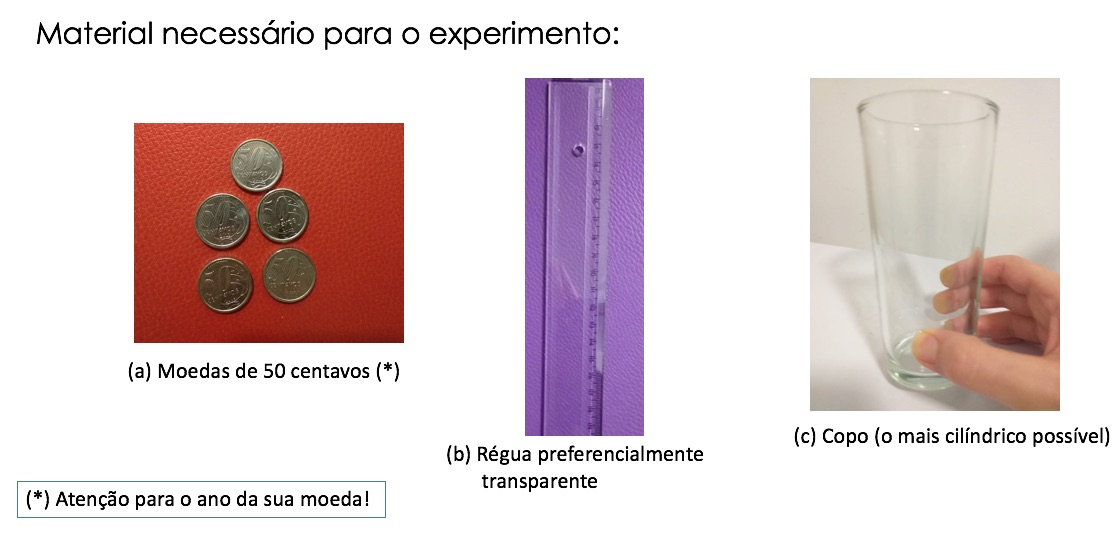
\includegraphics[height=0.28\paperheight]{Figuras_exp2/Foto1.jpg}
\caption{\label{fig:material} Material para o Experimento 2}
\end{figure}


\section{Procedimento experimental}
Antes de qualquer medida, se posicione de forma semelhante à sugerida na Figura~\ref{fig:observador}.

\begin{figure}[!hbt]
\centering
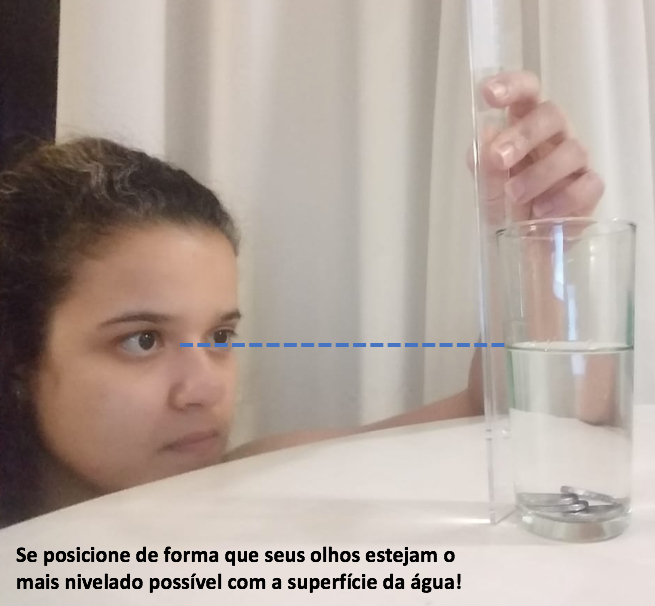
\includegraphics[height=0.28\paperheight]{Figuras_exp2/Foto2.jpg}
\caption{\label{fig:observador} Posicionamento do observador}
\end{figure}
\begin{enumerate}
\item {\bf A partir do volume de água deslocado}\\ 

Usando um copo cilíndrico parcialmente cheio d'água, introduza a(s) moeda(s) e estime o seu volume a partir do deslocamento do nível da coluna de água. No caso do copo, utilize uma régua para fazer essa medida a partir do registro dos níveis inicial e final.  Já com uma seringa descartável (Figura~\ref{fig:seringa}), o volume deslocado pode ser medido diretamente na seringa ao sugar a água, até que retorne ao mesmo nível da situação sem moeda(s), e lendo este volume na escala da própria seringa.  Dependendo do diâmetro do copo usado, avalie se o experimento deveria ser realizado com uma ou mais moedas de mesmo valor.

\begin{figure}[!hbt]
\centering
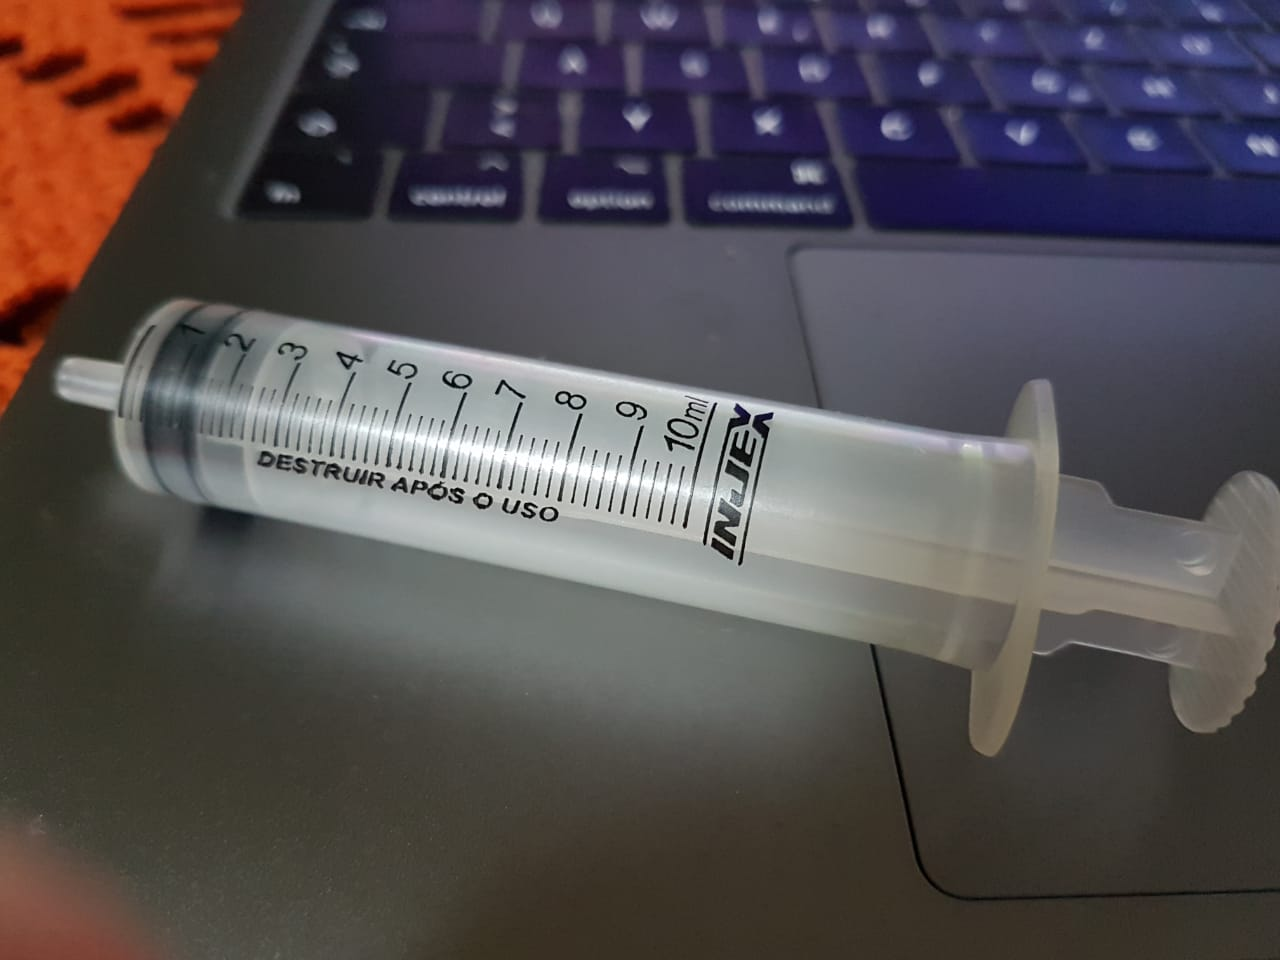
\includegraphics[height=0.18\paperheight]{Figuras_exp2/Foto3.jpeg}
\caption{\label{fig:seringa} Seringa}
\end{figure}


\item {\bf A partir da área da base da moeda  e de sua espessura}\\
Me\c ca  a espessura da moeda.  A área da base da moeda pode ser determinada  a partir da medição direta de seu diâmetro com uma régua ou a partir da medição de sua circunferência com o uso de um barbante e da régua.  Avalie qual procedimento é mais adequado.  A régua é o instrumento adequado para a determinação do 
di\^ametro da moeda? Nesse caso, tamb\'em avalie se o experimento deveria ser realizado com uma ou mais moedas do mesmo valor.

\item {\bf A partir da densidade volumétrica} \\
As moedas são fabricadas de forma padronizada  com relação às suas dimensões, massa e material.
Busque essas informações na Internet (página da Casa da Moeda). Fique atento que essas informações  podem variar de acordo com o ano de fabricação da moeda. A informação sobre o ano de fabricação consta na ``cara'' da mesma.
\end{enumerate}


\section{An\'alise de dados}
\begin{enumerate}
\item A partir dos valores  da espessura e do diâmetro ou circunferência da moeda,  medidos por você, calcule o volume da moeda utilizando uma das  fórmulas $V = \pi d^2 h/4  $ ($d =$ diâmetro e $h =$ espessura) ou $V=C^2 h/(4\pi)$ ($C =$ circunferência).

\item Sabendo que a densidade volumétrica do aço inoxid\'avel, dependendo da liga que o compõe, varia entre $7,8$ e $8,0$ g/cm$^3$, e utilizando o valor de massa padrão para a moeda utilizada, determine o seu volume e incerteza.
\item Organize em uma tabela os resultados obtidos para a determinação do volume da moeda com as respectivas incertezas para os três métodos realizados. Faça uma comparação entre os resultados obtidos. Leia  a segunda seção do Capítulo~\ref{sec:medidasDir&Indir} (Conceitos Básicos para Análise de Dados da Apostila). 
\end{enumerate}

\section{Discuss\~ao dos Resultados}
\begin{enumerate}
\item Qual foi a medição mais precisa? Justifique.
\item Considerando como referência o cálculo do volume da moeda a partir dos valores de suas dimensões encontrados na Internet, não os medidos por você, qual foi a medição mais exata? Justifique.
\item Justifique a vantagem de usar mais de uma moeda para o procedimento ``A partir do volume de água deslocado''.
\item   Os resultados encontrados são compatíveis entre si? Justifique. Esse resultado era esperado?
\item  Quais parâmetros contribuem mais fortemente para a incerteza do volume em cada um dos três métodos? Como essas incertezas poderiam ser diminuídas? Você sugere alguma modificação do procedimento experimental adotado?
\end{enumerate}



  %%% Nome original: Exp2_Roteiro_revisado.tex
%%%\input{PlanoInclinado_utf8}

\chapter{ Movimento de um corpo em queda vertical: determinação da aceleração da queda}
\label{chap:acelera}


\vspace{-0.7cm}

\section{Introdução}
Neste experimento determinaremos a aceleração de um corpo em queda vertical e vamos 
comparar o resultado obtido com o valor de referência da aceleração da gravidade ($g$)
para a cidade de Rio de Janeiro. 

Vamos analisar o movimento de queda vertical de um corpo cuja forma e tamanho apresente uma força de resistência do ar desprezível (por exemplo uma bolinha de gude) \footnote{Lembre que a queda vertical de um corpo quando a única força atuante sobre ele é a força da gravidade chama-se queda livre.}. Que tipo de movimento 
apresentaria o corpo se a força de resistência do ar fosse desprezível? \footnote{Lembre que o movimento da partícula é determinado através da Segunda Lei de Newton.}

Pense sobre o planejamento desse experimento. A aceleração do corpo pode ser obtida diretamente? Quais grandezas devem ser medidas para que seja possível obtê-la? Quais instrumentos são mais adequados para que esses dados possam ser coletados?

O experimento será discutido e guiado pelo roteiro abaixo. Siga o roteiro e as orientações do professor 
nos encontros remotos e vá fazendo suas anotações no caderno de laboratório. 

\section{Procedimento Experimental}

O arranjo experimental experimental está mostrado na Figura~\ref{fig:experimento}. Escolha uma bola de gude ou qualquer corpo arredondado de dimensões da ordem de grandeza da bolinha mostrada na Figura~\ref{fig:experimento}. Você deverá filmar a queda da bolinha com um celular, desde uma altura de, mais o menos, um metro. Para isso peça ajuda a uma pessoa que vai segurar a bolinha enquanto você filma.  Cole na parede uma régua de papel como está indicado na Figura~\ref{fig:experimento} \footnote {A régua não precisa ter a extensão de toda a trajetória a ser filmada, é somente uma referência de escala.}. Para a filmagem, posicione o celular num apoio com a tela do celular paralela à parede onde está colada a régua de papel. O celular deverá estar posicionado mais o menos no meio da trajetória da bolinha a uma distância da parede suficiente para poder filmar toda a queda de mais ou menos um metro. Não use ``slow-motion'' (câmera lenta),  filme com a velocidade normal do seu celular. A imensa maioria dos celulares filma a uma taxa de 30 frames/s \footnote{A palavra em inglês ``frame'' significa quadro.}. Verifique no seu celular se essa é a taxa usada.

Para analisar o filme da queda será usado o aplicativo Tracker para uso num computador 
que poderá ser baixado gratuitamente no link: 
\href{https://physlets.org/tracker/}{\textcolor {blue}
{https://physlets.org/tracker/}}
\footnote {O aplicativo é disponibilizado para os sistemas operacionais Windows, Linux e Mac OSX.}. 
O filme também poderá ser analisado com o aplicativo VidAnalysis disponível gratuitamente para celulares com sistema operacional Android no link  do
\href{https://play.google.com/store/apps/details?id=com.vidanalysis.free}{\textcolor {blue}
{Google Play}}. 
Os tutoriais de uso destes aplicativos estão disponíveis na forma de vídeos no site da \href{https://fisexp1.if.ufrj.br}{\textcolor {blue} {Física Experimental 1}} . 
No final do roteiro, encontram-se o Apêndice~\ref{sec:tracker} um tutorial básico do aplicativo Tracker, e um tutorial básico do aplicativo VidAnalysis no Apêndice~\ref{sec:vidanalysis}.  


\section{Análise de dados}
Usando o aplicativo Tracker ou alternativamente o aplicativo  VidAnalysis, monte a Tabela \ref{tabela1}.
\begin{table}[h]
\centering
\begin{tabular}{c|c|c|c|c}
t (s) & $y$ (cm) & $\delta y$ (cm)& $v_y$ (cm/s)& $\delta v_y$ (cm/s)\\
\hline 
&&&&  
\end{tabular}
\caption{Tabela de dados da experiência.}
\label{tabela1}
\end{table}
As colunas do tempo $t$ e da posição $y$ são preenchidas usando os aplicativos Tracker ou  VidAnalysis. As coordenadas $y$ correspondem às posições, por exemplo, do centro da bolinha ao longo da trajetória de queda, após ter escolhido o sistema de referência. Note que ao longo da trajetória a imagem da bolinha pode ficar um pouco embaçada como na Figura~\ref{fig:reguacomxis}.
Nesse caso, foi marcado com um ``x''  em azul 
o centro da bolinha enquanto que a barra vermelha é uma escolha razoável da região de incerteza
da posição do centro da bolinha.   A incerteza é uma fração do comprimento da mancha e depende da posição da bolinha.  

Para preencher a coluna da velocidade $v_y$ leia o Capítulo~\ref{sec:vinst} da Apostila.
Como são calculadas as incertezas $\delta v_y$?
\begin{itemize}
\item Em um papel milimetrado desenhe o gráfico $v_y \times t$ a partir dos dados da tabela indicando 
a incerteza nos valores das velocidades. Qual é a forma esperada para este gráfico?
\end{itemize}

  \begin{minipage}{\linewidth}
      \centering
      \begin{minipage}{0.25\linewidth}
          \begin{figure}[H]
              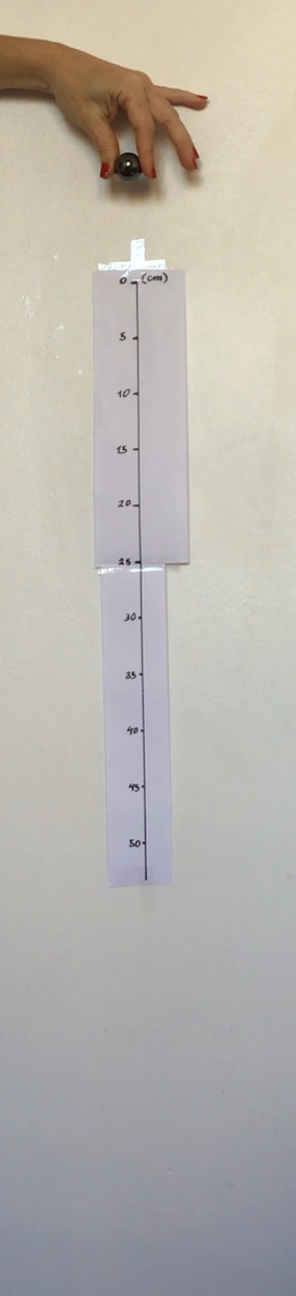
\includegraphics[width=\linewidth]{Figuras_exp3/fig1.pdf}
              \caption{\label{fig:experimento} Dispositivo experimental. Não esqueça de colar na parede uma régua de papel, como a indicada na Figura, para ser usada como referência na análise de dados.}
          \end{figure}
      \end{minipage}
      \hspace{0.05\linewidth}
      \begin{minipage}{0.3\linewidth}
          \begin{figure}[H]
              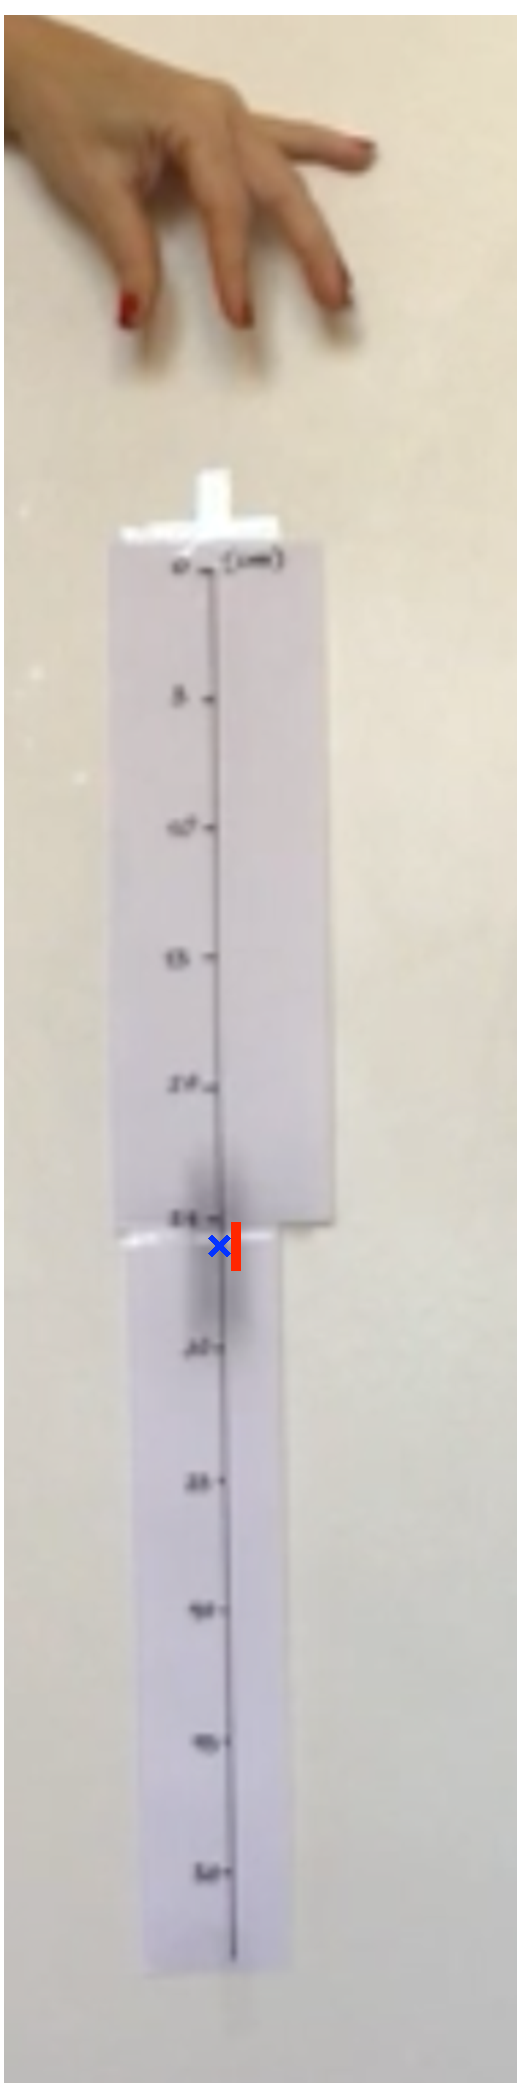
\includegraphics[width=\linewidth]{Figuras_exp3/fig2roteiro.pdf}
              \caption{\label{fig:reguacomxis}  Imagem da bolinha em plena queda. Note-se que a imagem, devido à alta velocidade, fica um pouco embaçada.}
          \end{figure}
      \end{minipage}
  \end{minipage}%

\begin{itemize}  
\item Use as colunas $t$, $v_y$ e $\delta v_y$ para  calcular através do Método dos Mínimos Quadrados (Seção~\ref{chap:minquad}  do Capítulo Conceitos Básicos para Análise de Dados da Apostila), qual é a melhor reta que aproxima os dados experimentais do gráfico $v_y \times t$?
\item Com os parâmetros da reta obtida no item anterior,  desenhe-a  na mesma folha de papel milimetrado 
onde fez o gráfico $v_y \times t$. Se você não conseguir achar um aplicativo que implemente o ajuste linear pelo método dos mínimos quadrados, desenhe a melhor reta que aproxima os dados experimentais 
pelo método visual (ver Seção~\ref{chap:minquad} do Capítulo Conceitos Básicos para Análise de Dados da Apostila) e obtenha os parâmetros que definem a reta 
(coeficiente angular $a$ e coeficiente linear $b$) escolhendo dois pontos na reta e substituindo na equação da reta $y=a\;t+b$.
\end{itemize}

\section{Discussão dos resultados}
\begin{enumerate}
\item A partir dos parâmetros do ajuste linear aos dados experimentais $v_y$ vs. $t$, 
como se obtêm o valor da aceleração de queda da bolinha?
\item 
Compare o valor da aceleração de queda da bolinha com o valor da aceleração da gravidade 
para a cidade do Rio de Janeiro que é $g=(978,7\pm 0,1)$ cm/$s^2$). 
Qual valor é mais preciso? Você utilizaria este método para determinar o valor da gravidade? Justifique.
\end{enumerate}


\section{Opcional: Estudo da conservação da energia}

%Também poderá entregar no arquivo pdf do relatório as seguintes tarefas opcionais:
\begin{enumerate}
\item Utilizando os dados registrados para a posição $y$ como função do tempo $t$, determine a altura $h$ da bolinha para cada instante de tempo, a partir do ponto mais baixo na Tabela~\ref{tabela1}.
\item Determine a energia cinética ($K$), energia potencial ($U$) e a energia mecânica ($E$) para cada intervalo de tempo. Para facilitar a organização das informações, construa uma tabela.
\item Faça um gráfico que contenha a energia cinética, potencial e mecânica em função do tempo.
\item Discuta a partir do gráfico obtido, se há ou não conservação da energia mecânica. Justificar.
\item No caso da energia não se conservar, determine o ganho ou perda percentual.
\end{enumerate}
\underline{\bf Observações:}
\begin{itemize}
\item Para os cálculos de energia considere a aceleração da gravidade no Rio de Janeiro, com 
sendo $g=(978,7 \pm 0,1)$ cm/$s^2$.
%\item Não esqueça de colocar todos os cálculos de propagação de incerteza num Apêndice.
\end{itemize}
\clearpage

\thispagestyle{plain} %%% Nome original: Exp3_Roteiro_revisado.tex

\chapter{Sistema de partículas -- Colisões}
\label{chap:colisao}
\vspace{-0.7cm}



\section{Introdução}
Neste experimento estudaremos colisões entre dois corpos. Em particular, procuraremos verificar experimentalmente se a conservação de momento linear total do sistema está presente. Também iremos ana-lisar uma possível conservação de energia mecânica total, explorando a diferença entre colisões elásticas e inelásticas. Na tomada de dados o movimento é gravado em um filme. A variação das posições dos corpos é analisada posteriormente. Programas de computador como aquele já utilizado no experimento anterior, o Tracker 
(Apêndice~\ref{sec:tracker}), são bastate úteis nessa análise. A análise do movimento com aplicativos no próprio celular é também possível.

A realização deste experimento em um curso remoto merece alguns comentários, dadas suas peculiaridades em relação à presença de atrito. Na versão presencial da disciplina de Física Experimental 1 da UFRJ, os alunos trabalham em sala com uma montagem usada para minimizar o atrito de dois carrinhos com a base: o trilho de ar. Em nosso curso remoto, os alunos não tem à disposição em casa uma ferramenta eficiente como o trilho de ar para minimizar o atrito. Assim, dividimos o experimento em duas partes. Na primeira parte o estudante faz a análise de dados experimentais nos moldes do curso presencial, porém utilizando dados obtidos previamente no Laboratório de Física Experimental 1. Na segunda parte (de realização opcional) o estudante faz a tomada de dados em casa, fazendo colidir objetos aos quais ele tem acesso fácil, como moedas. Este é um desafio final na disciplina: estudar colisões fora das condições controladas no laboratório didático, planejar e realizar sua montagem experimental, e analisar um sistema físico no qual as forças de atrito provavelmente serão observáveis. Para essa segunda parte, apontamos ainda uma versão simplificada do experimento que, fazendo suposiões sobre o atrito, permite fazer um teste da conservação de momento linear em uma colisão, mesmo sem o uso de celular ou computador \cite{Galante2020}. \footnote{{\it Two-penny physics: Teaching 2D linear momentum conservation}, Lorenzo Galante e Ivan Gnesi, American Journal of Physics {\bf88}, 279 (2020).} Outros exemplos de experimentos envolvendo colisões que os alunos podem fazer em casa estão na página da disciplina  \href{https://fisexp1.if.ufrj.br}{\textcolor {blue} {Física Experimental 1}} , no site do IF . 


\section{Colisão unidimensional sem atrito}

Neste experimento estudaremos as colisões e seu caráter elástico ou inelástico. Analisaremos as conservações de momento linear e energia mecânica de um sistema unidimensional de dois carrinhos que colidem entre si em um trilho de ar com atrito desprezível. Será utilizada uma gravação de um filme. Iremos analisá-la com o programa Tracker (Apêndice~\ref{sec:tracker}) para computador ou VidAnalysis (Apêndice~\ref{sec:vidanalysis}) para celular para levantamento de dados. O aluno também poderá usar outros programas ou aplicativos que permitam atingir os mesmos objetivos.

Pense sobre o planejamento desse experimento. Quais grandezas devem ser medidas diretamente para que seja possível avaliar as conservações de momento linear e energia mecânica? 

Siga o roteiro e as orientações do professor para fazer o experimento. Faça todas as anotações que julgar serem necessárias, elas serão importantes quando você for analisar os dados. Ao preparar o relatório,  tome como base as orientações do Apêndice ~\ref{sec:relatorios}  da Apostila do curso e as anotações realizadas durante o experimento. As discussões contidas no roteiro abaixo serão importantes para a elaboração do seu relatório.



Reflita sobre as seguintes questões e sugestões:

\begin{enumerate}
\item Qual é o objetivo desse experimento?
\item O que é um processo de colisão?
\item O filme mostra o movimento de dois carrinhos que deslizam sobre um trilho horizontal; há uma camada de ar entre o trilho e a base dos carrinhos, a fim de minimizar o atrito. Que tipo de movimento sobre o trilho é esperado para cada carrinho  antes e após a colisão? Pense nas forças que atuam sobre cada um deles.
\item  Considere a situação onde dois carrinhos colidem entre si ao se movimentarem sobre um trilho de ar horizontal com atrito desprezível; espera-se que tanto o momento linear como a energia mecânica se conservem nas colisões? O que define a diferença entre as colisões elástica e inelástica? Desenvolva as expressões matemáticas para conservação de momento linear e energia mecânica deste sistema unidimensional para os dois tipos de colisão, em termos das grandezas medidas no experimento. 
\item Como verificar experimentalmente se o momento linear do centro de massa do sistema é conservado?
\end{enumerate}

\vspace{-0.3cm}
\section{Procedimento Experimental e Levantamento de Dados}
Você terá acesso ao filme elasti.mp4 que deverá ser aberto com o programa Tracker ou VidAnalysis.
É interessante você observar esse filme: um carrinho (incidente), que chamaremos de $A$, move-se em direção a outro carrinho, denominado $B$, que está inicialmente em repouso. Ocorre o choque, mediado por ``para-choques''  feitos com elásticos esticados. Em seguida, $B$ passa a se mover, enquanto que $A$ continua a se mover, porém mais lentamente do que antes do choque. As massas dos carrinhos são $m_{A}=287,9 \pm 0,2$~g e $m_{B}=179,4 \pm 0,2$~g.
O comprimento total do trilho é $200$ cm; esse valor é importante para calibrar os comprimentos (escala da sua filmagem). Essa informação será usada quando for atribuir um valor à barra de medição do Tracker. Quando for estimar seu erro na calibração, note que há uma deformação da geometria do trilho no filme.

\begin{enumerate}
\item Proceda fazendo a tomada de dados da posição dos dois carrinhos antes e depois do choque. Precisaremos, para cada carrinho, aproximadamente 10 pontos antes e 10 pontos depois do choque. Entretanto, para minimizar o erro nas velocidades determinadas, é aconselhável que esses pontos não sejam “instantes sucessivos" registrados pelo Tracker ou VidAnalysis. 
Você pode escolher um intervalo de $0,1$ s no seu registro de dados (há vários ``frames''  do Tracker
ou VidAnalysis entre eles). 
\item  Analise o movimento de cada carrinho (tomada de dados) separadamente. Você terá que escolher um ponto de referência em cada carrinho para acompanhá-lo “manualmente" no programa.
Então terá que estimar a incerteza da sua medida de posição: amplie a imagem
e estime com que precisão consegue identificar o ponto de referência. Por exemplo, para uma ampliação de $200$ vezes, a incerteza é da ordem de $3$ mm.
\item Lembre-se de escolher um único sistema de referência para a determinação da posição em função do tempo. 
\item Construa uma tabela da posição de cada carrinho em função do tempo. 
\end{enumerate}

\section{Análise de dados e discussão dos resultados}
\begin{enumerate}

\item O instante de colisão pode ser obtido diretamente a partir da tabela dos dados?  Faça um gráfico da posição em função do tempo para os dois carrinhos e determine o instante em que eles colidem. 
\item Determine as velocidades dos carrinhos antes e depois da colisão a partir do ajuste linear dos dados. Alternativamente, você pode usar o método gráfico para tal determinação. As duas abordagens estão descritas em apêndices na apostila do curso.
\item Analise o comportamento do momento linear e da energia mecânica do sistema antes e depois do choque. Houve conservação dessas grandezas? Que conclusões você pode tirar desses resultados?
%\item Faça uma previsão dos valores das velocidades finais que você espera em função do modelo teórico.
%\item Compare os valores para as velocidades finais obtidas experimentalmente com as previstas no ponto anterior.  Discuta.

\item Calcule a porcentagem de perda de energia cinética, dada por:
\[
\frac{| K_f - K_i|}{K_i}
\]
\noindent
onde $K_i$ e $K_f$ são a energia cinética inicial e final, respectivamente. Discuta os resultados obtidos.
\end{enumerate}


%\item Calcule a posição do centro de massa em função do tempo (adicione as colunas correspondentes na tabela de posição dos carrinhos em função do tempo) e adicione estes pontos ao gráfico de posição em função do tempo já realizado. O momento linear se conserva?
%\item O resultado obtido para a conservação (ou não) do momento linear observando-se o deslocamento do centro de massa do sistema está de acordo com o obtido analisando-se o movimento dos dois carrinhos separadamente?  
%\item Determine a velocidade do centro de massa antes e depois da colisão a partir do ajuste linear. Discuta.

%{\bf Observação:} Lembre de colocar todos os cálculos de propagação de incertezas num Apêndice, anexado ao Relatório, claramente explicados.
\chapter{Colisões (Opcional)}
\label{chap:colisaoopcional}
\vspace{-0.7cm}
%\let\clearpage\relax
\thispagestyle{empty}
\section{Introdução}

Neste experimento propomos um estudo de colisões entre dois corpos, que o aluno pode executar todo em casa. O sistema físico estudado é composto por duas moedas apoiadas sobre uma superfície lisa. Uma delas está inicialmente em repouso e a outra é lançada sobre ela, deslizando. Nosso foco é explorar quais grandezas se alteram e quais se conservam durante a colisão. Analisamos o momento linear e a energia mecânica das moedas individualmente e, muito importante, do sistema formado pelas duas juntas.

Agora em duas dimensões, a pergunta básica feita antes no seu experimento unidimensional sobre o momento linear total do sistema se divide em duas: Há conservação do momento linear total na direção $x$? Há conservação do momento linear total na direção $y$? A energia é uma grandeza escalar e continuamos perguntando: A energia mecânica total E do sistema se conserva na colisão estudada? 

Uma diferença fundamental entre este e o estudo que utilizou a filmagem do trilho de ar é a presença aqui de uma força atrito sobre cada moeda enquanto ela se desloca. Propomos explorar uma diferença qualitativa entre (i) as forças de atrito entre as moedas e a superfície e (ii) as forças de contato entre as moedas. As forças de contato, ditas {\it forças impulsivas}, são muito mais intensas que as forças de atrito, mas atuam apenas durante a colisão em si. O efeito das forças de atrito sobre as moedas no curto intervalo de tempo durante o qual elas interagem é muito pequeno: durante a colisão dominam as forças de contato. Assim, a discussão sobre conservação de momento e energia durante a colisão continua basicamente a mesma da situação sem atrito.

Este roteiro usa como exemplo o choque entre duas moedas de 1 Real, e indica dois caminhos para a análise da colisão. Use o exemplo fornecido para se ambientar com o estudo de colisões, mas não se preocupe em reproduzir as trajetórias mostradas ou em usar também moedas de 1 Real. Lance uma de suas moedas em direção à outra, e analise o resultado da colisão entre as duas. As sugestões para registrar o movimento e analisar os dados estão nas próximas seções. Na primeira sugestão para análise, a informação sobre a colisão vem de medidas da distância percorrida depois da colisão por cada uma das moedas \cite{Galante2020} e do ângulo entre essas duas trajetórias.  Na segunda, são feitas medidas diretas de posição em função do tempo com uma taxa alta o suficiente para revelar o caráter impulsivo das forças de contato~\cite{deJesus2016}
%\cite{deJesus2016}.

Neste experimento você tem liberdade na organização de um relatório a ser encaminhado ao professor. Note que é importante que seu texto tenha suporte em uma ou mais imagens relativas à sua montagem experimental e às análises gráfica e/ou numérica do movimento.


%o movimento depois da colisão até as duas moedas atingirem o repouso, depois de dissipar toda sua energia cinética em decorrência das forças de atrito.\cite{Galante2020}. Na segunda, fazemos medidas diretas de posição em função do tempo 

%a informação é obtida a partir dos traços defi  
%analise o movimento até as duas moedas atingirem o repouso depois de dissipar toda sua energia cinética em decorrência das forças de atrito.

%Sugerimos duas estratégias para a análise de conservação de momento linear. Na primeira se restrinja a poucos quadros antes e depois da colisão. Na segunda, analise o movimento até as duas moedas atingirem o repouso depois de dissipar toda sua energia cinética em decorrência das forças de atrito.

%Por fim, seguem algumas observações sobre sua empreitada. Capriche na sua montagem experimental, mas não seja tão perfeccionista que acabe não fazendo o experimento do início ao fim. Também não se preocupe se você não consegue entender o que está por trás de cada detalhe do movimento. Você pode aprender bastante tentando modelar o sistema físico estudado em sua casa à partir do que está aprendendo em suas aulas teóricas. Mas repare como é também importante  descrever suas observações e as condições nas quais elas são feitas, e ressaltar pontos interessantes entre seus resultados.

%Na tomada de dados o movimento é gravado em um filme. A variação das posições dos corpos é analisada posteriormente. Programas de computador como aquele já utilizado no experimento anterior, o Tracker, são bastate úteis nessa análise.

%Para essa segunda parte, apontamos ainda uma versão simplificada do experimento que, fazendo suposiões sobre o atrito, permite fazer um teste da conservação de momento linear em uma colisão, mesmo sem celular ou computador.

\section{Procedimento experimental}

\subsection{Realização das medidas}

O procedimento para realizar a colisão é simples: procure em sua casa uma superfície plana e lisa sobre a qual as moedas possam deslizar com o menor atrito possível. Dê um peteleco em uma das moedas, lançando-a em direção à outra. Teste diferentes superfícies. No caso mostrado como exemplo neste roteiro foi usada uma superfície de fórmica. Utilize um aparelho celular para filmar todo o experimento, desde o instante inicial do movimento até o repouso final das moedas.

Experimente diferentes velocidades iniciais do objeto incidente. Se a velocidade for muito baixa, o atrito fará a moeda incidente parar muito rápido, inviabilizando o experimento. Se a velocidade for alta demais, o celular não irá conseguir capturar imagens com uma taxa alta o suficiente para estudar o movimento. Fazer a filmagem no modo em câmera lenta pode ajudar. É comum que os celulares façam filmagens em seu modo padrão com taxa de 30 quadros por segundo (ou {\it frames per second} - fps). Possívelmente seu celular é capaz de fazer a filmagem em um modo em câmera lenta com 120 fps ou mais. Se esse for o caso, aproveite essa opção, mas certifique-se de que seu filme não seja comprimido antes da análise. Se usar 30 fps, faça o filme com muita luz, de preferência ao Sol, evitando assim imagens borradas.

Uma vantagem no uso das moedas é que suas massas podem ser descobertas com uma pesquisa na internet. O diâmetro das moedas também é informação de fácil obtenção {\it online}, e pode ser usada para calibrar as distâncias na análise dos dados. Use duas moedas iguais para que as forças de atrito sejam iguais.

\subsection{Análise das imagens}

\begin{figure}
\centering
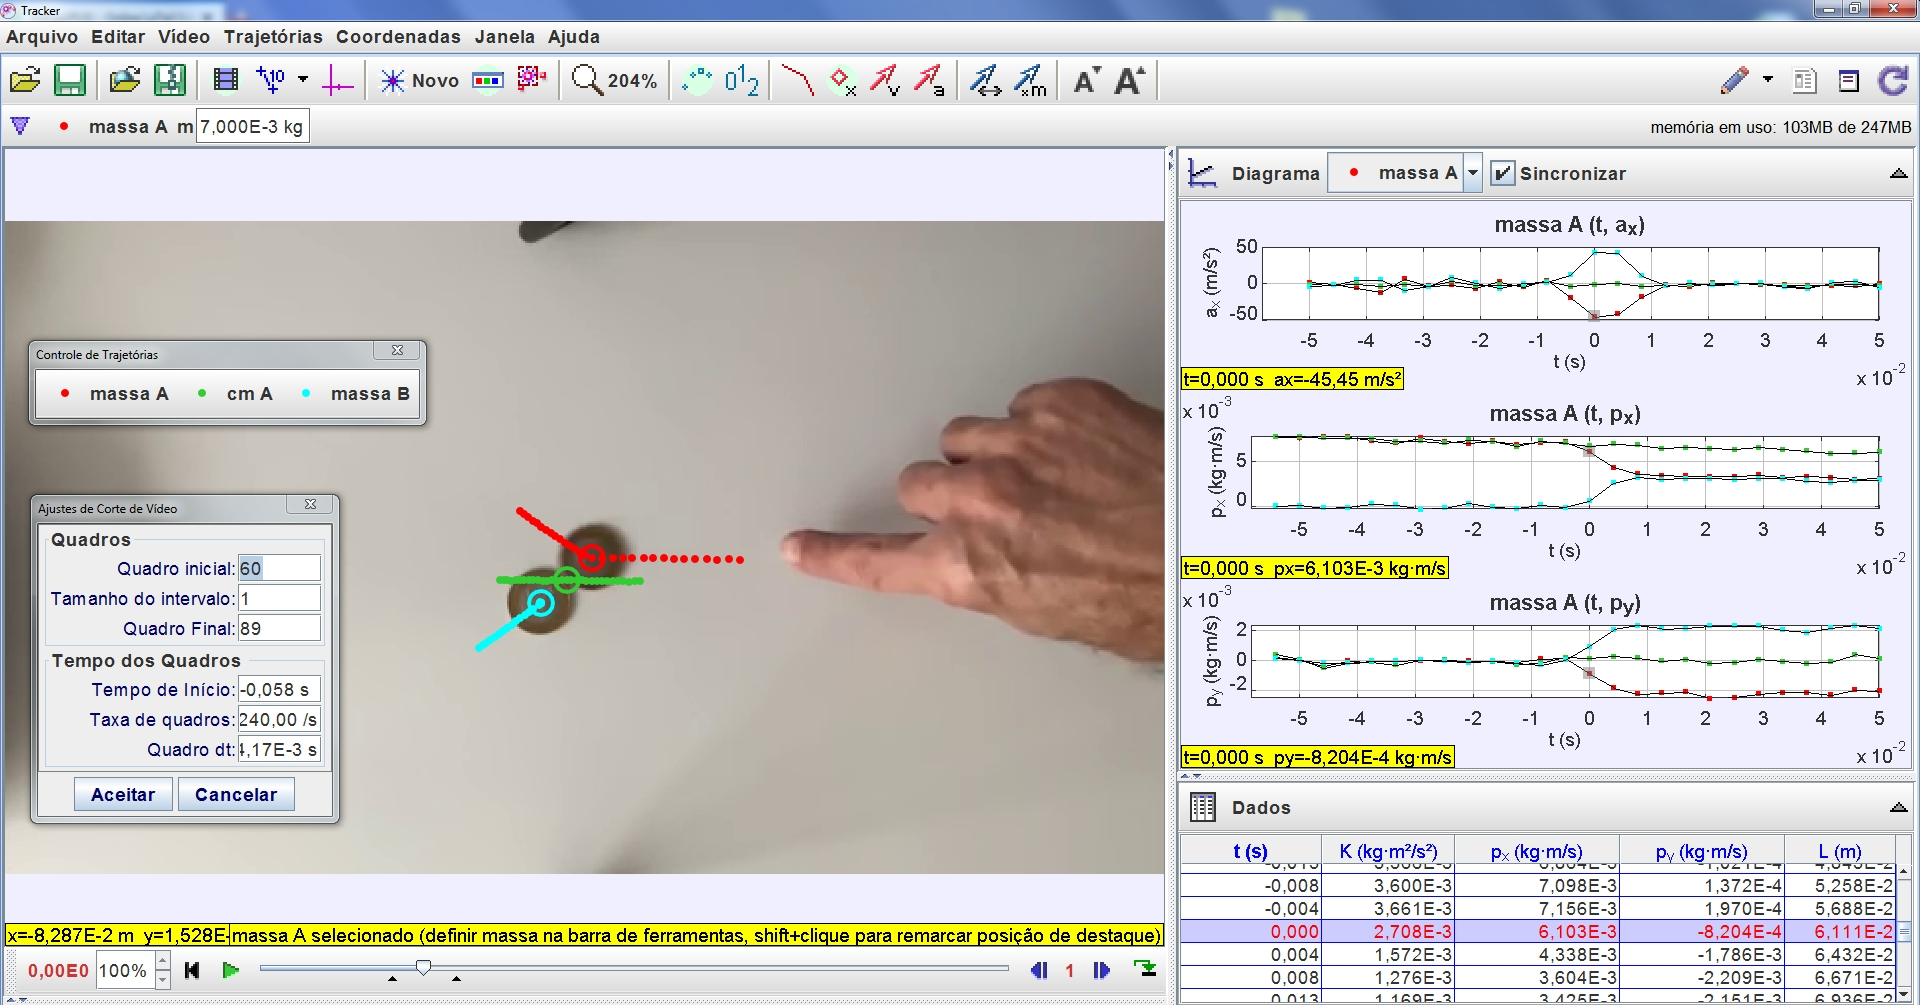
\includegraphics[width=0.7\columnwidth]{Figuras_exp4/figcolisaomoedas1.jpg}
\caption{\label{fig:figcolisaomoedas1} Tela típica de análise com o programa Tracker.}
\end{figure}

Os dois métodos sugeridos para análise da colisão baseiam-se em medidas de posição sobre imagens registradas em função do tempo. O programa Tracker (Apêndice~\ref{sec:tracker}), usado anteriormente no Experimento 3 e agora no 4, é uma ferramenta interessante para uso nos dois métodos. 

A partir de suas medições para as posições de cada um dos corpos, e de informação sobre suas massas, você poderá obter também a evolução da posição do centro de massa do sistema. Note que as forças de interação entre os dois objetos são internas ao sistema. Assim, não influenciam o movimento do centro de massa (CM), que deve ser mais simples que o movimento de cada um dos corpos. Analise o comportamento do CM do sistema antes, durante e depois da colisão.

Depois de importar seu filme para o Tracker, entre no programa com a informação sobre a taxa de quadros por segundo da sua filmagem. Dê um ``zoom'' nas suas imagens para marcar melhor as posições dos centros de massa de cada moeda. O próprio programa calcula e representa a posição do CM do sistema.

Com o programa Tracker você pode ainda gerar facilmente gráficos de velocidade, aceleração, momento linear, energia e outros. 
A Figura~\ref{fig:figcolisaomoedas1} mostra uma tela típica do Tracker em uma análise desse tipo, na qual os gráficos escolhidos são feitos automaticamente à medida que os pontos são marcados sobre a imagem. O programa utiliza para isso derivação numérica, mas você não precisa aqui se preocupar com os detalhes desse procedimento matemático. Se estiver curioso, pode ver na apostila um exemplo de derivação numérica na seção sobre  “Determinação da velocidade instantânea". Os gráficos de aceleração de cada um dos corpos são úteis para você entender o caráter impulsivo das forças de interação na colisão. Você pode também construir seus gráficos à mão ou utilizando um programa específico para essa função (consulte o Capítulo~\ref{chap:minquad} “representações gráficas"  da Apostila). 


%Sugerimos duas estratégias para a análise de conservação de momento linear. 

%Na primeira se restrinje a poucos quadros antes e depois da colisão. Na segunda, analise o movimento até as duas moedas atingirem o repouso depois de dissipar toda sua energia cinética em decorrência das forças de atrito.

 
\section{Exemplo de resultados e análise}


\subsection{ Medidas do traço de posição até o repouso das moedas}

\begin{figure*}
\centering
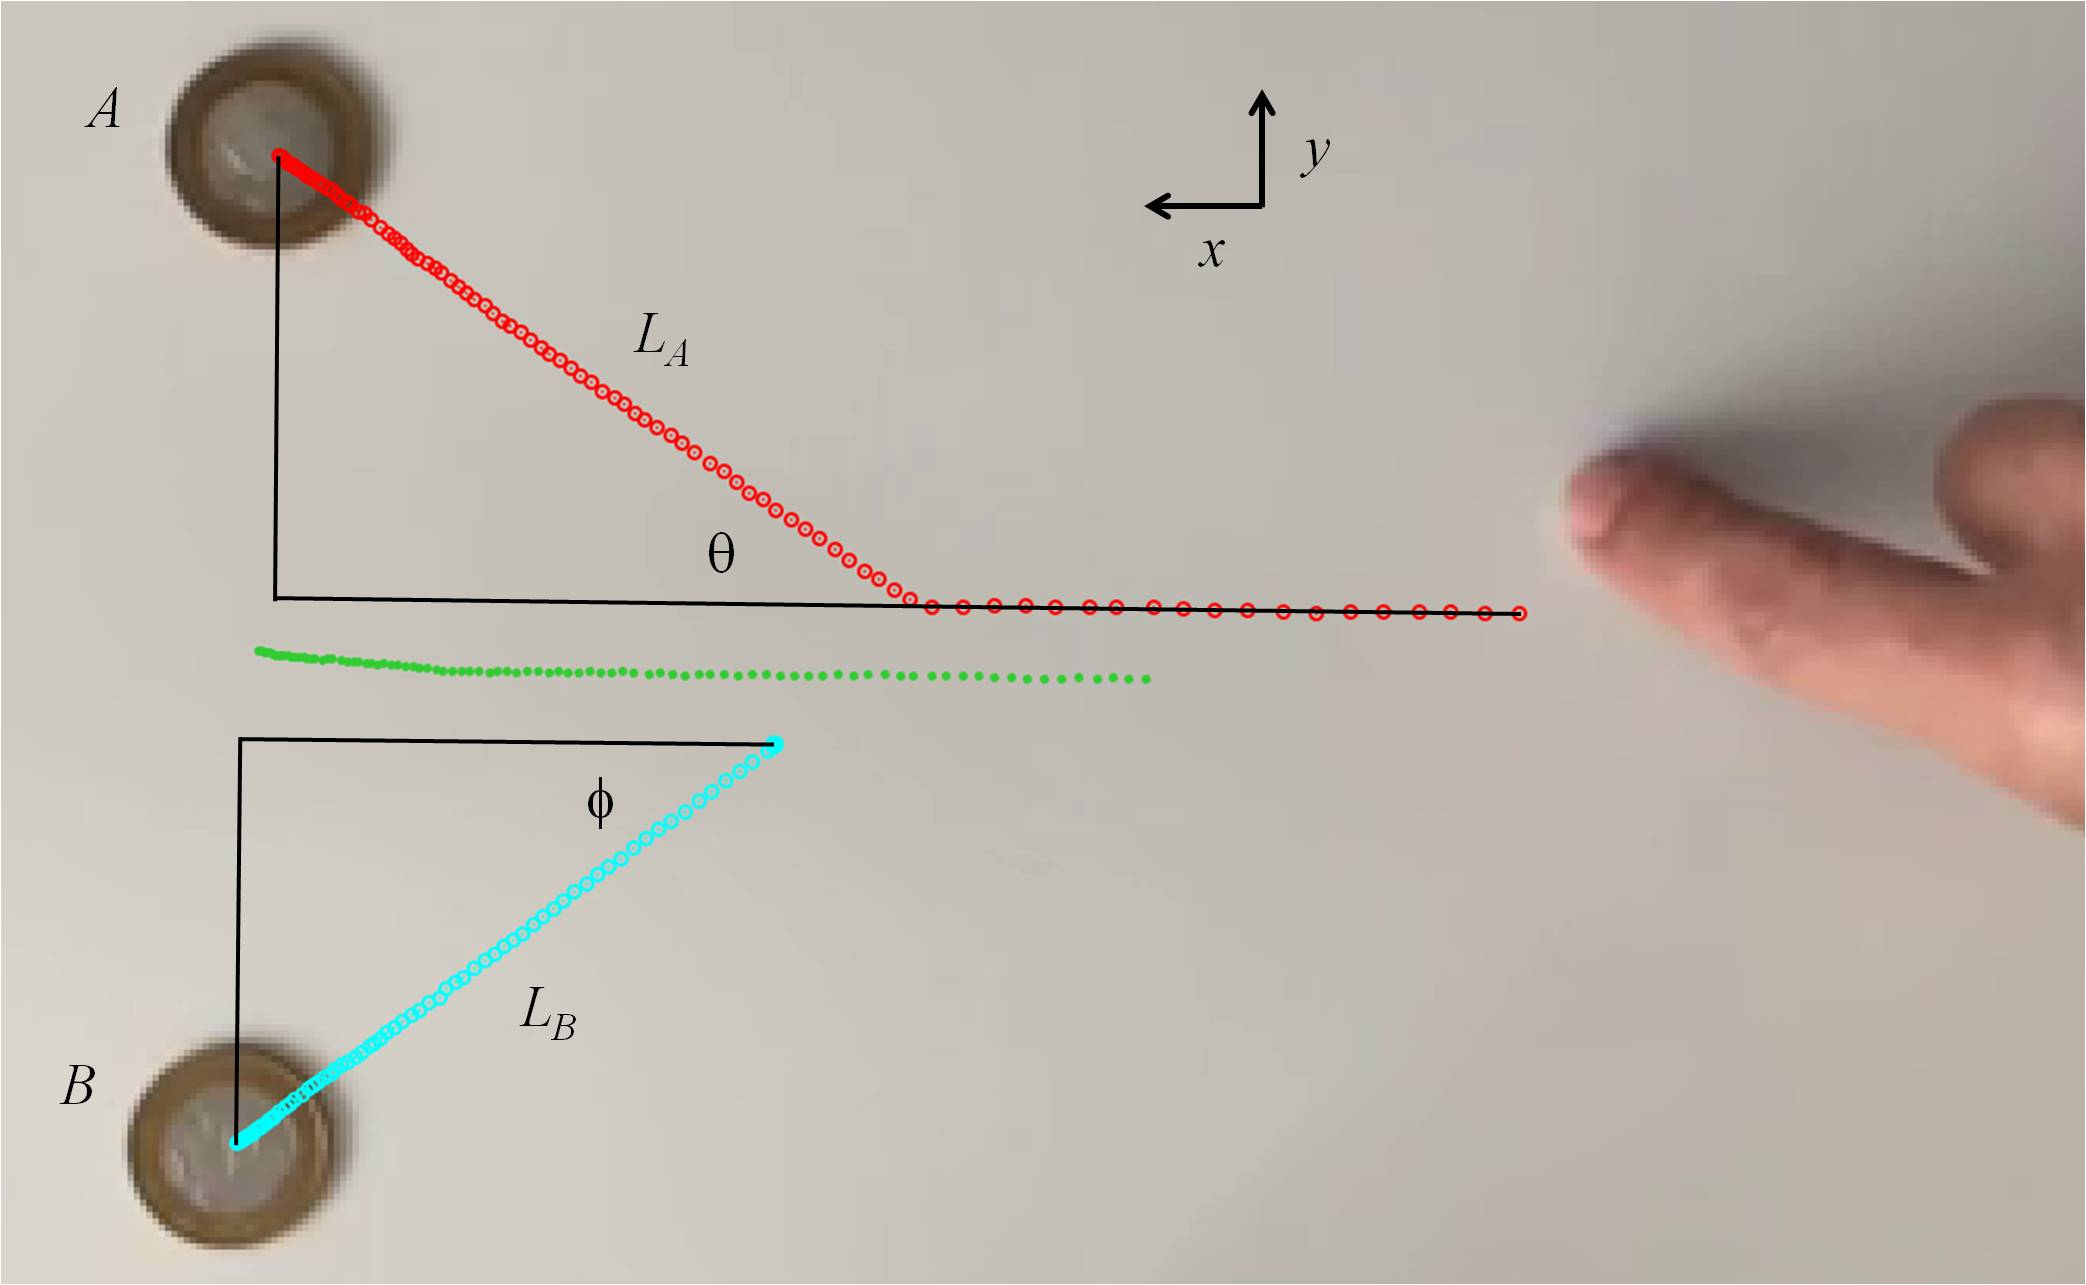
\includegraphics[width=0.5\columnwidth]{Figuras_exp4/figcolisaomoedas3.jpg}
\caption{\label{fig:figcolisaomoedas3} Moedas em suas posições finais e marcações de suas trajetórias (CM em verde).}
\end{figure*}

A primeira estratégia que indicamos para testar a conservação de momento linear na colisão de duas moedas, na presença de atrito, foi sugerida recentemente por Galante e Gnesi~\cite{Galante2020}.

Eles chamam a atenção para similaridades dela com métodos calorimétricos com os quais se mede o momento de uma partícula sub atômica a partir de um rastro que ela deixa em um detetor. Na versão simplificada com moedas colidindo, é assumido que a força de atrito é constante e o teorema trabalho-energia cinética é usado para estimar os módulos dos momentos lineares das duas moedas depois da colisão. Temos assim para cada moeda a relação entre o módulo de seu momento $p$ logo após a colisão e o alcance $L$ até parar:
\begin{equation}
\frac{p^2}{2m} = F_{at}~L, 
\end{equation}
onde $F_{at}$ é o módulo da força de atrito e $m$ é a massa da partícula. Se as moedas são iguais, $m$ e $F_{at}$ são iguais para as duas, e obtemos (ver Figura \ref{fig:figcolisaomoedas3}):
\begin{equation}
\frac{p_A}{p_B} = \sqrt{\frac{L_A}{L_B}}.
\end{equation}
Tomando a direção de incidência da moeda A em $x$, e considerando a moeda B inicialmente parada, a componente do momento linear total em $y$ antes da colisão é zero. Logo, devemos ter depois da colisão as componentes ${\text p}_{Ay}$ e ${\text p}_{By}$ com mesmo módulo e sinais contrários e, portanto, a razão entre elas deve ser igual a -1. Para testar essa hipótese, precisamos medir também os ângulos entre os momentos finais e a direção de incidência da moeda projétil, a fim de determinar 
\begin{equation}
\frac{{\text p}_{Ay}}{{\text p}_{By}} = -\frac{p_A~{\text sen}(\theta)}{p_B~{\text sen}(\phi)} = - \sqrt{\frac{L_A}{L_B}}~\frac{{\text sen}(\theta)}{{\text sen}(\phi)}.
\end{equation}

A partir da Figura \ref{fig:figcolisaomoedas3}, na qual foram marcadas as posições das moedas até elas pararem, obtemos 
$L_A=(0,111 \pm 0,003)$~m, 
${\text sen}(\theta)=(0,57 \pm 0,02)$, 
$L_B=(0,091 \pm 0,003)$~m, 
e ${\text sen}(\phi)=(0,60 \pm 0,02)$. 
Assim, obtemos experimentalmente, depois da colisão:
\begin{equation}
\frac{{\text p}_{Ay}} {{\text p}_{By}} = - 1,05 \pm 0,05.
\end{equation}
Este resultado mostra que a soma das componentes ${\text p}_{Ay}$ e ${\text p}_{By}$, dentro do erro experimental, permanece igual a zero depois da colisão. Verificamos assim que a componente $y$ do momento linear total se conservou nesse experimento.

A variação percentual de energia na colisão pode ser expressa como (dedução no Apêndice deste roteiro):
\begin{equation}
\frac{E_f - E_i}{E_i} = \frac{-1}{1+ \displaystyle {\frac{\sqrt{\frac{L_A}{L_B}}+\sqrt{\frac{L_B}{L_A}}}{2~ \cos(\theta+\phi)}}}.
\label{eqE}
\end{equation}
A Eq. \ref{eqE} mostra que se não houvesse perda de energia cinética na colisão, teríamos um ângulo entre os vetores momento final dos dois corpos $\theta+\phi=90^{\degree}$. No entanto,
da Figura \ref{fig:figcolisaomoedas3} temos $\theta+\phi= 72^{\degree}$ e $L_A/L_B=1,2$. Nesse caso, substituindo valores na Eq. \ref{eqE}, determinamos uma diminuição, devida à colisão, de $24\%$ na energia cinética total do sistema. A colisão é, portanto, inelástica. 

Note que você pode filmar a colisão, como feito aqui, mas isso não é essencial. No experimento original de Galante e Gnesi eles usam apenas moedas, lápis, papel, e régua. O preço da simplicidade neste método é assumir que a força de atrito é constante e igual, em módulo, para as duas moedas. 


\subsection{ Medidas de posição durante curto intervalo de tempo}

\begin{figure*}
\centering
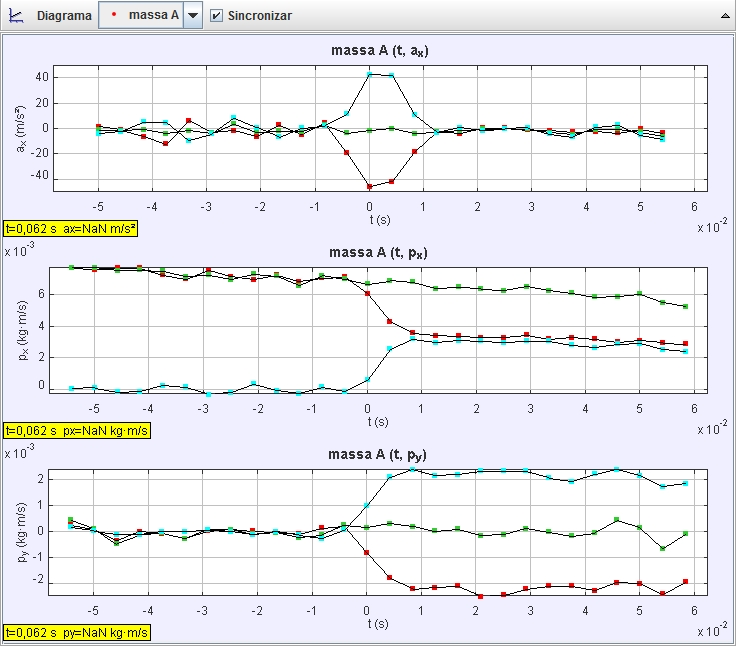
\includegraphics[width=0.7\columnwidth]{Figuras_exp4/figcolisaomoedas2.jpg}
\caption{\label{fig:figcolisaomoedas2} Gráficos de a$_x$, p$_x$ e p$_y$ em função do tempo. Moeda A em vermelho, moeda B em azul e  centro de massa do sistema moeda A mais moeda B em verde. }
\end{figure*}
Analisando apenas um curto intervalo de tempo antes e depois da colisão, o efeitos da força de atrito nas variações de momento linear em cada moeda serão pequenos em relação aos efeitos da força de contato entre as moedas. Os gráficos da Figura~\ref{fig:figcolisaomoedas1} estão reproduzidos com destaque na Figura~\ref{fig:figcolisaomoedas2}: aceleração na direção $x$ (direção dada pela moeda incidente), componente do momento linear na direção $x$, e componente do momento linear na direção $y$. Em cada gráfico é feita uma comparação dos valores associados à moeda A (em vermelho), à moeda B (em azul), e ao centro de massa do sistema moeda A mais moeda B (em verde). O gráfico da aceleração mostra no momento da colisão um pico para a moeda B e um pico invertido bastante similar para a moeda A. Esses picos refletem as forças de contato durante a colisão. Ainda no mesmo gráfico, vemos que a duração da colisão é de cerca de um centésimo de segundo. Para efeito de comparação, perceba que a aceleração de cada moeda chega, durante a colisão, a cerca de quatro vezes o valor da aceleração da gravidade, mas cai rapidamente quando apenas a força de atrito está presente. 

É possível demonstrar que o produto da massa pela área de cada um dos picos é igual à variação do momento linear. Assim, picos simétricos no gráfico de aceleração na Figura~\ref{fig:figcolisaomoedas2} demonstram a conservação do momento linear total do sistema, neste caso na direção $x$. Note que a aceleração do centro de massa é próxima de zero antes, durante e depois da colisão. A conservação de momento linear em $x$ e em $y$ durante a colisão pode ser vista também diretamente nos dois últimos gráficos da Figura~\ref{fig:figcolisaomoedas2}, ligeiramente mascarada por uma pequena e lenta variação do momento linear total devida às forças de atrito, que são externas ao sistema moeda A mais moeda B.


%Nesta segunda parte o aluno decide qual será sua montagem experimental feita em casa, filma a colisão com o celular, e faz a análise do movimento usando o programa Tracker, já utilizado anteriormante no curso.



%A seguir apresentamos uma sugestão de experimento a ser feito em casa: colisão bidimensional entre duas moedas no plano. Apresentamos imagens e um de conjunto de dados para você se familiarizar, mas lembre-se: o importante aqui é você obter e analisar seus prórios dados experimentais. Outras sugestões, como colisão entre bolinhas de gude e colisão entre blocos de gelo, estão em um arquivo separado na homepage da disciplina. Você pode escolher uma das três para fazer na sua casa ou ainda desenvolver uma ideia nova, sem perder de vista que nosso foco é o estudo do comportamento do momento linear total em colisões. 




%Por fim, seguem algumas observações sobre sua empreitada. Capriche na sua montagem experimental, mas não seja tão perfeccionista que acabe não fazendo o experimento do início ao fim. Também não se preocupe se você não consegue entender o que está por trás de cada detalhe do movimento. Você pode aprender bastante tentando modelar o sistema físico estudado em sua casa à partir do que está aprendendo em suas aulas teóricas. Mas repare como é também importante  descrever suas observações e as condições nas quais elas são feitas, e ressaltar pontos interessantes entre seus resultados.




%\thispagestyle{plain}
%%%\input{Rolamento_utf8}  %%% Não programado para o PLE 2020.1

\part[Conceitos Básicos para Análise de Dados]{Conceitos Básicos para Análise de Dados}
%%%%%\setcounter{chapter}{0}
\chapter{Medidas e incertezas}
\label{sec:medidasErro}
\vspace{-0.5cm}

Uma das maneiras para conhecer e descrever a natureza que nos rodeia é mediante a realização de observações experimentais, que chamamos de medidas. O primeiro problema com o qual nos encontramos é como os resultados encontrados podem ser comunicados de maneira clara, de forma que sejam compreensíveis e reprodutíveis por outros experimentadores. Para estabelecer o valor de uma grandeza (mensurando) temos que utilizar instrumentos e um método de medida, como também é necessário definir as unidades da medida. Por exemplo se desejamos medir a largura de uma mesa, o instrumento de medição será uma régua ou uma trena e, utilizando o sistema de unidades internacional (SI), a unidade que utilizaremos será o metro (m). A régua, portanto, estará calibrada nessa unidade ou em seus submúltiplos, como, por exemplo, centímetros e milímetros. O método de medição consistirá em determinar quantas vezes a unidade e as frações dela estão contidas no valor do mensurando.

Toda medição é afetada por uma incerteza que provém das limitações impostas pela precisão e exatidão dos instrumentos utilizados, da interação do método de medição com o mensurando, da definição do objeto a medir, e da influência do(s) observador(es) que realiza(m) a medição.

O que se procura em cada medição é conhecer o valor medido ($x$) e a sua incerteza ($\delta_x$) na de\-ter\-mi\-na\-ção do resultado, ou seja, determinar os limites probabilísticos destas incertezas.  Procura-se estabelecer um intervalo
\begin{equation}
x - \delta_x < x < x + \delta_x
\end{equation}
\noindent
como ilustrado na Figura~\ref{fig:Inter}, dentro do qual podemos dizer que o valor da grandeza se encontra, com uma certa probabilidade.  Em geral utiliza-se como incerteza um intervalo em torno do valor central com 68\% de probabilidade. 
\begin{figure}[h]
\begin{center}
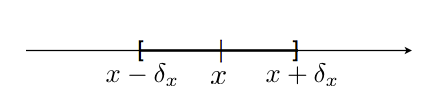
\includegraphics[width=10cm]{fig/IntervaloIncerteza}
\vspace{-0.5cm}
\caption{\label{fig:Inter} Intervalo de probabilidade para a grandeza medida, onde $x$ é o valor mais representativo da nossa medição e $\delta_x$ é a incerteza absoluta.}
\vspace{-0.5cm}
\end{center}
\end{figure}

Não existem regras para determinar o tamanho do intervalo, porque dependerá de muitos fatores do processo de medição. O tipo de medição, a figura da escala, a acuidade visual de quem esteja fazendo a medida, as condições de iluminação, etc, formarão parte na determinação da largura do intervalo de medição. A incerteza associada a uma medida deve ser determinada a cada vez que se faça a medição. Por exemplo, é comum pensar que quando fazemos uma medida com uma régua com escala graduada, a "incerteza de leitura (incerteza instrumental)" é automaticamente a metade da menor divisão. Um instrumento com divisões muito finas usado para medir um objeto com bordas mal definidas pode dar um intervalo de medição maior que várias das divisões menores. Contrariamente, um objeto bem definido com boas condições visuais pode permitir a identificação de um intervalo de medição muito menor que a menor divisão da escala. Cada situação deve ser avaliada de forma individual.
 
\vspace{-0.2 cm}
Uma forma usual de expressar o resultado de uma medição é:         
\begin{equation}
x \pm \delta_{x} 
\end{equation}
\noindent
e indicando a {\it unidade de medição}. Além disso é possível definir a {\it incerteza relativa} como:
\begin{equation}
\epsilon_x = \frac{\delta_x}{x} 
\end{equation}
\noindent
que expressa o quão significativa é a incerteza em relação a valor medido. Também pode-se calcular a {\it incerteza relativa percentual} como:
\begin{equation}
\epsilon_{\%} = \epsilon_x \cdot 100\% = \frac{\delta_x}{x} \cdot 100\% 
\end{equation}
\noindent

Por exemplo, ao medir o comprimento L de uma mesa podemos apresentá-lo como L=(1,00 $\pm$ 0,01) m ou L=1,00 $\pm$ 0,01 m, se encontramos um valor de 1,00 m, com uma incerteza de 1 cm em torno desse valor central encontrado. É importante apresentar sempre o valor central e a incerteza na mesma unidade. Essa medição tem um incerteza relativa de 0,01 (0,01/1,00) e uma incerteza relativa percentual de 1\%. A palavra {\bf precisão} muitas vezes é utilizada como sinônimo de incerteza relativa percentual. Note, no entanto, que nem sempre a precisão de uma medida corresponde à precisão do instrumento utilizado para realizá-la. A precisão de um instrumento será discutida em contraposição ao conceito de acurácia mais abaixo.
\newpage
\section*{Incertezas}
Os distintos tipos de incertezas podem ser classificados em:
\begin{itemize}
\item {\bf Incertezas do instrumento:} Os instrumentos de medição têm uma incerteza finita que está associada à variação mínima da magnitude que ele mesmo pode detectar. Por exemplo, se temos uma régua graduada em milímetros, não será possível detectar variações muito menores que uma fração de milímetro. Se, ao lermos o valor medido na régua, aproximamos para o valor inteiro em mm que mais se aproxima da medida, dizemos que a incerteza da régua é de 1 mm. Se, ao contrário, conseguimos identificar valores múltiplos de meio milímetro, então dizemos que a incerteza é de 0,5 mm. Não é, no entanto, razoável supor que conseguimos identificar a olho nú frações menores que 0,5 mm em uma régua milimetrada.

\item {\bf Incertezas estatísticas ou aleatórias:} São as devidas flutuações aleatórias na deter\-mi\-na\-ção do valor do mensurando entre uma medida e outra.  Estas flutuações ocorrem com igual probabilidade tanto para mais quanto para menos. Portanto, medindo várias vezes e calculando a média, é possível reduzir a incerteza significativamente. Estas incertezas são tratadas pela teoria estatística de erros de medição.

\item {\bf Incertezas sistemáticas:} Acontecem pelas imperfeições dos instrumentos e métodos de medição e sempre se produzem no mesmo sentido (não podem ser eliminados com várias medições). Alguns exemplos podem ser um relógio que atrasa ou adianta, uma régua que se dilata, o erro devido à paralaxe, etc... 
\end{itemize}

A interação do método de medição com o mensurando também pode introduzir erros.  Consideremos como exemplo a medição de temperatura para a qual utilizamos um ter\-mô\-me\-tro. Parte do calor do objeto que queremos medir flui ao termômetro (ou vice-versa), de maneira que o resultado da medição do valor da temperatura difere do original devido à presença do termômetro (interação que devemos realizar). Fica claro que esta interação pode ser desprezível, se, por exemplo, estamos medindo a temperatura de um litro de água, mas a quantidade de calor transferida ao termômetro pode ser significativa se a quantidade de volume é uma fração pequena de, por exemplo, um mililitro e utilizamos um termômetro convencional.

\section*{Precisão e exatidão}

A precisão de um instrumento ou um método de medida está relacionada à sensibilidade ou menor variação de uma grandeza que pode ser detectada com certo instrumento ou método. Dizemos que um paquímetro (por exemplo, com mínima divisão de 0,01 mm) é mais preciso que uma régua (mínima divisão 1 mm) ou que um cronômetro (por exemplo com mínima divisão 10 ms) é mais preciso que um relógio (mínima divisão 1 s), etc. Quanto menor a {\bf incerteza relativa} de uma medição, mais precisa ela é. É importante notar que o valor absoluto da incerteza isoladamente não  é suficiente para qualificar a precisão de uma medida. Por exemplo, reportar a distância entre Rio e São Paulo com incerteza de um metro certamente é muito bom. Por outro lado, medir o comprimento de um carro com incerteza de um metro é muito ruim. Qual a diferença? No primeiro caso, estamos falando de uma dúvida de um metro em cerca de 500 km e no segundo caso, a incerteza é de um metro em cerca de 4 metros.

Além da precisão, é importante realizar uma medição com exatidão ou, utilizando um termo mais antigo, acurácia. Esta está geralmente relacionada com a qualidade da calibração do instrumento utilizado ou o método de medição aplicado. Imaginemos que utilizamos um cronômetro para medir os tempos com uma precisão de 10 ms, mas sabemos que atrasa 1 minuto cada uma hora. Por outro lado, utilizamos um relógio com uma precisão de 1 s que marca a hora certa a todo instante. Neste caso vamos dizer que o cronômetro é o mais preciso, mas o relógio é o mais acurado. Um critério para se comparar a exatidão de duas medidas é dado pela menor discrepância relativa. A discrepância é definida como o módulo da diferença entre o valor medido e um valor de referência para a grandeza e a discrepância relativa é definida como o módulo da razão entre a discrepância e o valor de referência. Quanto menor a discrepância relativa de uma medida, mais exata ou acurada ela é.

Portanto, procuraremos sempre realizar uma medição utilizando um método que seja preciso e exato ao mesmo tempo.


\chapter{Medidas Diretas e Indiretas}
\label{sec:medidasDir&Indir}
\vspace{-0.5cm}
Para estabelecer o valor de uma grandeza temos que utilizar um instrumento de medi\c c\~ao e um m\'etodo de medi\c c\~ao. Al\'em disso, ser\'a necess\'ario definir as unidades em que essa magnitude \'e medida. Por exemplo, se queremos medir a largura de uma mesa, utilizaremos uma r\'egua e, dependendo do sistema de medi\c c\~ao escolhido, expressaremos o valor medido em unidades de comprimento como, por exemplo, o metro (m) para o sistema de unidades internacional (SI) ou centmetros (cm) no caso do CGS. O m \'etodo de medi\c c\~ao consistir\'a em determinar a quantidade de unidades da menor fra\c c\~ao da r\'egua que correspondem ao comprimento que se deseja medir. Quando uma medi\c c\~ao  \'e realizada lendo o resultado diretamente em um instrumento (constru\'ido para isso), dizemos que a {\bf medida \'e direta}. H\'a grandezas que n\~ao se medem diretamente, mas que s\~ao obtidas a partir de outras grandezas medidas de forma direta.  Por exemplo, para conhecer \'area de um ret\^angulo medem-se os comprimentos de seus lados ou para determinar o volume de uma esfera deve-se medir o di\^ametro.  Neste caso a {\bf medida \'e indireta}. 
% \'i
%\~ao
%\c c\~oes
\section*{Medidas diretas com flutua\c c\~oes aleat\'orias}\label{stat}

Consideremos uma grandeza da qual se fazem $N$ medi\c c\~oes diretas, que chamaremos: $x_1, x_2, x_3, ... , x_N$. Estes valores ser\~ao geralmente distintos entre si, mas alguns valores podem se repetir. 

Evidentemente n\~ao ser\'a satisfat\'orio fornecer como resultado da medi\c c\~ao uma tabela de $N$ valores. \'E necess\'ario caracterizar a s\'erie de medi\c c\~oes mediante uns poucos par\^ametros que tenham um significado preciso relacionado com a magnitude medida e/ou o processo de medi\c c\~ao utilizado. Os par\^ametros importantes s\~ao:

\begin{enumerate}
\item {\bf Valor m\'edio} \'e  a m\'edia aritm\'etica dos valores medidos
\begin{equation}
\bar{x} = \frac{1}{N} \sum_{i = 1}^N {x_i},
\label{eq:vm}
\end{equation}
\noindent
e é o valor atribu\'ido \`a magnitude medida. É bastante intuitivo considerar a m\'edia aritm\'etica como valor representativo da grandeza medida. A m\'edia aritm\'etica se caracteriza por apresentar as medições ao seu redor, de modo que a soma dos desvios 
\begin{equation}
\delta_i = x_i - \bar{x} ,
\end{equation}
\noindent
é igual a zero. Ou seja,
\begin{equation}
S = \sum_{i=1}^N \delta_i = 0.
\end{equation}

Isto pode ser facilmente demonstrado, escrevendo:
\begin{equation}
S = \sum_{i=1}^N \delta_i =  \sum_{i=1}^N (x_i - \bar{x}),
\end{equation}
\noindent
e distribuindo o somatório, de modo que:
\begin{equation}
S = \sum_{i=1}^N x_i - \sum_{i=1}^N \bar{x}  =  \sum_{i=1}^N x_i - N\bar{x}.
\end{equation}

Utilizando a expressão do valor médio (equação~\ref{eq:vm}):
\begin{equation}
\sum_{i=1}^N x_i = N\bar{x},
\end{equation}
\noindent
obtemos $S = 0$ como queríamos mostrar.

Por esta razão, a soma dos desvios não é um parâmetro que possa ser utilizado para caracterizar a distribuição das medições ao redor do valor médio e é necessário utilizar outro parâmetro.

\item Dispersão das medições ou {\bf desvio padrão} define-se como:
\begin{equation}
\sigma = \sqrt{\frac{\sum_{i=1}^N (x_i - \bar{x})^2}{N-1}}.
\end{equation}
\noindent

O desvio padrão é um parâmetro que caracteriza o processo de medida. Quando as medições são poucas, $\sigma$ pode flutuar, mas para muitas medidas ($N$ grande) estabiliza-se e não depende do número de medições.

\item O {\bf erro ou incerteza do valor médio} é definido como:

\begin{equation}
\xi=\sqrt{\sigma_{m}^2 + \sigma_{r}^2},
\end{equation}

\noindent
onde $\sigma_{m}$ está associado às flutuacões estatísticas em torno do valor médio:

\begin{equation}
\sigma_{m}=\frac{\sigma}{\sqrt{N}},
\end{equation}

\noindent
e $\sigma_{r}$ expressa os erros sistemáticos residuais (por exemplo devido à um instrumento mal calibrado).

Vamos supor que nas nossas medidas não ocorrem tais erros sistemáticos, de forma que usaremos sempre:

\begin{equation}
\xi=\frac{\sigma}{\sqrt{N}},
\end{equation}


O erro do valor médio é a dispersão esperada para as médias de várias séries de medições realizadas nas mesmas condições. O erro do valor médio depende do número de medições como se pode ver na sua expressão, sendo que ela diminui com o aumento do número de medições.



\end{enumerate}

\section*{Medidas Indiretas}\label{prop}

Como j\'a foi definido anteriormente, h\'a grandezas que não podem ser determinadas diretamente, mas que se obt\'em a partir de outras grandezas que, estas sim, são medidas de forma direta. Portanto, as incertezas das grandezas que se medem diretamente devem ser propagadas para contribuir à incerteza da grandeza que se calcula utilizando uma determinada expressão.

Sejam $x_1, x_2, ... , x_N$ grandezas independentes medidas de forma direta, e seja a grandeza que se quer determinar $F = F (x_1, x_2, ..., x_N)$ uma função das grandezas $x_1, x_2, ... , x_N$, cujas incertezas estão dadas por $\delta{x_1}, \delta{x_2}, ... , \delta{x_N}$. Pode-se mostrar que a incerteza de $F$ é dada por: 
\begin{equation}
(\delta F)^2 = \left(\frac{\partial F}{\partial x_1}\right)^2 \cdot \delta{x_1}^2  +  \left(\frac{\partial F}{\partial x_2}\right)^2 \cdot \delta{x_2}^2 + ... +  \left(\frac{\partial F}{\partial x_N}\right)^2 \cdot \delta{x_N}^2,  
\end{equation}
\noindent
ou
\begin{equation}\label{eq:propag-geral}
(\delta F)^2 = \sum_{i = 1}^N \left(\frac{\partial F}{\partial x_i}\right)^2 \cdot \delta{x_i}^2 .
\end{equation}
Esta equação é a f\'ormula de propagação da incerteza para uma grandeza determinada indiretamente.%, ler capítulo 8 do livro de Vuolo para ver a demonstração de esta fórmula.

\section*{Compara\c c\~ao entre duas medidas da mesma grandeza}
Muitas vezes comparamos diferentes resultados experimentais para a medida de uma mesma grandeza.  Estes resultados podem vir por exemplo das diferentes técnicas utilizadas para determinar uma grandeza, ou podem vir de valores conhecidos tabulados na literatura. Vamos supor que temos dois resultados para uma mesma grandeza sendo o primeiro $x_1 \pm \delta{x_1}$ e o segundo $x_2 \pm \delta{x_2}$.  Se eles são estimativas de uma mesma grandeza, esperamos que a discrepância entre eles ($|x_1-x_2|$) seja compatível com zero. Como cada uma das medidas está sujeita a uma flutuação estatística de acordo com sua incerteza, em geral encontramos valores diferentes de zero para a discrepância. Como podemos avaliar se a discrepância é significativamente diferente de zero ?  Há várias formas de se fazer essa avaliação, dependendo do grau de confiança que queremos ter na afirmação de que a diferença é incompatível com zero (ou equivalentemente de que os dois valores são incompatíveis entre si) . Vamos considerar a discrepância entre os valores ($|x_1-x_2|$) pouco significativa ou irrelevante quando for menor que 3 vezes a incerteza da discrepância. Utilizando a expressão para propagação de incertezas definida na Seção~\ref{prop}, determinamos a incerteza da discrepância $\delta |x_1-x_2|=\sqrt{\delta x^2_1+\delta x^2_2}$. Resumindo, duas medidas independentes $x_1$ e $x_2$ da mesma grandeza são consideradas {\bf  compatíveis} quando : 
$$|x_1 - x_2| < 3 \sqrt{\delta x^2_1+\delta x^2_2}$$ 
ou
$$\frac{|x_1 - x_2|}{\sqrt{\delta x^2_1+\delta x^2_2}}<3.$$

Ao contrário, consideramos as duas medidas $x_1$ e $x_2$ {\bf incompatíveis} quando a discrepância entre elas é maior que 3 vezes a incerteza da discrepância. 

 Considere por exemplo a medida de um comprimento de uma mesa cujo resultado é L$_{exp}$=(98~$\pm$~1)~cm. Como podemos ver se esse resultado é compatível com o valor nominal fornecido pelo fabricante, que é de L$_{nom}$=1 m ? 
Como o valor nominal nesse caso não tem incerteza, a incerteza  da discrepância é igual à incerteza da medida experimental. A discrepância é de 2 cm, que é apenas duas vezes a incerteza da discrepância e a medida é, portanto, compatível com o valor nominal. Uma outra forma de ver isso \'e analisando se o valor nominal est\'a contido no intervalo de valores $I_{exp}$=[L-3$\delta L$, L+3$\delta$L]. Nesse caso, o valor 100 cm est\'a contido no intervalo $I_{exp}$=[95,101] cm.

Em um outro exemplo, um estudante mede o valor da aceleração da gravidade e encontra $g_{exp}=9,21\,\pm\,0,01$ m/s$^2$ e quer comparar com o valor tabelado $g=9,787\,\pm\,0,001$ m/s$^2$. Temos:
$$\frac{|g_{exp} -g |}{\sqrt{\delta g^2_{exp}+\delta g^2}}=\frac{0,577}{0,01005}\approx 57\gg 3.$$
Logo, os dois valores são incompat\'iveis.



\section*{Exercícios}

\begin{num}

\item Os lados de um paralelepípedo são $a$ = (4,50 $\pm$ 0,05) cm, $b$ = (8,50 $\pm$ 0,09)~cm e $c$ = (35,0 $\pm$ 0,3) mm. Determinar o volume do cubo com sua incerteza absoluta e relativa.

\item Na medição da resistência (R), se obteve o valor da tensão V = (15,2 $\pm$ 0,2)~V e da corrente I = (2,6 $\pm$ 0,1)~A. Qual é a incerteza absoluta da resistência usando a equação R = V/I?
 
\item Um pêndulo simples é utilizado para medir o valor da aceleração da gravidade utilizando equação:

\[ 
T = 2 \pi \sqrt{\frac{l}{g}}.
\]
\noindent
O período $T$ medido foi de (1,24 $\pm$ 0,02)~s e o comprimento do pêndulo $l$ = (0,381 $\pm$ 0,002)~m. Qual é o resultado do valor da aceleração da gravidade $g$ com sua incerteza absoluta e relativa?

\item Para medir o comprimento total de um pêndulo (fio + esfera) usou-se uma régua milimetrada para medir o comprimento do fio e um paquímetro para medir o diâmetro da esfera. Observam-se os seguintes valores com as suas respectivas incertezas: 
\begin{iten}
\item[ ]Comprimento do fio = 2,100 m			
\item[ ] Incerteza comprimento do fio = 0,5 cm
\item[ ]Diâmetro da esfera = 2,114 cm			
\item[ ] Incerteza do diâmetro da esfera = 0,01 mm
\end{iten}
\noindent 
Ache o comprimento total e a sua incerteza associada.

\item Para o cálculo do volume de uma esfera, foi dado o raio da mesma: R = (232,0 $\pm$ 0,1)~mm. Calcular seu volume com a sua respectiva incerteza relativa.

\item A partir da figura~\ref{fig:fig1}, com as seguintes medidas:
\begin{iten}
\item[ ] L1 = (5,00 $\pm$ 0,05) cm
\item[ ] L2 = (20,00 $\pm$ 0,05) mm
\item[ ] L3 = (15,00 $\pm$ 0,01) mm
\end{iten}
\begin{figure}[t]
\begin{center}
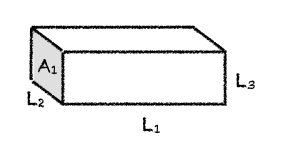
\includegraphics[width=8cm]{fig/Fig1}
\caption{\label{fig:fig1} Bloco retangular.}
\vspace{-0.4cm}
\end{center}
\end{figure}
\begin{num}
\item Determine a área A1 com a incerteza correspondente.
\item Determine o volume desta peça com a incerteza correspondente.
\item Se a precisão necessária para o resultado da área é de 0,5\% podemos considerar este resultado satisfatório?
\end{num}

\item Para determinar a altura de uma cachoeira, algumas pessoas mediram o tempo de queda de pedrinhas que eram soltas, em queda livre, de um mesmo local. Conhecendo o tempo de queda $t$, pode-se calcular a altura $h$ a partir da relação cinemática $h = 1/2 g t^2$ em que $g$ é a aceleração da gravidade. Foi utilizado um cronômetro com precisão de centésimos de segundo e os valores $t_i$ obtidos em 8 medidas estão na seguinte tabela:

\begin{center}
  \begin{tabular}{|>{ \centering\arraybackslash}m{1cm}  |>{ \centering\arraybackslash}m{2cm} |}  \hline
    	& t(s)	 \\ \hline	 	
  1	& 1,30\\ \hline	 
2	&1,09\\ \hline	 
3	&1,03\\ \hline	 
4	&1,27\\ \hline	 
5	&1,18\\ \hline	 
6	&1,31\\ \hline	 
7	&1,24\\ \hline	 
8	&1,15\\ \hline	 
  \end{tabular}
  \end{center}

Considerando $g = (9,784 \pm 0,001)$~m/s$^2$, calcule a altura da cachoeira e a sua incerteza.

\end{num}


\chapter{Algarismos Significativos}
\label{algSig}
\vspace{-0.5cm}
Imagine que você pergunta a hora a uma pessoa com um relógio de pulso analógico, como o mostrado na Figura~\ref{fig:relogio}. Essa pessoa dá uma olhada no relógio,  e responde: são 10 horas e 42 minutos. Voc\^e entende que o ponteiro dos minutos certamente estava entre o 8 e o 9, ou seja, corresponde a um valor entre 40 e 45 minutos, mais pr\'oximo de 40 do que de 45. Dizemos que esse algarismo que foi estimado, o 2,  \'e um {\bf algarismo duvidoso}. Os outros algarismos são {\bf algarismos certos}: o ponteiro das horas estava entre 10 e 11, com certeza. O conjunto de algarismos certos e duvidosos são os {\bf algarismos significativos da medida}. Quanto maior for o número de algarismos significativos em uma medida, mais informação ela traz. 

\vspace{-0.5cm}
\begin{figure}[hp!]
\begin{center}
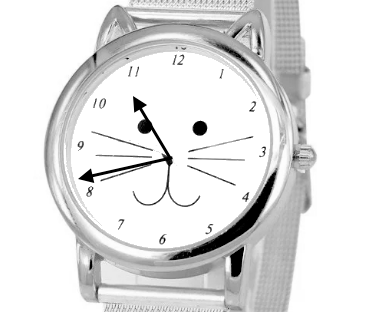
\includegraphics[width=5cm]{fig/relogioHoraPB}
\caption{Relógio marcando hora.}
\label{fig:relogio}
\end{center}
\end{figure}
\vspace{-0.5cm}
Quando realizamos uma medi\c c\~ao direta de uma grandeza, a partir da leitura de um instrumento anal\'ogico, que apresenta uma escala, o procedimento que se usa para fazer o registro do valor da grandeza \'e anotar todos os algarismos fornecidos pela escala do instrumento, eventualmente acrescentando mais um algarismo, que represente uma fra\c c\~ao da menor divis\~ao da escala do instrumento. No exemplo acima, do rel\'ogio, ao estimar 42 minutos, a pessoa imaginou uma escala de subdivis\~ao da menor divis\~ao do rel\'ogio em 5 partes, cada uma delas correspondendo a 1 minuto, e estimou que o ponteiro estava mais perto de duas subdivis\~oes. Quando o instrumento \'e digital, o m\'ultiplo da menor medida que ele pode fazer corresponde ao algarismo duvidoso do valor lido. Em um cron\^ometro digital com resolu\c c\~ao de 1 cent\'esimo de segundo, que mede um intervalo de tempo de 12,04 s, o 4 \'e o algarismo duvidoso da medida direta.

Um ponto que sempre gera dúvida é se os zeros são significativos ou não. Para responder, pense em alterar as unidades da medida. Se o número de zeros mudar ao fazer essa alteração, eles não são significativos, já que indicam apenas em que unidades estamos escrevendo a medida.  A medida ${x_1}=2,\!47$ cm tem três algarismos significativos, sendo o 7 duvidoso. Para escrever ${x_1}$ em metros, caminhamos a vírgula para a esquerda duas casas decimais e completamos com zeros. Nada foi feito em termos de alterar a quantidade de  informação em ${x_1}$, apenas trocamos as unidades, logo esses zeros de preenchimento não são significativos. Em resumo, as duas formas abaixo são equivalentes e têm três algarismos significativos:
\[
x_1=\underbrace{2,\!47}_{\mbox{\tiny sig}}\mbox{ cm} = 0,\!0\underbrace{247}_{\mbox{\tiny sig}}\mbox{ m}
\]
%
A mudança para uma unidade menor pode ser feita com ajuda de potências de dez, que não contam como algarismos significativos. Por exemplo, a medida ${x_2}$, com dois algarismos significativos pode ser escrita nas formas equivalentes
\[
{x_2}= 0,\!\underbrace{52}_{\mbox{\tiny sig}}\mbox{ kg} = 0,\underbrace{\!52}_{\mbox{\tiny sig}} \times 10^{3}\mbox{ g}  = \underbrace{5,\! 2}_{\mbox{\tiny sig}} \times 10^{2}\mbox{ g}
\]
%
Se escrevermos uma medida como ${x_3}=3,\!10$ s, ficará implícito que temos certeza dos três segundos e do um décimo de segundo. O zero na casa dos centésimos de segundo é duvidoso, sendo o último algarismo significativo da medida. Os zeros ao final do número são significativos. Observe mais um exemplo:
\[
\underbrace{100}_{\mbox{\tiny sig}}\mbox{ m}= 0,\underbrace{\!100}_{\mbox{\tiny sig}}\mbox{ km} = \underbrace{1,\!00}_{\mbox{\tiny sig}}\times 10^{8}\;\mu\mbox{m}
\]
%
Também aqui os dois algarismos zero à direita do 1 são significativos, independentemente da unidade que escolhamos para registrar o valor. Ao todo o comprimento registrado tem 3 algarismos significativos.

\section*{Incertezas e algarismos significativos}
%
%
Normalmente usamos um ou dois algarismos significativos para representar as incertezas, dependendo do grau de estimativa envolvido na sua determina\c c\~ao. Como vamos trabalhar com muitas estimativas na determina\c c\~ao das incertezas nas medidas diretas, usaremos a conven\c c\~ao de um significativo. Assim, o valor da medida deve ser escrito at\'e a casa decimal afetada pela incerteza, como nos exemplos abaixo.
%
\[
L = (2,\!25\pm 0,\!05)\mbox{ cm} \;\;\;\;\;\;\;\;  M = (351 \pm 2)\times 10^{-2}\mbox{ kg}
\]

No caso da incerteza de medidas indiretas, em geral \'e preciso arredondar o valor determinado a partir da propaga\c c\~ao das incertezas das medidas diretas, explicado no Capítulo~\ref{sec:medidasDir&Indir}.

Para arredondar um determinado valor,  vamos adotar os critérios da norma técnica da Associa\c c\~ao Brasileira de Normas T\'ecnicas ABNT-5891:
%
\begin{enumerate}
%
\item quando o algarismo a ser conservado for seguido de um algarismo inferior a 5, permanece inalterado o algarismo a ser conservado e retiram-se os posteriores (1,6357 arredondado à primeira casa decimal torna-se 1,6);
%
\item quando o algarismo a ser conservado for seguido de um algarismo superior a 5, ou igual a 5 seguido de no mínimo um algarismo diferente de zero, soma-se uma unidade ao algarismo a ser conservado e retiram-se os posteriores (1,6678 torna-se 1,7 e 1,6505 torna-se 1,7, arredondados à primeira casa decimal);
%
\item Se o algarismo à seguida do algarismo a ser conservado for igual a 5 e não houver mais nenhum algarismo à sua direita ou se todos os algarismos à direita forem zeros, retira-se todos os algarismos posteriores ao que será conservado e :
\begin{enumerate}
\item adiciona-se uma unidade ao algarismo conservado, se este for ímpar;
\item permanece inalterado o algarismo conservado, se este for par.
\end{enumerate}
%
\end{enumerate}
%
Observe os arredondamentos abaixo, feitos de modo a que a medida tenha 3 algarismos significativos e seguindo os critérios acima:
\begin{itemize}
%
\item $x = 4,678$ m $\rightarrow x = 4,\!68$ m 
\item $y = 4,674$ m $\rightarrow x = 4,\!67$ m 
\item $z = 4,675$ m $\rightarrow x = 4,\!68$ m  
\item $w = 4,665$ m $\rightarrow x = 4,\!66$ m 
%
\end{itemize}

Como exemplo, vamos calcular o peso $p$ da massa $m=(234,\!40\pm 0,02)$g sabendo que $g=(9,\!7879\pm 0,\!0001)$ m/s$^2$. 
Vamos trabalhar no SI, portanto escrevemos $m=(234,\!40\pm 0,\!02)\times 10^{-3}$ kg. Com isso,
%
\[
 p =  m \;   g = 2,\!29428376 \mbox{ N}
\]
%
Agora vamos calcular a incerteza. Como temos um produto,
\[
\left(\frac{\delta_p}{  p}\right)^2=\left(\frac{\delta_m}{  m}\right)^2+\left(\frac{\delta_g}{  g}\right)^2=\left(\frac{0,\!02}{234,\!00}\right)^2+\left(\frac{0,\!0001}{9,\!7879}\right)^2=7,\!409\times 10^{-10}
\]
Logo, 
\[
\delta_p=2,\!29428376 \mbox{ N}\times 2,\!72 \times 10^{-5}=6,\!23\times 10^{-5} \mbox{ N}
\]
Agora escrevemos a incerteza calculada com um significativo: 
\[
\delta_p = 6\times 10^{-5} \mbox{ N}
\]
Finalmente escrevemos $  p$ até a quinta casa decimal, usando o critério de arredondamento, e escrevemos o resultado final:
\[
2,\!2942\underline{8}376 \mbox{ N}\rightarrow p = (2,\!29428\pm 0,\!00006)\mbox{ N}
\]
%
Claro que também poderíamos usar a equação (\ref{eq:propag-geral}) para calcular a incerteza absoluta:
\[
\delta_p =  \sqrt{ (  m\delta_g)^2+(  g \delta_m)^2}.
\]
%
%\newpage
%


%

%\begin{comment}
%
%
%
\section*{Regra de bolso sobre algarismos significativos}
%
Muitas vezes o cálculo da incerteza propagada pode ser bem longo e fica difícil de saber se o resultado está certo ou não. Uma forma simples de saber se pelo menos a ordem de grandeza da incerteza propagada está correta é usar a seguinte regra:
%
\begin{itemize}
%
\item Numa operação matemática envolvendo medidas com diferentes números de algarismos significativos o resultado terá aproximadamente o mesmo número de algarismos significativos que a medida com menor número.
%
\end{itemize}
%
%

Vamos calcular o volume $V$ de um tubo de seção reta quadrada de lado $a=(2,\!0\pm0,\!1)$ cm e comprimento $L=(120,\!0\pm 0,\!1)$ cm.  
A medida $a$ tem 2 algarismos significativos e $L$, 4, sendo a mais precisa. Assim esperamos que $V$ tenha entre 2 e 4 algarismos significativos. Vamos fazer a propagação:
\[
V=a^2L\;\;\rightarrow\;\;   V =   a^2  L= 120,\!0\mbox{ cm}^3 
\]
%
\[
\left(\frac{\delta_V}{  V}\right)=\sqrt{\left(2\frac{\delta_a}{  a}\right)^2+\left(\frac{\delta_L}{  L}\right)^2}=0,\!1000034722
\]
Um erro muito comum é esquecer que 0,1000034722 é a incerteza  relativa e escrever este valor como se fosse a incerteza absoluta.

Calculando corretamente a incerteza absoluta, temos
\[
\delta_V=  V\left(\frac{\delta_V}{  V}\right)= (480,\!0\mbox{ cm}^3)( 0,\!1000034722) = 48,001666656 \approx 4,8001666656 \times 10  \mbox{ cm}^3
\]
Finalmente,
\[
V = (48\pm 5) \times 10 \mbox{ cm}^3\;
\]
O resultado final tem dois algarismos significativos, como a medida menos precisa usada no cálculo. Se for necessário melhorar a precisão da medida de $V$, vale a pena medir $a$ com mais precisão. Note que ao escrevermos o resultado final, utilizamos a mesma potência de 10 para $V$ e para sua incerteza $\delta_V$. Assim podemos saber qual deve ser o último algarismo a ser conservado no valor da medida e realizar o arredondamento, se necessário. Neste caso, o arredondamento foi feito na casa da unidade de $1\times 10 \mbox{ cm}^3$.
%

%\end{comment}
\section*{Exercícios}

%\vspace{-0.7cm}

Expresse corretamente os resultados para as seguintes medições com suas respectivas incertezas.
\begin{center}
\vspace{-1cm}
  \begin{tabular}{|c | c | c | c |>{ \centering\arraybackslash}m{8cm} |}  \hline
    & Medição	& Incerteza	& Unidades	& Resultado \\ \hline	 	
    1 & 67,002 & 0,023 & cm & \\ \hline
2 & 0,001 & 2,3 & erg & \\ \hline
3 & 45612,98 & 345 & cm/s & \\ \hline
4 & 14 & 29 & erg & \\ \hline
5 & 152,389 & 0,037 & cm/s$^2$ & \\ \hline
6 & 74,58 & 3,14 & g & \\ \hline
7 & 0,0012 & 0,0001 & m & \\ \hline
8 & 120034 & 2607 & m/s$^2$ & \\ \hline
9 & 45,98 & 2,1 & erg & \\ \hline
10 & 65555,467 & 56,001 & g & \\ \hline
11 & 23,456 & 1,2 & m & \\ \hline
12 & 0,173 & 0,056 & cm$^3$ & \\ \hline
13 & 45001,6 & 657,31 & J & \\ \hline
14 & 45,629 & 2,5914 & km/h & \\ \hline
15 & 104104 & 104 & m$^2$ & \\ \hline
16 & 0,0826 & 0,099 & cm/s & \\ \hline
17 & 3,69 & 1,582 & mm$^3$ & \\ \hline
18 & 19,78 & 5,46 & kg & \\ \hline
19 & 0,458 & 0,177 & cm & \\ \hline
20 & 135,589 & 0,0888 & g & \\ \hline
21 & 25,36 & 0,84 & cm & \\ \hline
22 & 74589,589 & 5698,26 & erg & \\ \hline
23 & 0,145 & 0,5 & cm/s & \\ \hline
24 & 14580,8 & 37,36 & erg & \\ \hline
25 & 125,369 & 0,041 & cm/s$^2$ & \\ \hline
26 & 74,58 & 3,14 & g & \\ \hline
27 & 0,025 & 0,0074 & m & \\ \hline
28 & 256 & 0,5 & m/s$^2$ & \\ \hline
29 & 7489 & 2,1 & m/s$^2$ & \\ \hline
30 & 4789,4 & 36,001 & g & \\ \hline   
  \end{tabular}
\end{center}


\begin{center}
  \begin{tabular}{|c | c | c | c |>{ \centering\arraybackslash}m{8cm} |}  \hline
    & Medição	& Incerteza	& Unidades	& Resultado \\ \hline	 
18 & 19,78 & 5,46 & kg & \\ \hline
19 & 0,458 & 0,177 & cm & \\ \hline
20 & 135,589 & 0,0888 & g & \\ \hline
21 & 25,36 & 0,84 & cm & \\ \hline
22 & 74589,589 & 5698,26 & erg & \\ \hline
23 & 0,145 & 0,5 & cm/s & \\ \hline
24 & 14580,8 & 37,36 & erg & \\ \hline
25 & 125,369 & 0,041 & cm/s$^2$ & \\ \hline
26 & 74,58 & 3,14 & g & \\ \hline
27 & 0,025 & 0,0074 & m & \\ \hline
28 & 256 & 0,5 & m/s$^2$ & \\ \hline
29 & 7489 & 2,1 & m/s$^2$ & \\ \hline
30 & 4789,4 & 36,001 & g & \\ \hline
  \end{tabular}
\end{center}

\chapter{Representações gráficas}
\label{sec:graf}
\section{Como fazer um histograma}
\label{sec:histo}

Quando fazemos uma análise estatística de um conjunto de $N$ medidas de uma determinada grandeza, podemos realizar um gráfico no qual se representa para cada valor (ou intervalo de valores) o número de vezes em que este aparece. Este tipo de gráfico recebe o nome de {\bf Histograma}. Um exemplo é mostrado na Figura~\ref{fig:histo}. Como o conjunto de valores obtidos é discreto, resulta um esquema de barras. A largura destas barras é a menor diferença entre os valores medidos ou o tamanho do intervalo escolhido no caso em que seja conveniente agrupar vários valores num intervalo (isto deve ser determinado em função da série de medições realizadas). O número de barras depende do conjunto de dados e do número total de medições. 

\begin{figure}[h]
\begin{center}
\vspace{-1.5cm}
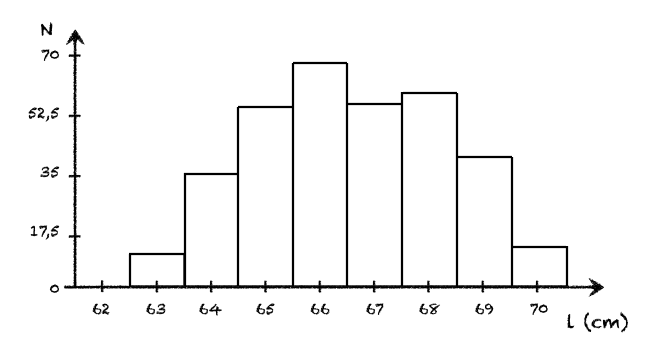
\includegraphics[width=12cm]{fig/HistogramWhite}
\vspace{-0.7cm}
\caption{\label{fig:histo} Exemplo de um histograma.}
\vspace{-1.cm}
\end{center}
\end{figure}
%-___ fim

Para que fique mais claro, vamos considerar o seguinte exemplo.  Medimos a altura de uma garrafa de água 40 vezes obtendo os seguintes valores, em centímetros:

\begin{center}
\hspace{-0.8cm}
  \begin{tabular}[m]{c c c c c c c c}
 20,3	 & 20,1 & 20,2 & 20,5 & 20,2 & 19,7 & 20,6 & 20,4\\
 19,8 & 20,3 & 20,1 & 20,2 & 20,3 & 20,4 & 20,3 & 19,6\\
 20,0 & 19,5 & 20,7 & 20,3 & 20,1 & 20,7 & 20,5 & 20,5\\
 20,5 & 20,3 & 20,4 & 20,2 & 20,3 & 20,2 & 20,6 & 20,8\\
 20,4 & 20,0 & 19,9 & 20,6 & 20,8 & 19,7 & 20,9 & 20,3\\
  \end{tabular}
\end{center}
\vspace{-0.3cm}

Como podemos ver, há valores que se repetem e a frequência de repetição é diferente para cada valor. Esta informação pode ser apresentada em forma gráfica, mediante a construção de um histograma. Para isto devemos escolher valores ou intervalos de valores e determinar quantas vezes o valor se repete no conjunto de dados.

Para nosso exemplo, vamos escolher intervalos de 0,2 cm começando pelo menor valor medido de 19,5 cm.  Desta forma o primeiro intervalo será de 19,5 a 19,7 cm, o segundo de 19,7 cm a 19,9 cm e assim sucessivamente.  Cada intervalo será representado no gráfico pelo seu valor central, ou seja, para o primeiro será 19,6 cm, para o segundo 19,8 cm, etc.  Como os intervalos são contínuos devemos escolher como serão os limites dos intervalos, aberto e fechado, pois, por exemplo, o valor 19,7 cm vai contar para o primeiro ou o segundo intervalo. No nosso exemplo, o valor inferior vai ser o fechado e o valor superior o aberto (ou seja, 19,7 cm vai contar para o segundo intervalo e não para o primeiro). Desta forma, podemos construir a Tabela~\ref{tab:freq}, de frequências:
\begin{table}[!htbp]
\begin{center}
\hspace{-0.8cm}
\caption{Tabela de frequências absolutas e relativas em função da altura medida de uma garrafa.}\label{tab:freq}
  \begin{tabular}[m]{|c| c| c| c|}
  Intervalo (cm) & Valor do Intervalo (cm)	& Frequência & Frequência Relativa (\%)  \\
19,5 - 19,7	&	19,6	&	2   & 5,0 \\
19,7 - 19,9	&	19,8	&	3   & 7,5\\
19,9 - 20,1 	&	20,0	&	3   & 7,5\\
20,1	- 20,3	&	20,2	&	7   & 17,5\\
20,3 - 20,5	&	20,4	&	12 & 30,0\\
20,5 - 20,7	&	20,6	&	8   & 20,0\\
20,7 - 20,9	&	20,8	&	4   & 10,0 \\
20,9	- 21,1	&	21,0	&	1   &  2,5\\ 	
  \end{tabular}
\end{center}
\end{table}
\vspace{0.3cm}

Uma vez construída a tabela, podemos fazer o gráfico no qual vamos colocar no eixo-x os valores centrais dos intervalos escolhidos e no eixo-y o número de repetições (Frequência). Para isto deve ser escolhida uma escala adequada em cada eixo, de forma que a distância entre todos os valores centrais dos intervalos seja constante.  Para o caso do eixo-y, a escala deve ser escolhida de forma tal que o valor mais repetido fique na parte superior do eixo, de forma que possa ser apreciada a estrutura do histograma. Uma vez escolhida a escala, uma barra será desenhada para cada intervalo com o tamanho da frequência determinada na tabela anterior, como mostramos no lado esquerdo da Figura~\ref{fig:histoexemplo}.

Uma forma alternativa de se fazer o histograma é colocando no eixo-y a frequência relativa, ou seja, o número de repetições dividido pelo número total de medidas, frequentemente mostrado em percentagem, como na última coluna da Tabela~\ref{tab:freq} e no histograma do lado direito da Figura~\ref{fig:histoexemplo}. 

\begin{figure}[h]
\begin{center}
\begin{tabular}{cc}
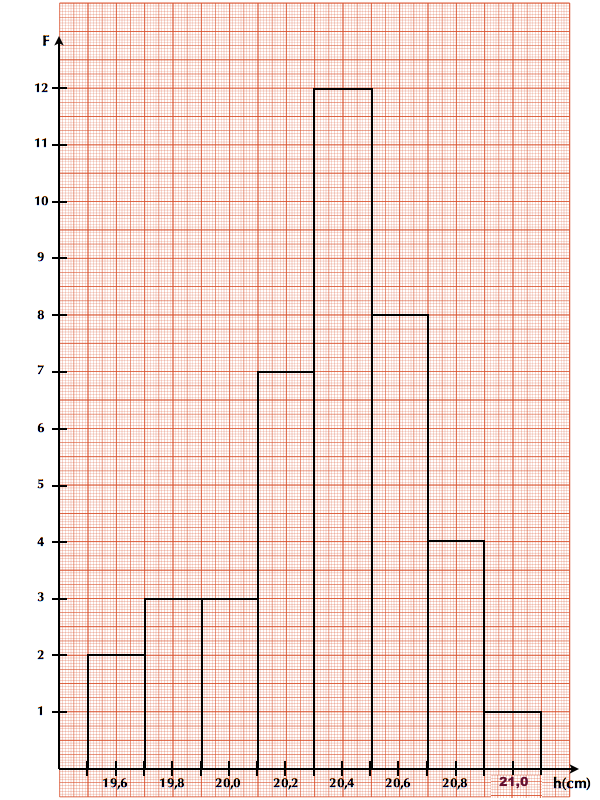
\includegraphics[width=8cm]{fig/histoH}&
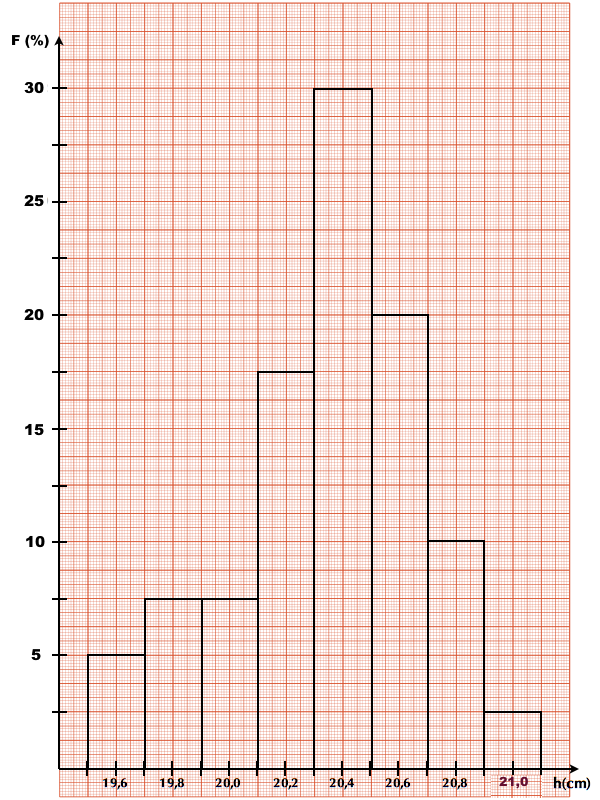
\includegraphics[width=8cm]{fig/histoHFR}\\
\end{tabular}
\caption{\label{fig:histoexemplo} Histogramas de frequências (lado esquerdo) e frequências relativas (lado direito) da medida da altura (h) da garrafa de água .}
\vspace{-1.cm}
\end{center}
\end{figure}



\section{Como construir um gráfico}\label{plot}

Uma forma muito útil de apresentar os resultados experimentais é a partir de re\-pre\-sen\-ta\-ções gráficas dos mesmos, pois neles a informação é sintetizada, facilitando sua análise e interpretação. Geralmente, um gráfico é mais útil que uma tabela de valores, por exemplo, quando estamos realizando medições de uma variável Y em função de outra X que varia independentemente e queremos ver a relação funcional entre elas (por exemplo, a posição de um móvel em função do tempo), ou para estudar se duas variáveis possuem alguma correlação ou não.

Em Física Experimental I, todos os gráficos que realizaremos serão em duas dimensões além dos histogramas que já foram discutidos na sessão~\ref{sec:histo}. O primeiro passo é escolher quais serão as variáveis e, logo, qual é a variável independente que será representada no eixo horizontal e qual a dependente no eixo vertical.  Por exemplo, se queremos representar a posição de um corpo em movimento em função do tempo vamos identificar duas variáveis:  posição ($x$) e tempo (t), sendo o tempo a variável independente.  Ou seja, o tempo será colocado no eixo-x e a posição no eixo-y. 

Uma vez escolhidas as variáveis, devemos determinar a escala para cada eixo. Para isto temos que considerar os valores medidos de cada variável, de forma a poder escolher uma escala que facilite a leitura dos pontos experimentais, ou qualquer outro ponto representado no gráfico.  Quando desenhamos o gráfico em papel, devemos escolher a escala de forma a usar pelo menos metade da folha para representar os pontos experimentais. Para facilitar a leitura do gráfico, é interessante utilizar escalas em que cada milímetro do papel corresponda a múltiplos ou submúltiplos de 2 ou 5 da grandeza correspondente. A determinação da escala em cada eixo é independente.   

Consideremos os seguintes valores medidos para o exemplo da posição do corpo em função do tempo: %(Tabela~\ref{tab:dados}).
\vspace{-0.7cm}
\begin{center}
  \begin{tabular}{|c|c|c|}
  Tempo (s) & Posição (m)  & Incerteza da Posição (m)	\\
0,1	&	29 & 1 \\
0,3	&	34 & 1 \\
0,4	&	41 & 1 \\
0,5	&	38 & 1 \\ 
0,7	&	33 & 1 \\ 
1,0	&	26 & 1 \\
1,1	&	23 & 1 \\
1,2	&	20 & 1 \\
1,4	&	17 & 1 \\
1,5	&	16 & 1 \\
\end{tabular}
%\caption{Tabela da posição em função do tempo.
%\label{tab:dados} %}
\vspace{-0.4cm}
\end{center}

Vamos construir o gráfico em papel milimetrado, usando a folha ``na vertical'', de forma que o eixo-x fique na menor dimensão da mesma e o eixo-y na maior. Para o eixo-x, onde vamos representar o tempo, a escolha parece simples, começamos em 0 (zero) e consideramos uma escala de 10 mm para cada 0,1 s, pois o tamanho nesta dimensão é de 180 mm e nós precisamos marcar de 0 a 1,5 s. Para o eixo-y, onde vamos representar a posição, dispomos de 28 cm de folha. Neste caso, podemos considerar duas possibilidades: (A) começamos a escala a partir do zero ou (B) começamos ela perto do menor valor medido, neste caso 16 m.  Em ambos  os casos a escala deve ir até o máximo valor medido ou algum valor superior imediato.  Em geral escolhemos um valor superior que permita ajustar a escala para um múltiplo de 2 ou 5. Se consideramos o caso (A), uma escala possível seria 1 cm no papel para cada 2 m de posição (Figura~\ref{fig:plots} (esquerda)). Como podemos ver, não é necessário começar do zero, podemos começar por exemplo de 15 m (caso B) e escolher uma escala de 1 cm para cada 1 m (Figura~\ref{fig:plots} (direita)). Desta forma podemos observar melhor a estrutura própria do gráfico. Uma vez definida a escala, marcamos valores regularmente espaçados nos eixos correspondentes e identificamos os eixos com as grandezas que estes representam, com suas respectivas unidades. Finalmente, desenha-se os  pontos com suas barras de erro de acordo com a tabela de dados, como pode se ver na Figura~\ref{fig:plots}. A barra de erro é a representação gráfica da incerteza. Assim, ela deve ser desenhada como uma reta que vai de um valor igual ao valor do ponto subtraído do valor de uma incerteza até o valor do ponto somado de uma incerteza.

Não existe uma única forma de representar os nossos dados.  No exemplo anterior, ambos os gráficos estão corretos. {\bf O importante é que se deve adotar uma “escala limpa e fácil de ser lida” de modo a que não seja necessário fazer cálculos para achar a localização dos pontos no gráfico. Se você precisar fazer muitos cálculos, algo está inadequado.}

\begin{figure}[t]
\vspace{0.5cm}
\begin{minipage}{\textwidth}
\begin{minipage}[t]{0.47\textwidth}
 \begin{center}
 \includegraphics*[width=0.99\textwidth]{fig/Plot1}
\end{center}
\end{minipage}
%\hspace{0.3cm}
\begin{minipage}[t]{0.47\textwidth}
\begin{center}
 \includegraphics*[width=0.99\textwidth]{fig/Plot2}
     \end{center}
   \end{minipage}
 \end{minipage}
\caption{\label{fig:plots}  Gráfico da posição (x) em função do tempo (s) para o caso A (esquerda). Gráfico da posição (x) em função do tempo (s) para o caso B (direita).}
\end{figure} 


\chapter{Ajuste linear}
\label{chap:minquad}
\section{Ajuste de uma função linear por Mínimos Quadrados}
\label{sec:minquad}


Se medimos duas variáveis, X e Y, cuja relação sabemos que é linear, podemos encontrar uma relação analítica que melhor ajuste nossos dados. A forma de realizá-la é mediante o procedimento de Mínimos Quadrados, que no caso particular de uma função linear chama-se de regressão ou ajuste linear. Em Física Experimental I, só trabalharemos com este tipo de ajuste, seja porque as relações das grandezas medidas tem uma relação linear ou porque seremos capazes de linearizar relações entre grandezas.

Vamos então nos focalizar só no caso da regressão linear, deixando o caso mais genérico de mínimos quadrados para ser estudado mais para a frente. Na Figura~\ref{fig:ajuste}, mostramos o caso linear. A dispersão dos valores está associada às flutuações dos valores de cada variável. Supomos uma tendência linear entre as variáveis X e Y, e nos perguntamos qual é a melhor reta: 
\begin{equation}
y(x) = a x + b
\end{equation}
\noindent
que ajusta estes dados. A quantidade $y_i - y(x_i)$ representa o desvio de cada medida $y_i$ em relação ao valor previsto pelo modelo $y(x)$.

\begin{figure}[h]
\begin{center}
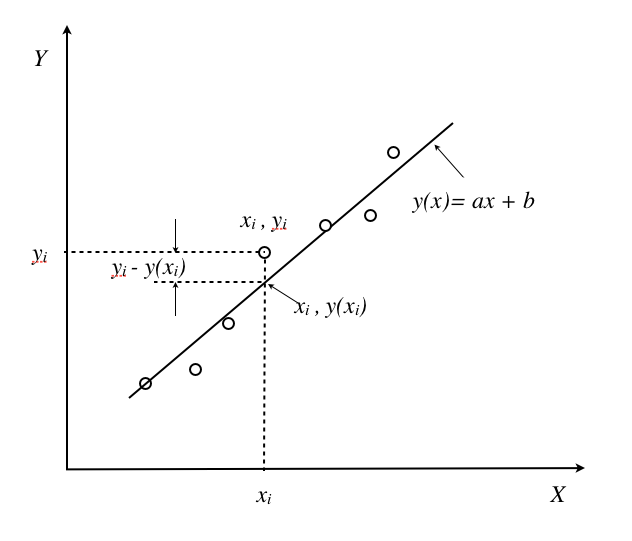
\includegraphics[width=8cm]{fig/GraficoAjusteLin}
\vspace{-0.4cm}
\caption{\label{fig:ajuste} Gráfico de dados associado a um modelo linear.}
\vspace{-1.5cm}
\end{center}
\end{figure}

Vamos definir uma função $\chi^2$ (chi-quadrado), dada por: 
\begin{equation}
\chi^2 = \sum_{i=1}^N (y_i - (ax_i + b))^2
\end{equation}
\noindent
onde $N$ é o número de pontos que serão utilizados para a realização do ajuste linear. Desta forma, a função $\chi^2$ é uma medida do desvio total dos valores medidos $y_i$ em relação aos valores previstos pelo modelo linear $ax + b$. Os melhores valores para o coeficiente angular $a$ e o coeficiente linear $b$ são os que minimizam este desvio total, ou seja o valor de $\chi^2$. Portanto, os melhores valores de $a$ e $b$ serão os que satisfazem:
\begin{equation}
\frac{\partial \chi^2}{\partial a} = 0~~~~~ \text{e}~~~~~ \frac{\partial \chi^2}{\partial b} = 0
\end{equation}

Resolvendo as duas equações obtemos (mostrar):
\begin{equation}
a = \frac{N\sum_i x_i y_i - \sum_i x_i \sum_i y_i}{N \sum_i x_i^2 - (\sum_i x_i)^2}
\end{equation}
\begin{equation}
b = \frac{\sum_i x_i^2 \sum_i y_i - \sum_i x_i \sum_i x_i y_i}{N \sum_i x_i^2 - (\sum_i x_i)^2}
\end{equation}

Estes dois resultados se aplicam ao caso em que todos os dados da variável dependente ($y$) têm a mesma incerteza absoluta e a incerteza da variável independente ($x$) considera-se desprezível. As incertezas dos parâmetros $a$ e $b$ são dadas por:
\begin{equation}
\sigma_a = \sqrt{\frac{\chi_N^2}{N~V[x]}} ~~~~~ \text{e}~~~~~ \sigma_a = \sqrt{\frac{\chi_N^2 \sum_i x_i^2}{N~V[x]}}
\end{equation}
\noindent
onde $V[x]$ é a variância de $x$ e $\chi^2_N$ é conhecido como o chi-quadrado por grau de liberdade (ou chi-quadrado reduzido), que no caso linear está dado por:
\begin{equation}
\chi^2_N = \frac{1}{N-2} \chi^2 = \frac{1}{N-2} \sum_{i=1}^N (y_i - (ax_i + b))^2
\end{equation}

A qualidade do ajuste linear pode ser determinada pelo {\it coeficiente de correlação} dado por:
\begin{equation}
\rho = \frac{\frac{1}{N} \sum_i x_i y_i - \frac{1}{N^2} \sum_i x_i \sum_i y_i}{\sqrt{V[x] V[y]}}
\end{equation}
\noindent
onde:
\begin{equation}
V[x] = \frac{1}{N} \sum_{i=1}^N x_i^2 - \left( \frac{1}{N} \sum_{i=1}^N x_i \right) ^2 ~~~ \text{e}~~~V[y] = \frac{1}{N} \sum_{i=1}^N y_i^2 - \left(  \frac{1}{N} \sum_{i=1}^N y_i \right)^2
\end{equation}



\section{Método gráfico para ajustar uma reta com incerteza}\label{retagrafico}



Se medimos duas variáveis, X e Y, cuja relação sabemos que é linear, podemos encontrar uma relação analítica que melhor ajuste nossos dados. No Capítulo ~\ref{sec:graf}  da parte Conceitos Básicos na apostila discutimos como isto é feito analiticamente mediante o método de mínimos quadrados, mas aqui estudaremos como faze-lo a partir do gráfico de Y em função de X, o que chamamos de {\bf método gráfico}.

Na Figura~\ref{fig:graflin} podemos observar a distribuição dos dados, círculos abertos, que queremos ajustar. Neste caso, para simplificar, vamos considerar que a incerteza associada a cada medida é do tamanho do ponto.  Para ajustar graficamente os pontos  por uma reta que melhor representa a variação de Y em função de X devemos traçar uma reta de forma tal que os pontos que se situem ``acima" da reta se vejam compensados pelos pontos que se situem ``abaixo'' da mesma, como na linha cheia mostrada na Figura~\ref{fig:graflin}~\footnote{Note que o uso de uma régua transparente é conveniente pois permite ter uma visão global de todos os pontos.}. 
\begin{figure}[!h]
\vspace{-0.4cm}
\begin{center}
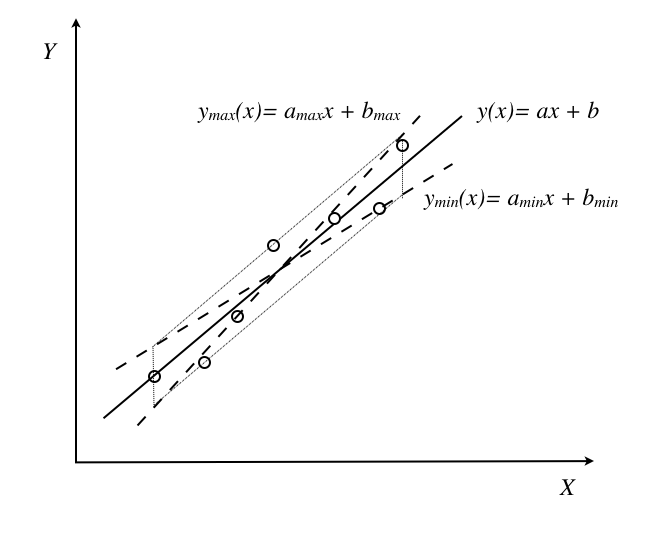
\includegraphics[width=9cm]{fig/GraficoLinGrafico}
\caption{\label{fig:graflin} Método para ajuste linear.}
\vspace{-0.4cm}
\end{center}
\end{figure}


Desta forma podemos determinar o coeficiente angular ($a$) e linear ($b$) para a equação da reta $y = ax + b$.  Mas mesmo no caso gráfico é preciso dar as incertezas associadas à determinação de $a$ e $b$.  Para isto, vamos traçar duas linhas paralelas à melhor reta ($R$) que ajusta os nossos dados encontrados, uma passando pelo ponto mais afastado ``acima'' da reta $R$ e outra pelo ponto mas afastado ``abaixo'' da reta $R$. %, formando o paralelepípedo pontilhado tal como é mostrado na figura. 
Caso exista um ou outro ponto excepcionalmente afastado da reta média poderá não ser considerado pois a probabilidade de corresponder a uma medida incorreta é grande. Obtendo a interseção destas retas por duas retas paralelas ao eixo-y que contêm o primeiro e último ponto experimental representado temos um ``paralelogramo de incerteza" como é mostrado na figura (paralelogramo pontilhado). A partir deste, desenhamos as duas retas diagonais achando o que chamaremos a reta de máxima $y_{max} = a_{max} x + b_{max}$ e a de mínima $y_{min} = a_{min} x + b_{min}$ (ver figura).

A partir destas três retas, podemos então determinar as incertezas associadas para o coeficiente angular $\delta a$ e linear $\delta b$ como:
\[
\delta a = \frac{a_{max} - a_{min}}{2} 
\]
\[
\delta b = \frac{b_{max} - b_{min}}{2}
\]


\chapter{Determinação da velocidade instantânea}
\label{sec:vinst}

No movimento uniformemente acelerado a velocidade da partícula em um instante $t$ pode ser calculada a partir da velocidade média calculada entre os instantes $t + \Delta t$ e $t - \Delta t$ com $\Delta t$ constante. Isto é:
\begin{equation}
< v(t) > = \frac{x(t+ \Delta t) - x (t - \Delta t)}{2 \Delta t}
\end{equation}
\noindent

Assim, para um conjunto de medições de posição em função do tempo, podemos calcular a velocidade em cada ponto ($i$) a partir das medições de tempo e posição do ponto posterior ($t_{i+1}$ e $x_{i+1}$) e anterior ($t_{i-1}$ e $x_{i-1}$), utilizando a fórmula: 
\begin{equation}
v_i = \frac{x_{i+1}-x_{i-1}}{t_{i+1} -t_{i-1}}
\end{equation}
\noindent

Para cada valor de velocidade também podemos calcular a incerteza associada mediante a fórmula de propagação de incertezas. Desprezando a incerteza na determinação do tempo, obtemos:\begin{equation}
\delta^2_{v_i} = \frac{\delta^2_{x_{i+1}}+\delta^2_{x_{i-1}}}{(t_{i+1} -t_{i-1})^2}
\end{equation}
\noindent
onde $\delta_{x_{i+1}}$ e $\delta_{x_{i-1}}$ são as incertezas na determinação da posição ${x_{i+1}}$ e ${x_{i-1}}$ respectivamente.



\chapter{Distribuição Gaussiana}
\label{sec:gauss}

\vspace{-0.7cm}

\section*{Valor médio, Desvio Padrão e Densidade de Probabilidade}

Sejam $N$ medições aleatórias independentes de uma grandeza qualquer, $x_1, x_2, x_3, ... , x_N$. Como alguns dos valores $x_i$ medidos podem ser repetidos, podemos dizer que para esta grandeza temos $M$ {\bf eventos} possíveis de medida tal que $M \leq N$ e eles são: $y_1, y_2, ..., y_M$. Então, podemos definir a {\bf frequência de ocorrência} do evento $y_i$ como $N(y_i)$ de forma tal que:
\begin{equation}
\sum_{i=1}^M N(y_i) = N.
\end{equation}
\noindent

Desta forma, podemos definir a {\bf frequência relativa} como a fração de eventos $y_i$ em relação ao número total de eventos $N$, dada por:
\begin{equation}
F(y_i) = \frac{N(y_i)}{N},
\label{eq:freqrel}
\end{equation}
\noindent
de forma que (mostrar):
\begin{equation}
\sum_{i=1}^M F(y_i) = 1.
\end{equation}
\noindent

Se o processo é repetido indefinidamente, ou seja, $N \longrightarrow \infty$, a frequência relativa é interpretada como a {\bf probabilidade de ocorrência} do evento $y_i$:
\begin{equation}
P(y_i) = \lim_{N \to \infty} F(y_i) = \lim_{N \to \infty} \frac{N(y_i)}{N},
\end{equation}
\noindent
e como sabemos que $0  \leq N(y_i) \leq N$, então $0  \leq P(y_i) \leq 1$.

No Capítulo~\ref{stat} da parte Conceitos Básicos definimos os conceitos de valor médio e desvio padrão. Agora podemos re-escrever estas definições em função da frequência relativa, obtendo:

\begin{enumerate}
\item {\bf Valor médio}
\begin{equation}
\bar{x} = \sum_{i = 1}^M F(x_i){x_i},
\end{equation}
\noindent

\item {\bf Variância $V[x] = \sigma^2$}
\begin{equation}
\sigma^2 = \sum_{i=1}^M (x_i - \bar{x})^2 F(x_i)
\end{equation}
\noindent
\vspace{-1.cm}
\end{enumerate}
 
%Frequentemente ocorre que num processo aleatório o valor médio para a determinação de uma grandeza pode resultar em um número muito grande de valores possíveis. A medida do período de oscilação de um pêndulo simples é um exemplo. 

Quan\-do realizamos observações experimentais utilizamos instrumentos que determinam os valores de grandezas que são continuamente distribuídas. Os resultados são truncados até o limite da precisão de medida do instrumento utilizado. Por exemplo, um cronômetro usual mede intervalos de tempo com precisão de um centésimo de segundo. Isto significa que intervalos de tempo menores que este valor não podem ser medidos com este instrumento. Assim, os resultados obtidos serão representados por um número finito de valores, mesmo que a variável observada seja contínua. Algumas vezes, o número de valores possíveis medidos, mesmo que finito, pode ser muito grande, e para estes casos é conveniente agrupa-los em intervalos.  Desta forma o conjunto de medidas diferentes fica reduzido sem que a informação da amostra original seja perdida.

Consideremos novamente $N$ medições aleatórias independentes de uma grandeza qualquer, $x_1, x_2, x_3, ... , x_N$. Para estes casos, definimos como o mesmo evento todo resultado da realização do processo aleatório $y$ que caia num intervalo de valores $\Delta y$, de forma que o evento agora será caracterizado por $\{y_i, \Delta y\}$: 
\begin{equation}
y_i - \frac{\Delta y}{2} \leq x_j  < y_i + \frac{\Delta y}{2}.
\end{equation}

A probabilidade de ocorrência do evento $\{y_i, \Delta y \}$ é definida por:
\begin{equation}
P(y_i) = \Delta P_i
\end{equation}
\noindent
onde $\Delta P_i$ é a probabilidade de encontrarmos como resultado da realização do processo aleatório, valores no intervalo $\{y_i - \frac{\Delta y}{2}, y_i +	 \frac{\Delta y}{2}\}$. Para intervalos $\Delta y$ pequenos, podemos escrever a seguinte relação:
\begin{equation}
P(y_i) = \Delta P_i = p(y_i) \Delta y
\end{equation}
\noindent
onde $p(y_i)$ é denominada de densidade de probabilidade do evento aleatório $y_i$. E se $\Delta y \longrightarrow 0$, então $\Delta P_i$ e $\Delta y$ são infinitesimais podendo escrever a densidade de probabilidade como:
\begin{equation}
p(y) = \frac{dP}{dy}
\end{equation}
\noindent
sendo que: 
\begin{equation}
\int_{-\infty}^{+\infty} \! p(y) \, \mathrm{d}y = 1
\end{equation}
\noindent

Em $N$ repetições de um processo aleatório real, a aproximação experimental para a probabilidade de realização de um evento é a frequência relativa $F(y_i)$, definida na equação~\ref{eq:freqrel}.  Assim, a densidade de probabilidade experimental $p_{exp}(y_i)$ de ocorrência do evento $\{y_i, \Delta y \}$ é dada por:  
\begin{equation}
p_{exp}(y_i) = \frac{F(y_i)}{\Delta y}.
\end{equation}
\noindent

Para o caso contínuo e utilizando o conceito de densidade de probabilidade, o valor médio ($\mu$) e a variância ($\sigma^2$) podem ser escritos da seguinte forma: 

\begin{enumerate}
\item {\bf Valor médio}
\begin{equation}
\mu = \int_{-\infty}^{+\infty} \! y~p(y) \, \mathrm{d}y. 
\end{equation}
\noindent

\item {\bf Variância $V[y] = \sigma^2$}
\begin{equation}
\sigma^2 =\int_{-\infty}^{+\infty} \! (y-\mu)^2~p(y) \, \mathrm{d}y. 
\end{equation}
\end{enumerate}



\section*{Função de Laplace-Gauss}

Em muitas situações experimentais utilizamos {\bf distribuições Gaussianas} para interpretar nossos resultados físicos, em parte porque os fundamentos teóricos das medições realizadas se correspondem com distribuições Gaussianas ou porque a experiência tem nos mostrado que a estatística de Gauss nos proporciona uma descrição razoavelmente acurada dos vários eventos reais. Na distribuição Gaussiana, a densidade de probabilidade é dada por:
\begin{equation}
p(x) = G(x) = \frac{1}{\sqrt{2 \pi \sigma^2}}~e^{-\frac{1}{2}\left(\frac{x - \mu}{\sigma}\right)^2}
\label{eq:gauss}
\end{equation}
\noindent
onde $\mu $ é o valor médio e $\sigma$ o desvio padrão da distribuição, dados pelas equações discutidas anteriormente.

Na Figura~\ref{fig:gauss} apresentamos a função Gaussiana de densidade de probabilidade para a variável continua $x$.  Esta função é também chamada de função de Laplace-Gauss ou função Normal. O gráfico da função Gaussiana é uma curva simétrica em forma de ``sino'' \-com uma altura máxima dada por $G_{max} = 1/\sqrt{2 \pi \sigma^2}$. Pode ser mostrado a partir da equação~\ref{eq:gauss} que 
$\sigma$ é a meia largura da curva na altura correspondente a $\sim 0,61 G_{max}$ e que a área sob a curva entre $\mu - \sigma$ e $\mu + \sigma$ (região pintada na Figura~\ref{fig:gauss}) corresponde a 68,3\% da área total. Isto quer dizer que a probabilidade de medirmos um valor no intervalo $\mu \pm \sigma$ é 68,3\%. Seguindo o mesmo procedimento, podemos mostrar que a probabilidade de encontrarmos um valor entre  $\mu \pm 2\sigma$ é 95,4\% e entre $\mu \pm 3\sigma$ é 99,7\%.


\begin{figure}[t]
\begin{center}
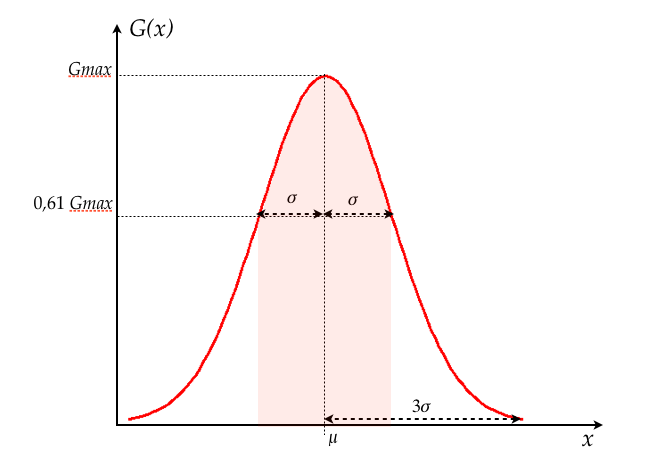
\includegraphics[width=14cm]{fig/Gauss.png}
%\vspace{-0.7cm}
\caption{\label{fig:gauss} Representação da função Gaussiana.}
\end{center}
%\vspace{13cm}
\end{figure}


%\let\clearpage\relax
%\chapter{Referências}
%\label{sec:referencias_bibliograficas}
\vspace{-0.7cm}

\begin{thebibliography}{9}
\bibitem{Vuolo} Fundamentos da Teoria de Erros,  José Henrique Vuolo,  $2.^a$ Edição 1996, Editora Edgar Blücher Ltda,

\bibitem{Moyses} Curso de Física Básica,  – Mecânica Volume 1), H. Moysés Nussenzveig, $2.^a$ Edição 2015, Ed. Edgard Blücher Ltda,

\bibitem{SearsZemansky} Física I – Mecânica, Sears \& Zemansky / Young \& Freedman, $14.^a$ Edição 2016, Pearson Education do Brasdil Ltda., 

\bibitem{Galante2020}
{\it Two-penny physics: Teaching 2D linear momentum conservation}, 
L. Galante e I. Gnesi, 
American Journal of Physics {\bf88}, 279  (2020).

\bibitem{deJesus2016}
{\it Uma visão diferenciada sobre o ensino de forças impulsivas
usando um smartphone}, 
V. L. B. de Jesus e D. G. G. Sasaki, 
Revista Brasileira de Ensino de Física {\bf38}, 1303  (2016).
\end{thebibliography}


%\chapter{Referências}
%\chapter{Bibliografia}

%\label{sec:referencias_bibliograficas}
\vspace{-0.7cm}

\begin{thebibliography}{9}
\bibitem{Vuolo} Fundamentos da Teoria de Erros,  José Henrique Vuolo,  $2.^a$ Edição 1996, Editora Edgar Blücher Ltda,

\bibitem{Moyses} Curso de Física Básica,  – Mecânica Volume 1), H. Moysés Nussenzveig, $2.^a$ Edição 2015, Ed. Edgard Blücher Ltda,

\bibitem{SearsZemansky} Física I – Mecânica, Sears \& Zemansky / Young \& Freedman, $14.^a$ Edição 2016, Pearson Education do Brasdil Ltda., 

\bibitem{Galante2020}
{\it Two-penny physics: Teaching 2D linear momentum conservation}, 
L. Galante e I. Gnesi, 
American Journal of Physics {\bf88}, 279  (2020).

\bibitem{deJesus2016}
{\it Uma visão diferenciada sobre o ensino de forças impulsivas
usando um smartphone}, 
V. L. B. de Jesus e D. G. G. Sasaki, 
Revista Brasileira de Ensino de Física {\bf38}, 1303  (2016).
\end{thebibliography}


%\cite{Moyses}
%Da Mariana 10.09.2020
%\bibliographystyle{IEEEtran}
%\bibliography{/Users/soeiros/Documents/MESTRADO/Mestrado-2020/Dissetacao-Mestrado-2020/abntex2-options.bib}
%
%\input{Capitulo1}\caption{\label{fig4AppB} Movimentando os ícones pretos indicados pelas setas verde e laranja escolhemos os quadros iniciais e finais respectivamente.}
%\let\cleardoublepage\clearpage
%\input{Capitulo2}
%\input{Capitulo3}
%\input{Capitulo4}
%\input{Capitulo5}

%%\part{Exercícios}
%\setcounter{chapter}{0}
%%\chapter{Algarismos significativos}

\vspace{-0.7cm}

Expresse corretamente os resultados para as seguintes medições com suas respectivas incertezas.

\begin{center}
\vspace{-1cm}
  \begin{tabular}{|c | c | c | c |>{ \centering\arraybackslash}m{8cm} |}  \hline
    & Medição	& Incerteza	& Unidades	& Resultado \\ \hline	 	
    1 & 67,002 & 0,023 & cm & \\ \hline
2 & 0,001 & 2,3 & erg & \\ \hline
3 & 45612,98 & 345 & cm/s & \\ \hline
4 & 14 & 29 & erg & \\ \hline
5 & 152,389 & 0,037 & cm/s$^2$ & \\ \hline
6 & 74,58 & 3,14 & g & \\ \hline
7 & 0,0012 & 0,0001 & m & \\ \hline
8 & 120034 & 2607 & m/s$^2$ & \\ \hline
9 & 45,98 & 2,1 & erg & \\ \hline
10 & 65555,467 & 56,001 & g & \\ \hline
11 & 23,456 & 1,2 & m & \\ \hline
12 & 0,173 & 0,056 & cm$^3$ & \\ \hline
13 & 45001,6 & 657,31 & J & \\ \hline
14 & 45,629 & 2,5914 & km/h & \\ \hline
15 & 104104 & 104 & m$^2$ & \\ \hline
16 & 0,0826 & 0,099 & cm/s & \\ \hline
17 & 3,69 & 1,582 & mm$^3$ & \\ \hline


    
  \end{tabular}
\end{center}


\begin{center}
  \begin{tabular}{|c | c | c | c |>{ \centering\arraybackslash}m{8cm} |}  \hline
    & Medição	& Incerteza	& Unidades	& Resultado \\ \hline	 

18 & 19,78 & 5,46 & kg & \\ \hline
19 & 0,458 & 0,177 & cm & \\ \hline
20 & 135,589 & 0,0888 & g & \\ \hline
21 & 25,36 & 0,84 & cm & \\ \hline
22 & 74589,589 & 5698,26 & erg & \\ \hline
23 & 0,145 & 0,5 & cm/s & \\ \hline
24 & 14580,8 & 37,36 & erg & \\ \hline
25 & 125,369 & 0,041 & cm/s$^2$ & \\ \hline
26 & 74,58 & 3,14 & g & \\ \hline
27 & 0,025 & 0,0074 & m & \\ \hline
28 & 256 & 0,5 & m/s$^2$ & \\ \hline
29 & 7489 & 2,1 & m/s$^2$ & \\ \hline
30 & 4789,4 & 36,001 & g & \\ \hline
  \end{tabular}
\end{center}


%%\chapter{Propagação incerteza}

\vspace{-0.7cm}

\begin{num}

\item Os lados de um paralelepípedo são $a$ = (4,50 $\pm$ 0,05) cm, $b$ = (8,50 $\pm$ 0,09)~cm e $c$ = (35,0 $\pm$ 0,3) mm. Determinar o volume do cubo com sua incerteza absoluta e relativa.

\item Na medição da resistência (R), se obteve o valor da tensão V = (15,2 $\pm$ 0,2)~V e da corrente I = (2,6 $\pm$ 0,1)~A. Qual é a incerteza absoluta da resistência usando a equação R = V/I?
 
\item Um pêndulo simples é utilizado para medir o valor da aceleração da gravidade utilizando equação:

\[ 
T = 2 \pi \sqrt{\frac{l}{g}}.
\]
\noindent
O período $T$ medido foi de (1,24 $\pm$ 0,02)~s e o comprimento do pêndulo $l$ = (0,381 $\pm$ 0,002)~m. Qual é o resultado do valor da aceleração da gravidade $g$ com sua incerteza absoluta e relativa?

\item Para medir o comprimento total de um pêndulo (fio + esfera) usou-se uma régua milimetrada para medir o comprimento do fio e um paquímetro para medir o diâmetro da esfera. Observam-se os seguintes valores com as suas respectivas incertezas: 
\begin{iten}
\item[ ]Comprimento do fio = 2,100 m			
\item[ ] Incerteza comprimento do fio = 0,5 cm
\item[ ]Diâmetro da esfera = 2,114 cm			
\item[ ] Incerteza do diâmetro da esfera = 0,01 mm
\end{iten}
\noindent 
Ache o comprimento total e a sua incerteza associada.

\item Para o cálculo do volume de uma esfera, foi dado o raio da mesma: R = (232,0 $\pm$ 0,1)~mm. Calcular seu volume com a sua respectiva incerteza relativa.

\item A partir da figura~\ref{fig:fig1}, com as seguintes medidas:
\begin{iten}
\item[ ] L1 = (5,00 $\pm$ 0,05) cm
\item[ ] L2 = (20,00 $\pm$ 0,05) mm
\item[ ] L3 = (15,00 $\pm$ 0,01) mm
\end{iten}
\begin{figure}[t]
\begin{center}
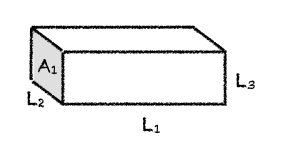
\includegraphics[width=8cm]{fig/Fig1}
\caption{\label{fig:fig1} Bloco retangular.}
\vspace{-0.4cm}
\end{center}
\end{figure}
\begin{num}
\item Determine a área A1 com a incerteza correspondente.
\item Determine o volume desta peça com a incerteza correspondente.
\item Se a precisão necessária para o resultado da área é de 0,5\% podemos considerar este resultado satisfatório?
\end{num}

\item Para determinar a altura de uma cachoeira, algumas pessoas mediram o tempo de queda de pedrinhas que eram soltas, em queda livre, de um mesmo local. Conhecendo o tempo de queda $t$, pode-se calcular a altura $h$ a partir da relação cinemática $h = 1/2 g t^2$ em que $g$ é a aceleração da gravidade. Foi utilizado um cronômetro com precisão de centésimos de segundo e os valores $t_i$ obtidos em 8 medidas estão na seguinte tabela:

\begin{center}
  \begin{tabular}{|>{ \centering\arraybackslash}m{1cm}  |>{ \centering\arraybackslash}m{2cm} |}  \hline
    	& t(s)	 \\ \hline	 	
  1	& 1,30\\ \hline	 
2	&1,09\\ \hline	 
3	&1,03\\ \hline	 
4	&1,27\\ \hline	 
5	&1,18\\ \hline	 
6	&1,31\\ \hline	 
7	&1,24\\ \hline	 
8	&1,15\\ \hline	 
  \end{tabular}
  \end{center}

Considerando $g = (9,784 \pm 0,001)$~m/s$^2$, calcule a altura da cachoeira e a sua incerteza.

\end{num}

%\input{EE3}
%\input{EE4}

%\setcounter{chapter}{0}

\part{Apêndices}
\appendix 
\chapter{Caderno de laboratório}

\vspace{-0.7cm}

\begin{enumerate}
\item {\bf É um documento.} Nele se tem todos os registros cronológicos de um experimentos ou ideia. Portanto, deve ter datas, sem rasuras nem espaços em branco, sem inserções e se possível assinado por quem realizou as anotações.

\item {\bf É pessoal}. Pode haver outros cadernos de uso compartilhado, por exemplo, para equipamentos ou instrumentos de laboratório, etc., onde se registram informações de uso geral, como mudanças introduzidas em configurações experimentais ou estado de conservação dos equipamentos. Mas o caderno de laboratório contem ideias, propostas e modo de colocar a informação que são pessoais, próprias de cada pessoa.

\item {\bf É um registro de anotação em sequência.} Não se devem intercalar resultados nem se corrigir o que está escrito. Em caso de se detectar um erro, se anota na margem o erro encontrado e a página na qual se corrige. Isto permite saber se o erro pode-se voltar a encontrar e a partir de que dados foi corrigido. Por este mesmo motivo não se deve escrever a lápis.

\item {As páginas devem ser numeradas.} Isto permite fazer referência de forma fácil e organizada às anotações anteriores, assim como também indicar na margem onde se corrigem os erros.

\item {As fórmulas e figuras devem ter uma numeração consistente e interna.} Um exemplo prático é numerar todas as fórmulas dentro de cada página ou folha e citá-las por página–fórmula. É importante numerar todas as fórmulas, pois não sabemos no futuro qual necessitaremos citar ou utilizar.

\item {Referências completas.} No caso em que se deva utilizar uma referência externa (roteiro do experimento, artigo, livro, etc.), esta referência deve ser completa. Se uma referência é citada com frequência pode-se utilizar a última página do caderno para registrá-la e citá-la por seu número. Quando citamos alguma coisa, sempre acreditamos que vamos nos lembrar de onde saiu, mas isto só é assim a curto prazo.

\item {\bf Deve-se escrever todos os resultados.} Indicar sempre a maior quantidade de in\-for\-ma\-ção possível do experimento. Todas as condições experimentais devem ser corretamente registradas e deve-se utilizar diagramas claros das configurações experimentais e indicando também cada vez que há uma mudança. Um dado ou informação que hoje parece irrelevante em função do nosso modelo da realidade, pode resultar vital ao descobrir que nossas ideias estavam erradas ou eram incompletas. A falta de um dado de aparência menor pode invalidar tudo o que foi  realizado.

\item {\bf Deve-se escrever o plano.} O que é que se pretende medir, o que é que se procura e as considerações ou razões pelas quais se faz o experimento. O planejamento do experimento e as ideias a serem realizadas devem ser explícitas. A anotação sequencial permite seguir a evolução das idéias, dado vital também para interpretar os resultados, pois os preconceitos condicionam o que se mede e como se mede. Saber o que se pensava no momento de medir vai nos indicar se nesse momento tivemos uma determinada precaução que depois demostrou ser fundamental.

\item {\bf Deve-se escrever as conclusões.} O mesmo vale para o planejamento do experimento.

\item {\bf Fazer uma reorganização periódica das ideias.} Se uma ideia tem evoluído desde o inicio do experimento, é conveniente periodicamente fazer um quadro da situação, passando a limpo o que foi feito, para não ter que reconstruir a história a cada vez.

\end{enumerate}
\chapter{Como escrever um relatório?}
\label{sec:relatorios}
\vspace{-0.7cm}

A idéia desta nota é dar aos alunos de Física Experimental I algumas dicas e re\-co\-men\-da\-ções de como escrever um relatório. Infelizmente, não existe uma “receita” para isto, pois há várias maneiras de fazer um relatório, dependendo do tipo de trabalho realizado e de quem o escreva. Portanto, a organização do relatório pode ser diferente apresentando diferentes distribuições de seções. Nesta nota propõe-se uma estrutura básica com algumas sugestões, mas será com a experiência, com a prática e com as sucessivas correções do professor que os alunos aprenderão a fazê-lo. Escrever um relatório é um aprendizado que se obtém aos poucos.
 
O ponto principal a ser tido em conta é que no relatório deve-se apresentar os resultados obtidos de forma clara e concisa. Para isto, deve-se expor cuidadosamente quais são os objetivos do trabalho realizado, os conceitos físicos básicos necessários para a realização do experimento e como ele foi realizado, entre outros. O relatório tem que ser escrito de modo que um leitor que nunca tenha realizado o experimento descrito, ou a pesquisa realizada, seja capaz de entender e até reproduzir o trabalho a partir do conhecimento adquirido na sua leitura. Para começar, sugere-se a seguinte distribuição:

\begin{itemize}
\item {\bf Título e autores:}  O título deve descrever claramente o conteúdo do trabalho. O relatório tem que ter o(s) nome(s) do(s) autor(es) e as informações relevantes referentes a ele(s). 

\item {\bf Resumo:} Deve dar uma visão completa do trabalho realizado. De forma breve, deve-se descrever qual é o objetivo do mesmo, o que foi feito e qual foi o resultado obtido. 

\item {\bf Introdução:} 
Nela expõem-se as motivações do trabalho e os objetivos a serem atingidos. Deve-se apresentar uma revisão da informação existente sobre o tema em questão. Também, deve-se incluir uma explicação teórica mínima (não copiada de livro, mas elaborada pelos alunos) que permita a compreensão do trabalho e como esta informação está aplicada ao experimento específico. 

\item {\bf Método experimental ou Descrição do experimento:} 
Deve-se descrever em detalhe a configuração experimental utilizada, os métodos utilizados para a realização das medições, incluindo a fundamentação física. Deve-se realizar uma descrição dos aspectos relevantes dos dispositivos e equipamentos utilizados, especificando suas características importantes (precisão dos instrumentos, intervalos de medição, etc). Pode-se representar esquematicamente o dispositivo empregado para a realização do experimento de forma a acompanhar as explicações e facilitar a compreensão do leitor. 

\item {\bf Resultados e discussão: }
Esta seção tem que ser uma continuação natural da In\-tro\-du\-ção e do Método experimental ou Descrição do experimento. Deve-se incluir tabelas dos dados colhidos junto com as suas incertezas e a explicação de como foram avaliadas essas incertezas. Também deve ser realizada uma descrição de como a análise de dados foi realizada e como os resultados foram obtidos. Deve-se incluir também gráficos, junto com as curvas de ajuste dos dados realizados.  Além da análise dos dados, é fundamental realizar uma discussão dos mesmos: sua validade, precisão e a sua interpretação. Dependendo do caso, pode-se realizar uma proposição de um modelo para a descrição dos resultados ou realizar uma comparação com o modelo teórico já discutido na introdução. Caso seja necessária a utilização de equações, elas devem estar explicitadas ou, se já foram introduzidas anteriormente (na introdução), através de uma referência ao número de equação correspondente. 

Levar em conta que, dependendo do relatório e do trabalho apresentados, pode-se separar esta seção em duas independentes, uma de resultados e outra de discussões. 

Figuras e tabelas: cada figura ou tabela deve estar numerada e deve conter uma legenda ao pé que permita entendê-la. A descrição detalhada da figura deve estar incluída também no texto e referenciada pelo número. Os gráficos são considerados figuras, então deverão ser numerados de forma correlacionada com as mesmas.

\item {\bf Conclusões:} 
Deve conter uma discussão de como a partir dos resultados obtidos mostra-se que as hipóteses e objetivos do trabalho foram satisfeitos ou não. Espera-se que a discussão do trabalho seja feita de forma crítica podendo-se propor melhoras ao trabalho realizado, tanto na metodologia empregada quanto nas propostas para ampliar o objetivo do experimento no futuro.

\item {\bf Referências:} 
Deve-se informar a bibliografia citada durante o desenvolvimento do trabalho. A bibliografia pode estar relacionada ao modelo teórico discutido, a referências de equipamento utilizado, ou a artigos de referência no qual o trabalho foi baseado.

\item {\bf Apêndice:} 
Caso seja necessário, pode-se anexar um ou mais apêndices com in\-for\-ma\-ção complementar que ajude a esclarecer o conteúdo das partes anteriores (cálculos realizados para obter um dado resultado, estimativa de incertezas, etc.), mas que no corpo principal do relatório desviariam a atenção do leitor. No(s) a\-pên\-di\-ce(s) coloca-se geralmente informação adicional necessária, mas não fundamental.

\end{itemize}

\chapter   {Movimento Retilíneo Uniformemente Variado (MRUV)}
\label{sec:mruv}
\vspace{-0.7cm}

Se a força resultante sobre uma partícula de massa $m$ for, $\vec{F}$, a  segunda lei de Newton diz que:
\begin{equation}
\label{eqA1}
\vec{F}=m\vec{a},
\end{equation}
com $\vec{a}$ sendo o vetor aceleração da partícula. No caso de $\vec{F}$ ser uma força constante,
{\it viz.} não depende nem do tempo, nem da posição da partícula e nem da velocidade da mesma, da Eq.(\ref{eqA1}) vemos que 
a aceleração $\vec{a}$ é constante. Assim, a Eq.(\ref{eqA1}) pode ser facilmente integrada para obtermos:
\begin{equation}
\label{eqA2}
\int_{t_0}^{t}\vec{F}dt=m\int_{t_0}^{t} \vec{a}dt\Longrightarrow \vec{F}(t-t_0)=m(\vec{v}-\vec{v}_0)
\Longrightarrow \vec{v}=\vec{v}_0+\frac{\vec{F}}{m} (t-t_0),
\end{equation}
com $\vec{v}:=\vec{v}(t)$ e $\vec{v}_0:=\vec{v}(t_0)$.
Integrando temporalmente mais uma vez ambos os membros da Eq.(\ref{eqA2}) obtemos:
\begin{equation}
\vec{r}=\vec{r}_0+\vec{v}_0(t-t_0)+\frac{1}{2}\frac{\vec{F}}{m}(t-t_0)^2,
\end{equation}
com $\vec{r}:=\vec{r}(t)$ sendo a posição da partícula como função do tempo e 
$\vec{r}_0:=\vec{r}(t_0)$ a sua posição inicial.
\par
Vamos supor agora que a força resultante 
$\vec{F}$ é paralela à velocidade inicial $\vec{v}_0$. Como a soma vetorial de vetores paralelos 
continua sendo um vetor na mesma direção que os vetores somados, de acordo com a Eq.(\ref{eqA2}), a velocidade $\vec{v}(t)$ é paralela a $\vec{v}_0$ para todo tempo. Portanto trata-se 
de um movimento retilíneo. Como também a aceleração é constante o movimento se denomina 
Movimento Retilíneo Uniformemente Variado (MRUV). Sem perda de generalidade podemos 
chamar de eixo ``$y$'' o eixo coordenado na direção de movimento,  e as equações de movimento,  Eqs.(\ref{eqA1}) e (\ref{eqA2}), nessa direção são:
\begin{eqnarray}
y&=&y_0+v_{y0}(t-t_0) +\frac{1}{2} \frac{F}{m}(t-t_0)^2,\\
v_y&=&v_{y0}+\frac{F}{m}(t-t_0),
\end{eqnarray}
com $y:=y(t)$ e $v_y:=v_y(t)$ e as condições iniciais, $y_0:=y(t_0)$ e $v_{y0}:=v_y(t_0)$.




\chapter{Tutorial básico de uso do aplicativo Tracker}
\label{sec:tracker}
\vspace{-0.7cm}

Uma vez baixada a versão do aplicativo Tracker para o sistema operacional de seu computador, 
a partir do  endereço eletrônico  \href{https://physlets.org/tracker/}{\textcolor {blue}
{https://physlets.org/tracker/}}, instale-o seguindo as orientações no próprio sítio da Internet. Com o aplicativo instalado, siga os sete  passos descritos a seguir para realizar a tomada de dados.

\underline{\bf Passo 1:} {\bf Escolha de idioma português}\\
\vskip -0.5cm

Abra o aplicativo e no caminho Edit $>$ Language $>$ e escolha a opção português como mostra a Figura~\ref{fig1AppB}.

\underline{\bf Passo 2:} {\bf Abertura do arquivo do vídeo a ser analisado}\\
\vskip -0.5cm

Para abrir o arquivo do tipo vídeo  gravado com o celular faça um ``click'' na aba
``Arquivo'' e logo na aba ``Abrir''. Na janela que abrirá procure onde o arquivo   do tipo vídeo
está guardado e faça ``click'' nele. O Tracker carrega vídeos de quase todos os formatos gravados 
por celulares mas os arquivos não podem ser muito grandes (o arquivo carregado nas figuras 
deste tutorial era de 1,3 MB). Se o arquivo não abre tente reduzir o tamanho dele editando 
o vídeo no celular, cortando as partes em que a bolinha não se move, antes da queda, ou quando
já está no chão.
Na Figura~\ref{fig2AppB} vemos um vídeo já aberto para análise.
 \begin{minipage}{\linewidth}
      \centering
      \begin{minipage}{0.4\linewidth}
          \begin{figure}[H]
              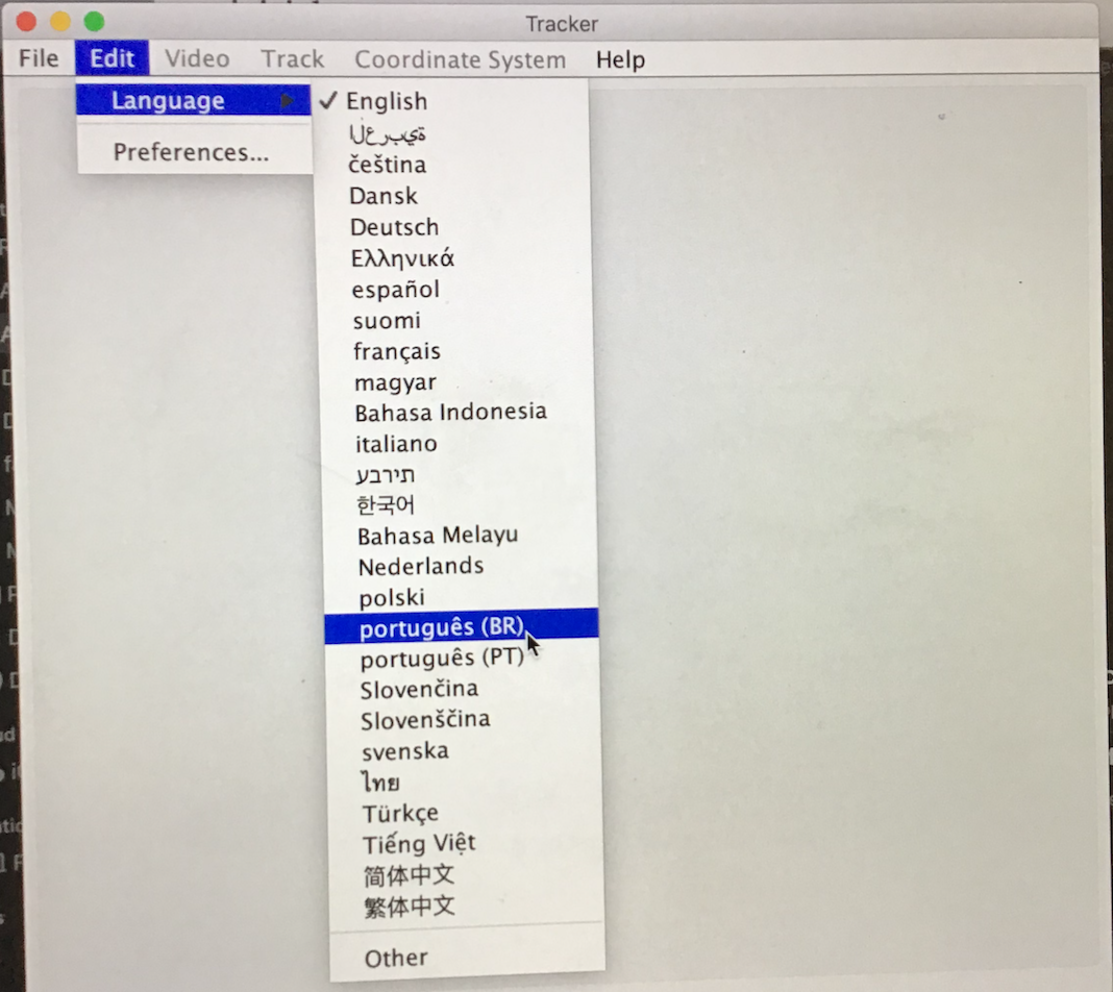
\includegraphics[width=\linewidth]{Figuras_exp3/fig1AppB.pdf}
              \caption{\label{fig1AppB} Escolha de idioma no aplicativo Tracker.}
          \end{figure}
      \end{minipage}
      \hspace{0.01\linewidth}
      \begin{minipage}{0.4\linewidth}
          \begin{figure}[H]
              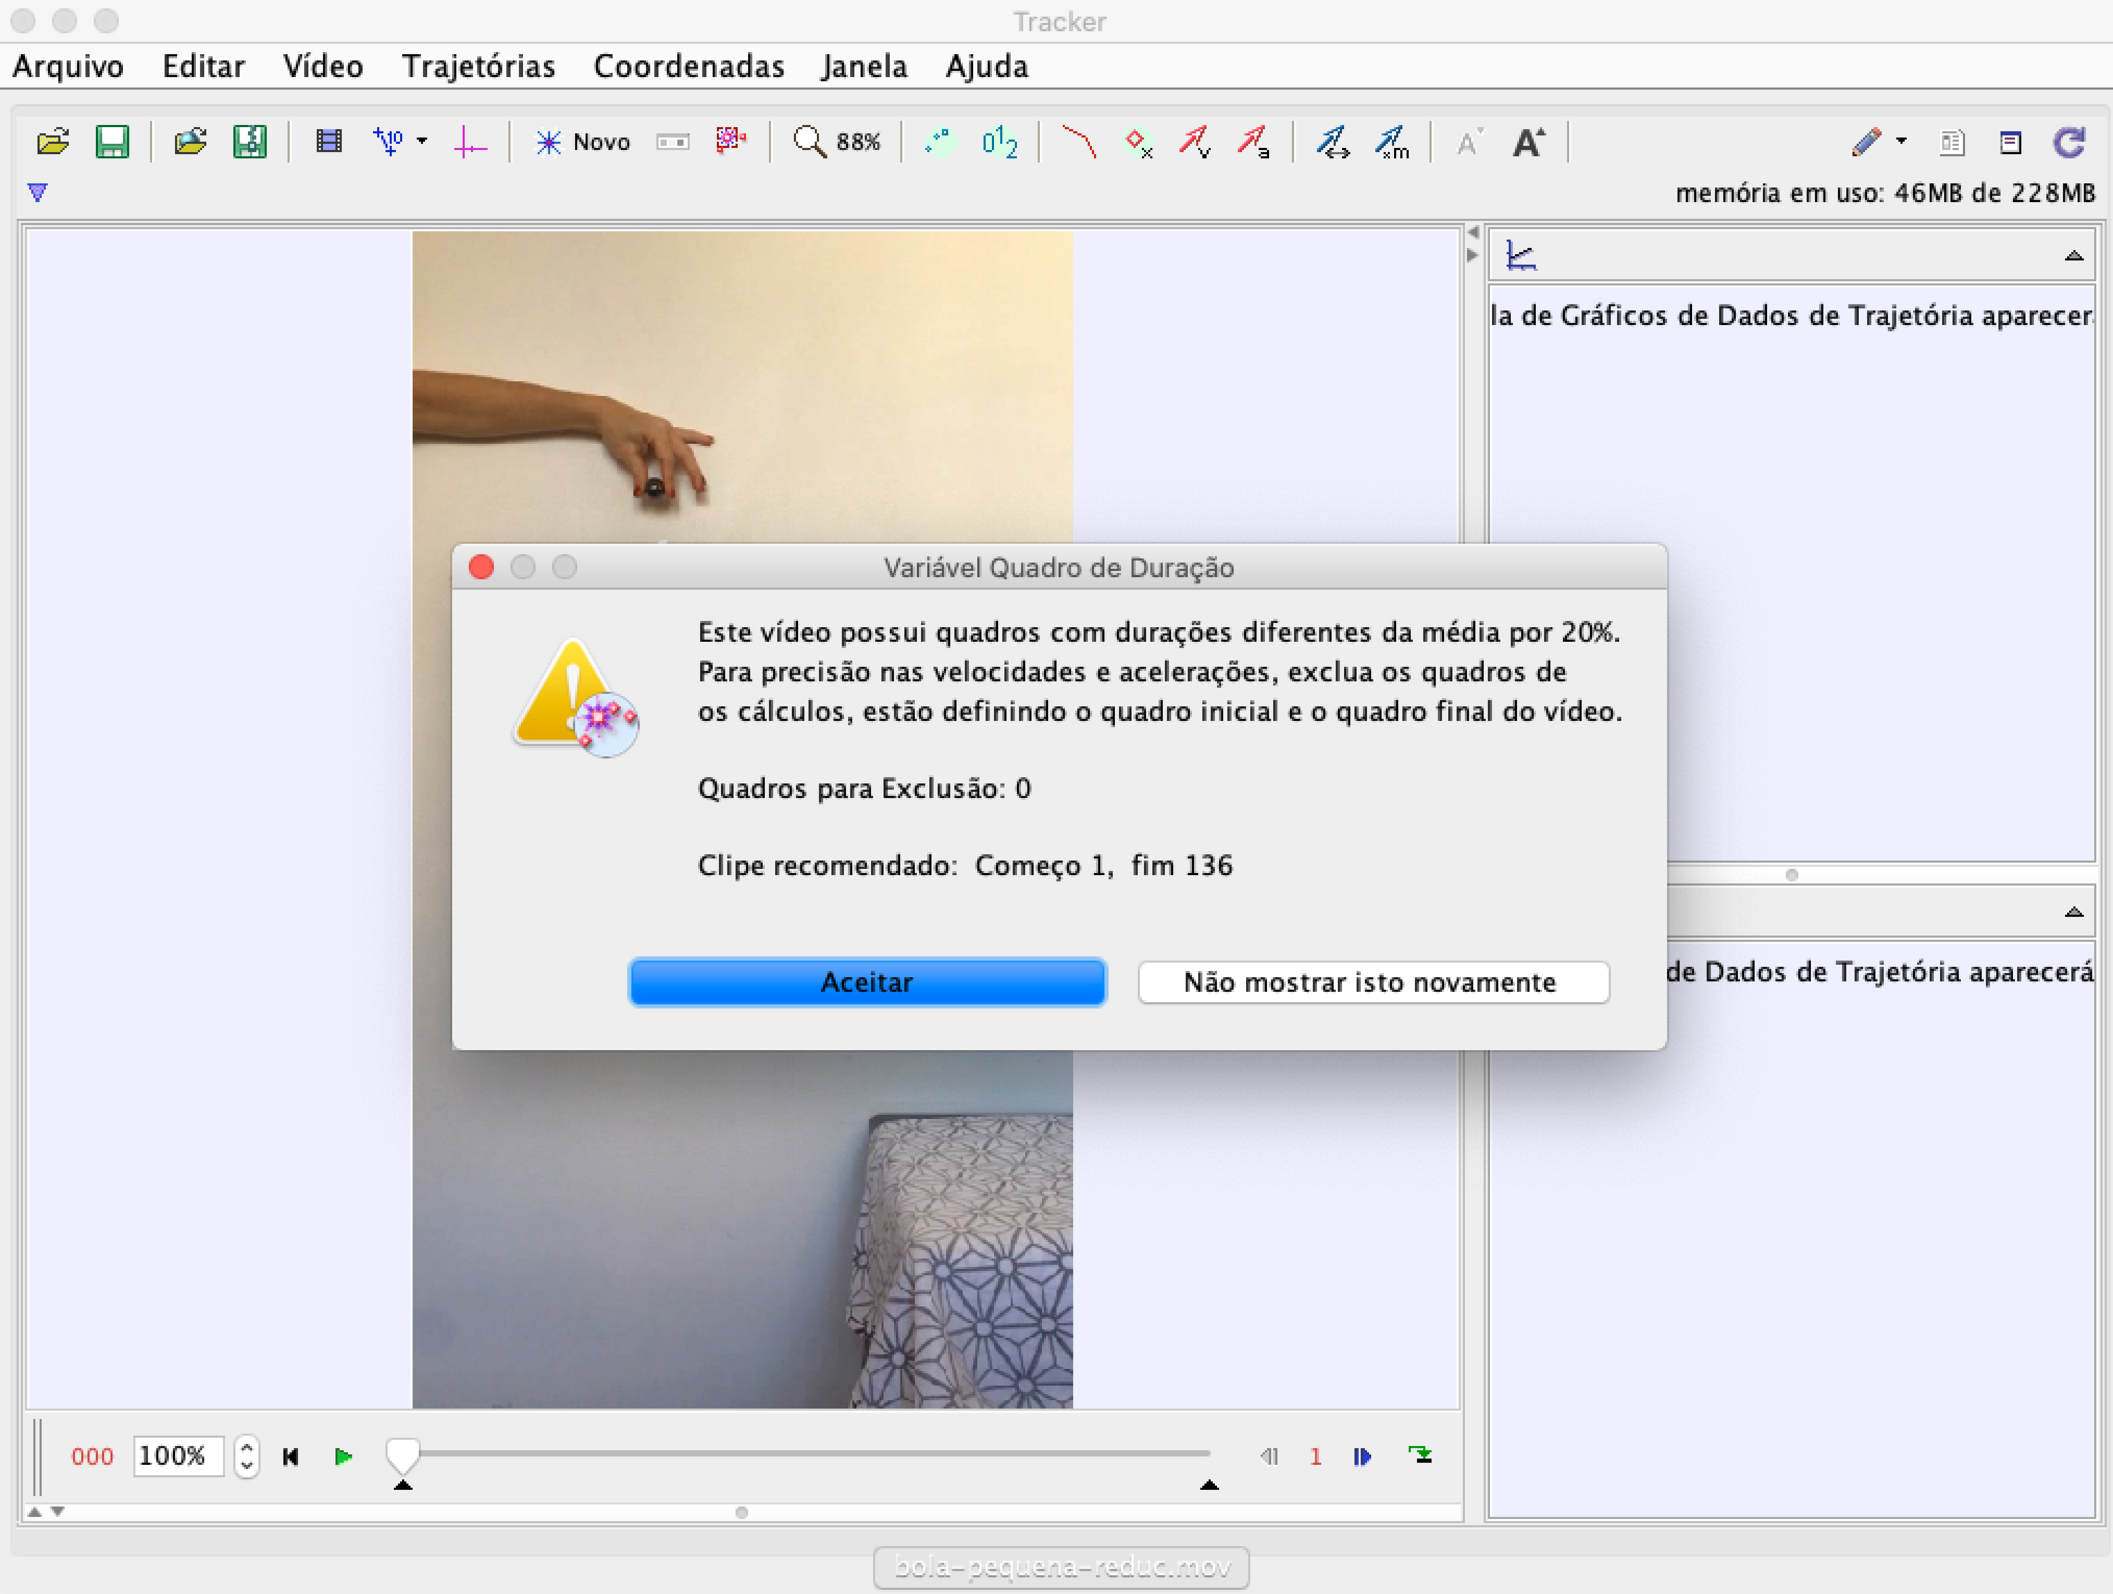
\includegraphics[width=\linewidth]{Figuras_exp3/fig2AppB.pdf}
             \caption{\label{fig2AppB} Ignore a mensagem na janela fazendo ``click em ``Aceitar''.}
          \end{figure}
      \end{minipage}
  \end{minipage}%

\underline{\bf Passo 3:} {\bf Determinação dos quadros inicial e final da análise}\\
\vskip -0.5cm

Faça ``click'' no ícone indicado pela seta preta na Figura~\ref{fig3AppB} para abrir a janela de 
``Ajustes de Corte de Vídeo''. Muitas vezes no lugar assinalado com uma seta vermelha na Figura
\ref{fig3AppB} aparece um valor muito próximo de $30.00/$s (trinta quadros por segundo), apague o valor e coloque exatamente  $30.00/$s.

As setas verdes e laranja da Figura~\ref{fig3AppB} mostram os lugares onde deveremos 
colocar os valores numéricos corretos dos quadros iniciais e finais respectivamente.
Para escolher o quadro inicial correto movimente o ícone preto indicado pela seta verde na Figura 
\ref{fig4AppB} até ver a bolinha justo saindo da mão. Verá que o valor numérico do quadro inicial 
se coloca automaticamente no lugar indicado pela seta verde na Figura~\ref{fig3AppB}. Para escolher 
o quadro final faça o mesmo com o ícone preto indicado pela seta laranja na  Figura~\ref{fig4AppB}. Escolha o quadro final mais o menos como no instante mostrado na  Figura~\ref{fig4AppB}.
Finalmente feche a janela ``Ajustes de Corte de Vídeo'' fazendo ``click em ``Aceitar''.

  \begin{minipage}{\linewidth}
  \centering
  \begin{minipage}{0.4\linewidth}
          \begin{figure}[H]
              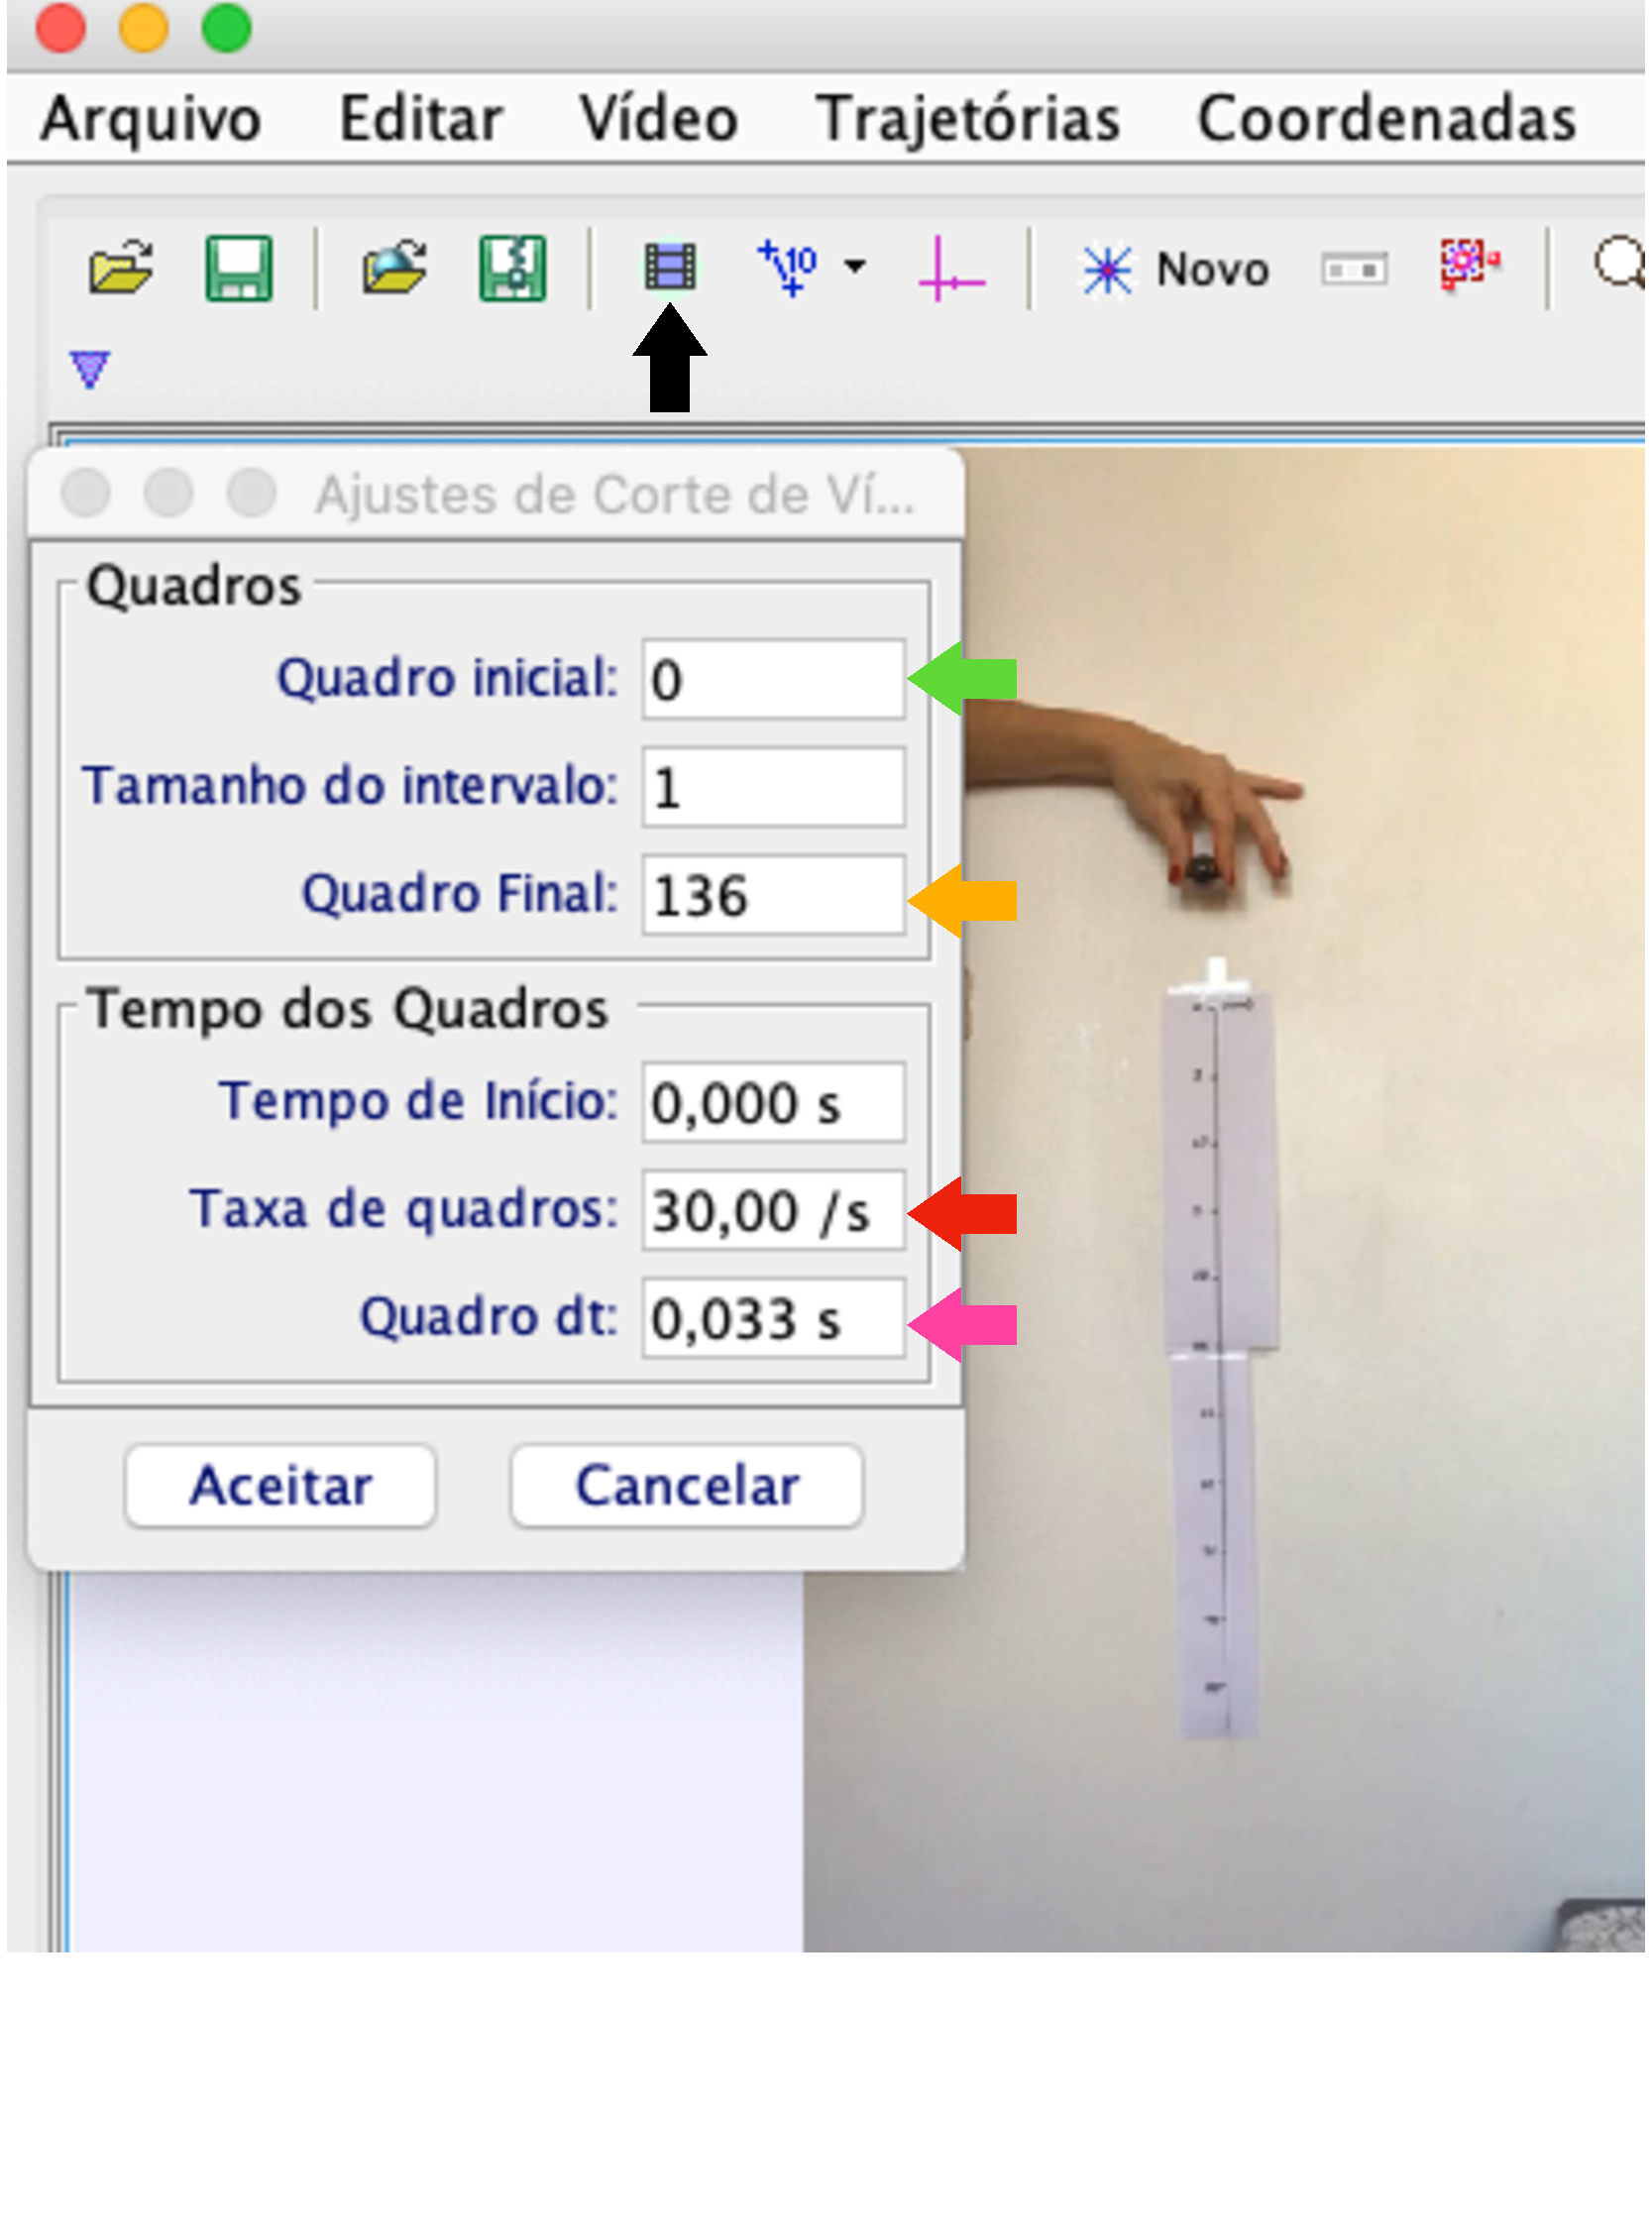
\includegraphics[width=\linewidth]{Figuras_exp3/fig3AppB.pdf}
\caption{\label{fig3AppB} Faça ``click'' no ícone indicado pela seta preta para abrir a janela de 
``Ajustes de Corte de Vídeo''.}
          \end{figure}
      \end{minipage}
      \hspace{0.01\linewidth}
      \begin{minipage}{0.43\linewidth}
          \begin{figure}[H]
              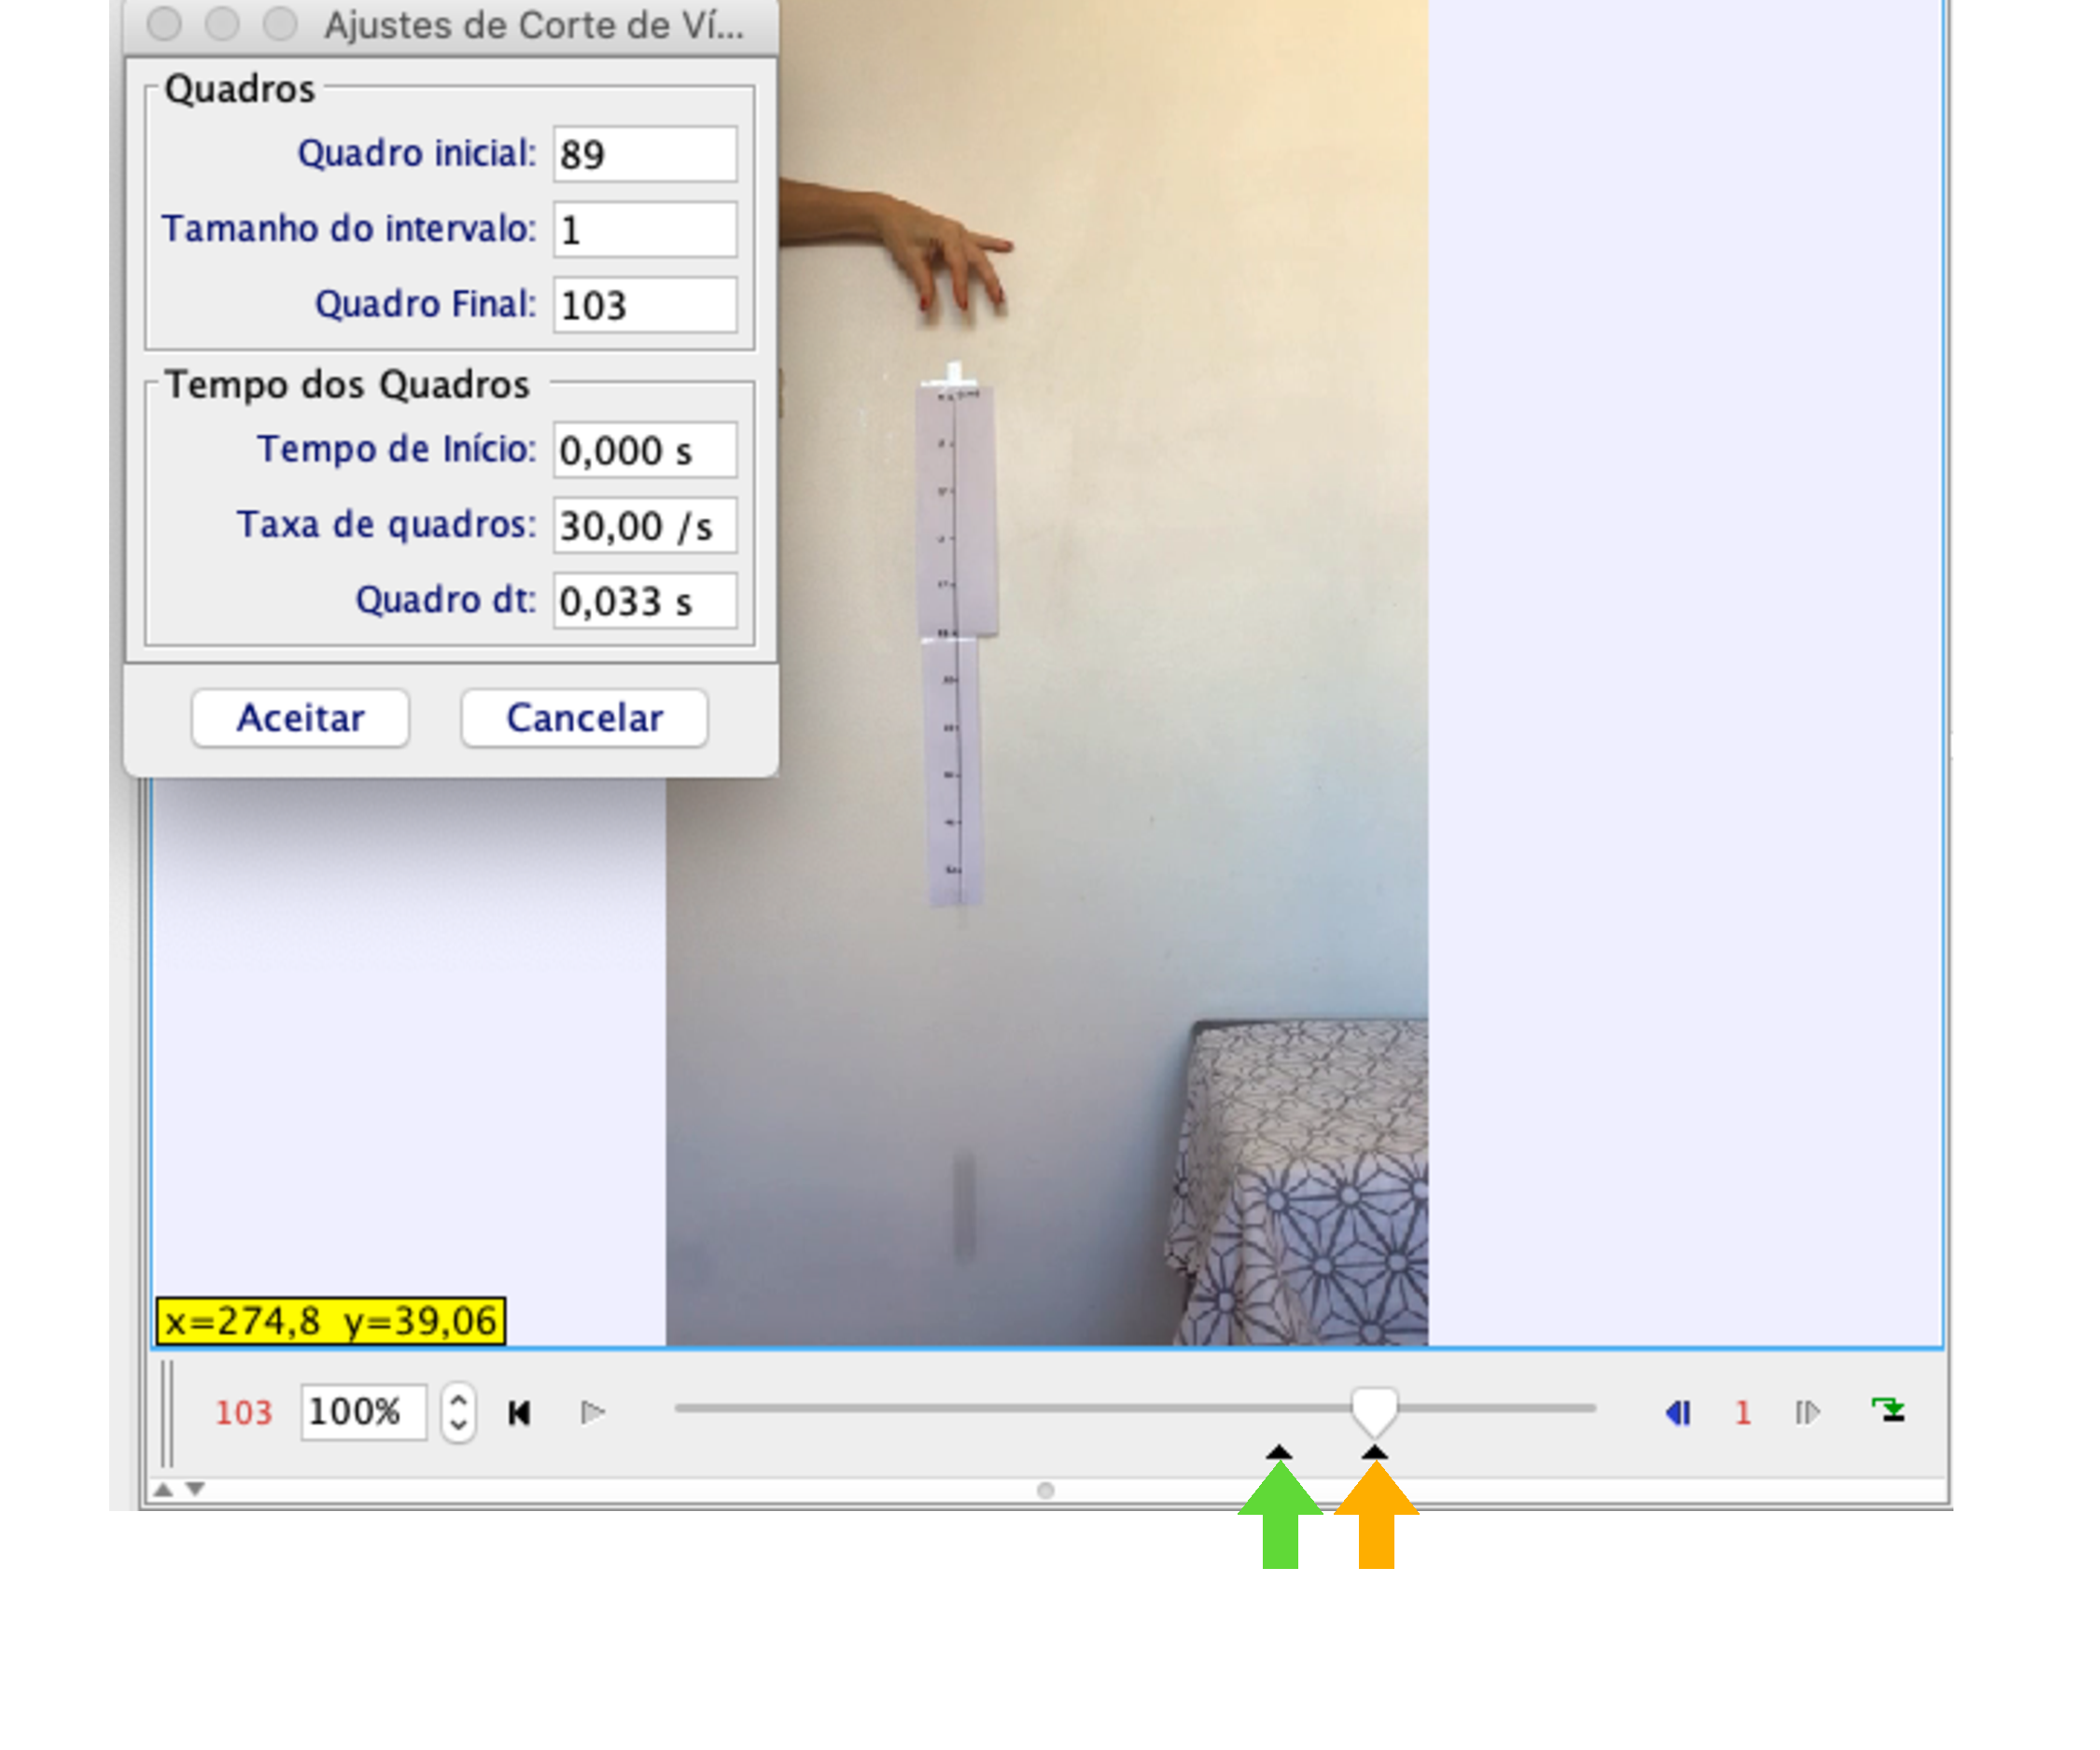
\includegraphics[width=\linewidth]{Figuras_exp3/fig4AppB.pdf}
\caption{\label{fig4AppB} Movimentando os ícones pretos indicados pelas setas verde e laranja escolhemos os quadros iniciais e finais respectivamente.}
          \end{figure}
      \end{minipage}
  \end{minipage}%

\underline{\bf Passo 4:} {\bf Escolha da escala de comprimentos}\\
\vskip -0.5cm

Faça ``click'' no ícone indicado pela seta preta  na Figura~\ref{fig5AppB} e escolha um novo 
``bastão de medição''. De um ``zoom'' na imagem escolhendo o aumento apropriado no ícone da lupa
de maneira de ver claramente a região da régua na imagem do quadro inicial.  
Mantendo apertada a tecla "shift" do computador selecione os pontos iniciais e finais sobre a régua
como indicado na Figura~\ref{fig6AppB}. Não esqueça de colocar na janela indicada nessa figura o valor real do comprimento do ``bastão de medição'' escolhido em metros.
  \begin{minipage}{\linewidth}
 \centering
      \begin{minipage}{0.35\linewidth}
          \begin{figure}[H]
              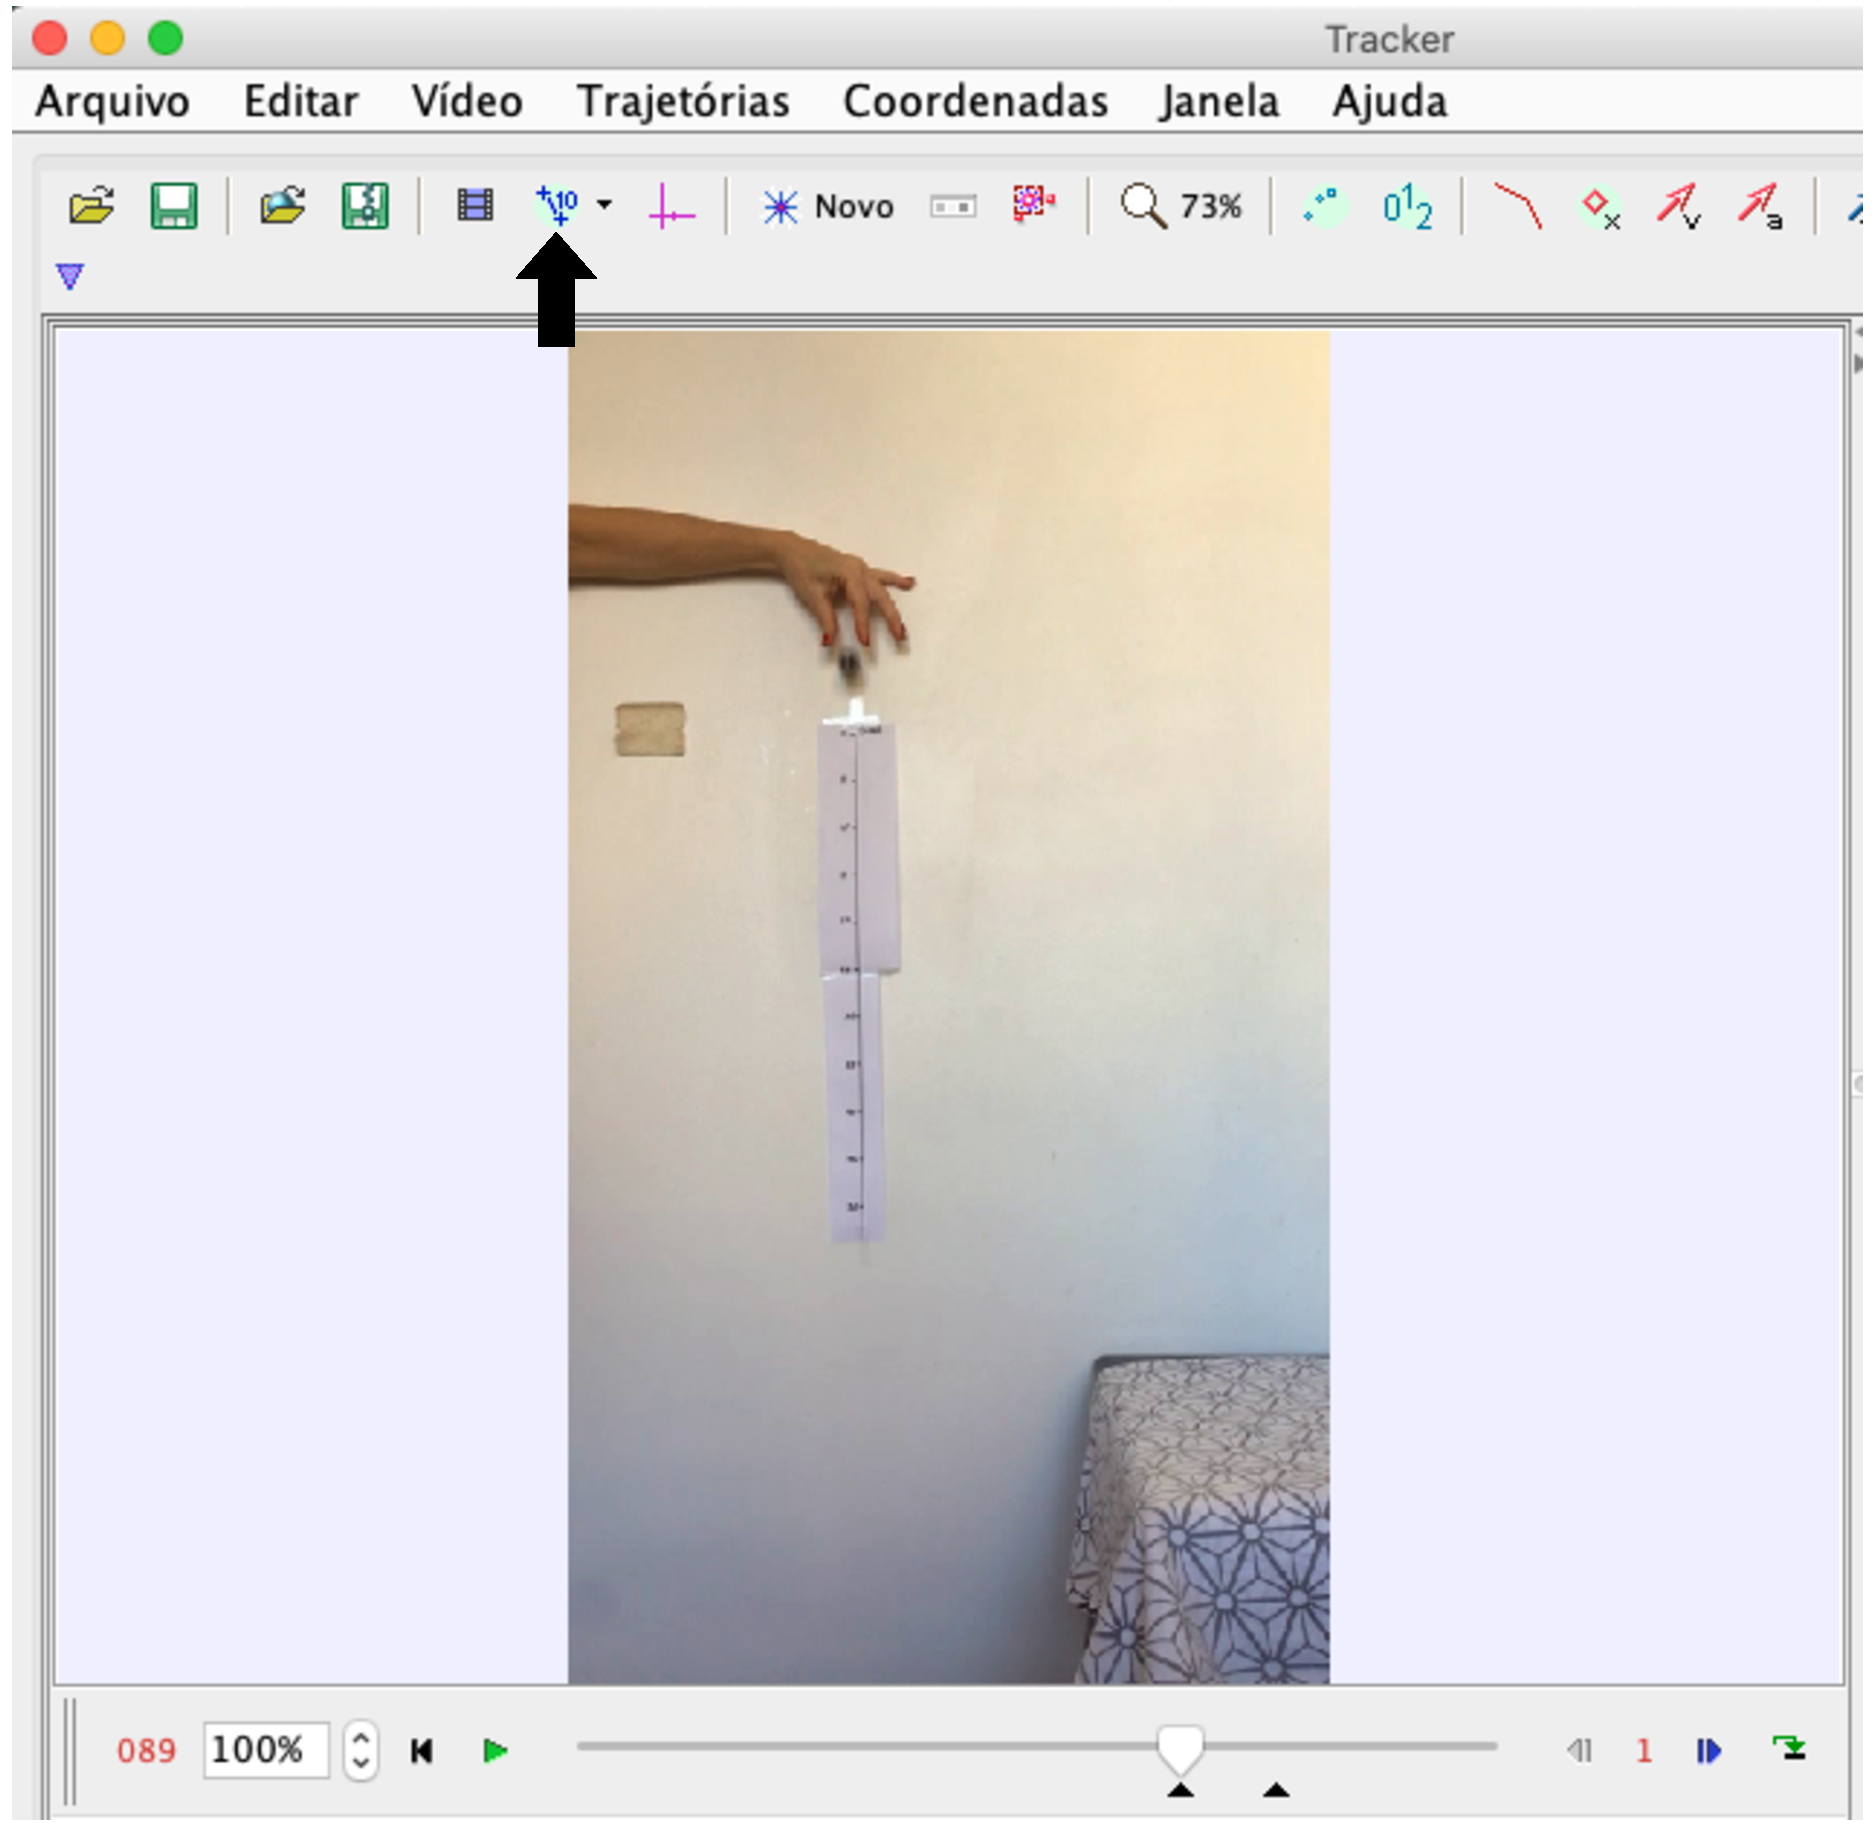
\includegraphics[width=\linewidth]{Figuras_exp3/fig5AppB.pdf}
\caption{\label{fig5AppB} Fazendo ``click no ícone indicado pela seta preta você pode escolher um ``bastão de medição'' que definirá a escala.}
          \end{figure}
      \end{minipage}
      \hspace{0.05\linewidth}
      \begin{minipage}{0.38\linewidth}
          \begin{figure}[H]
              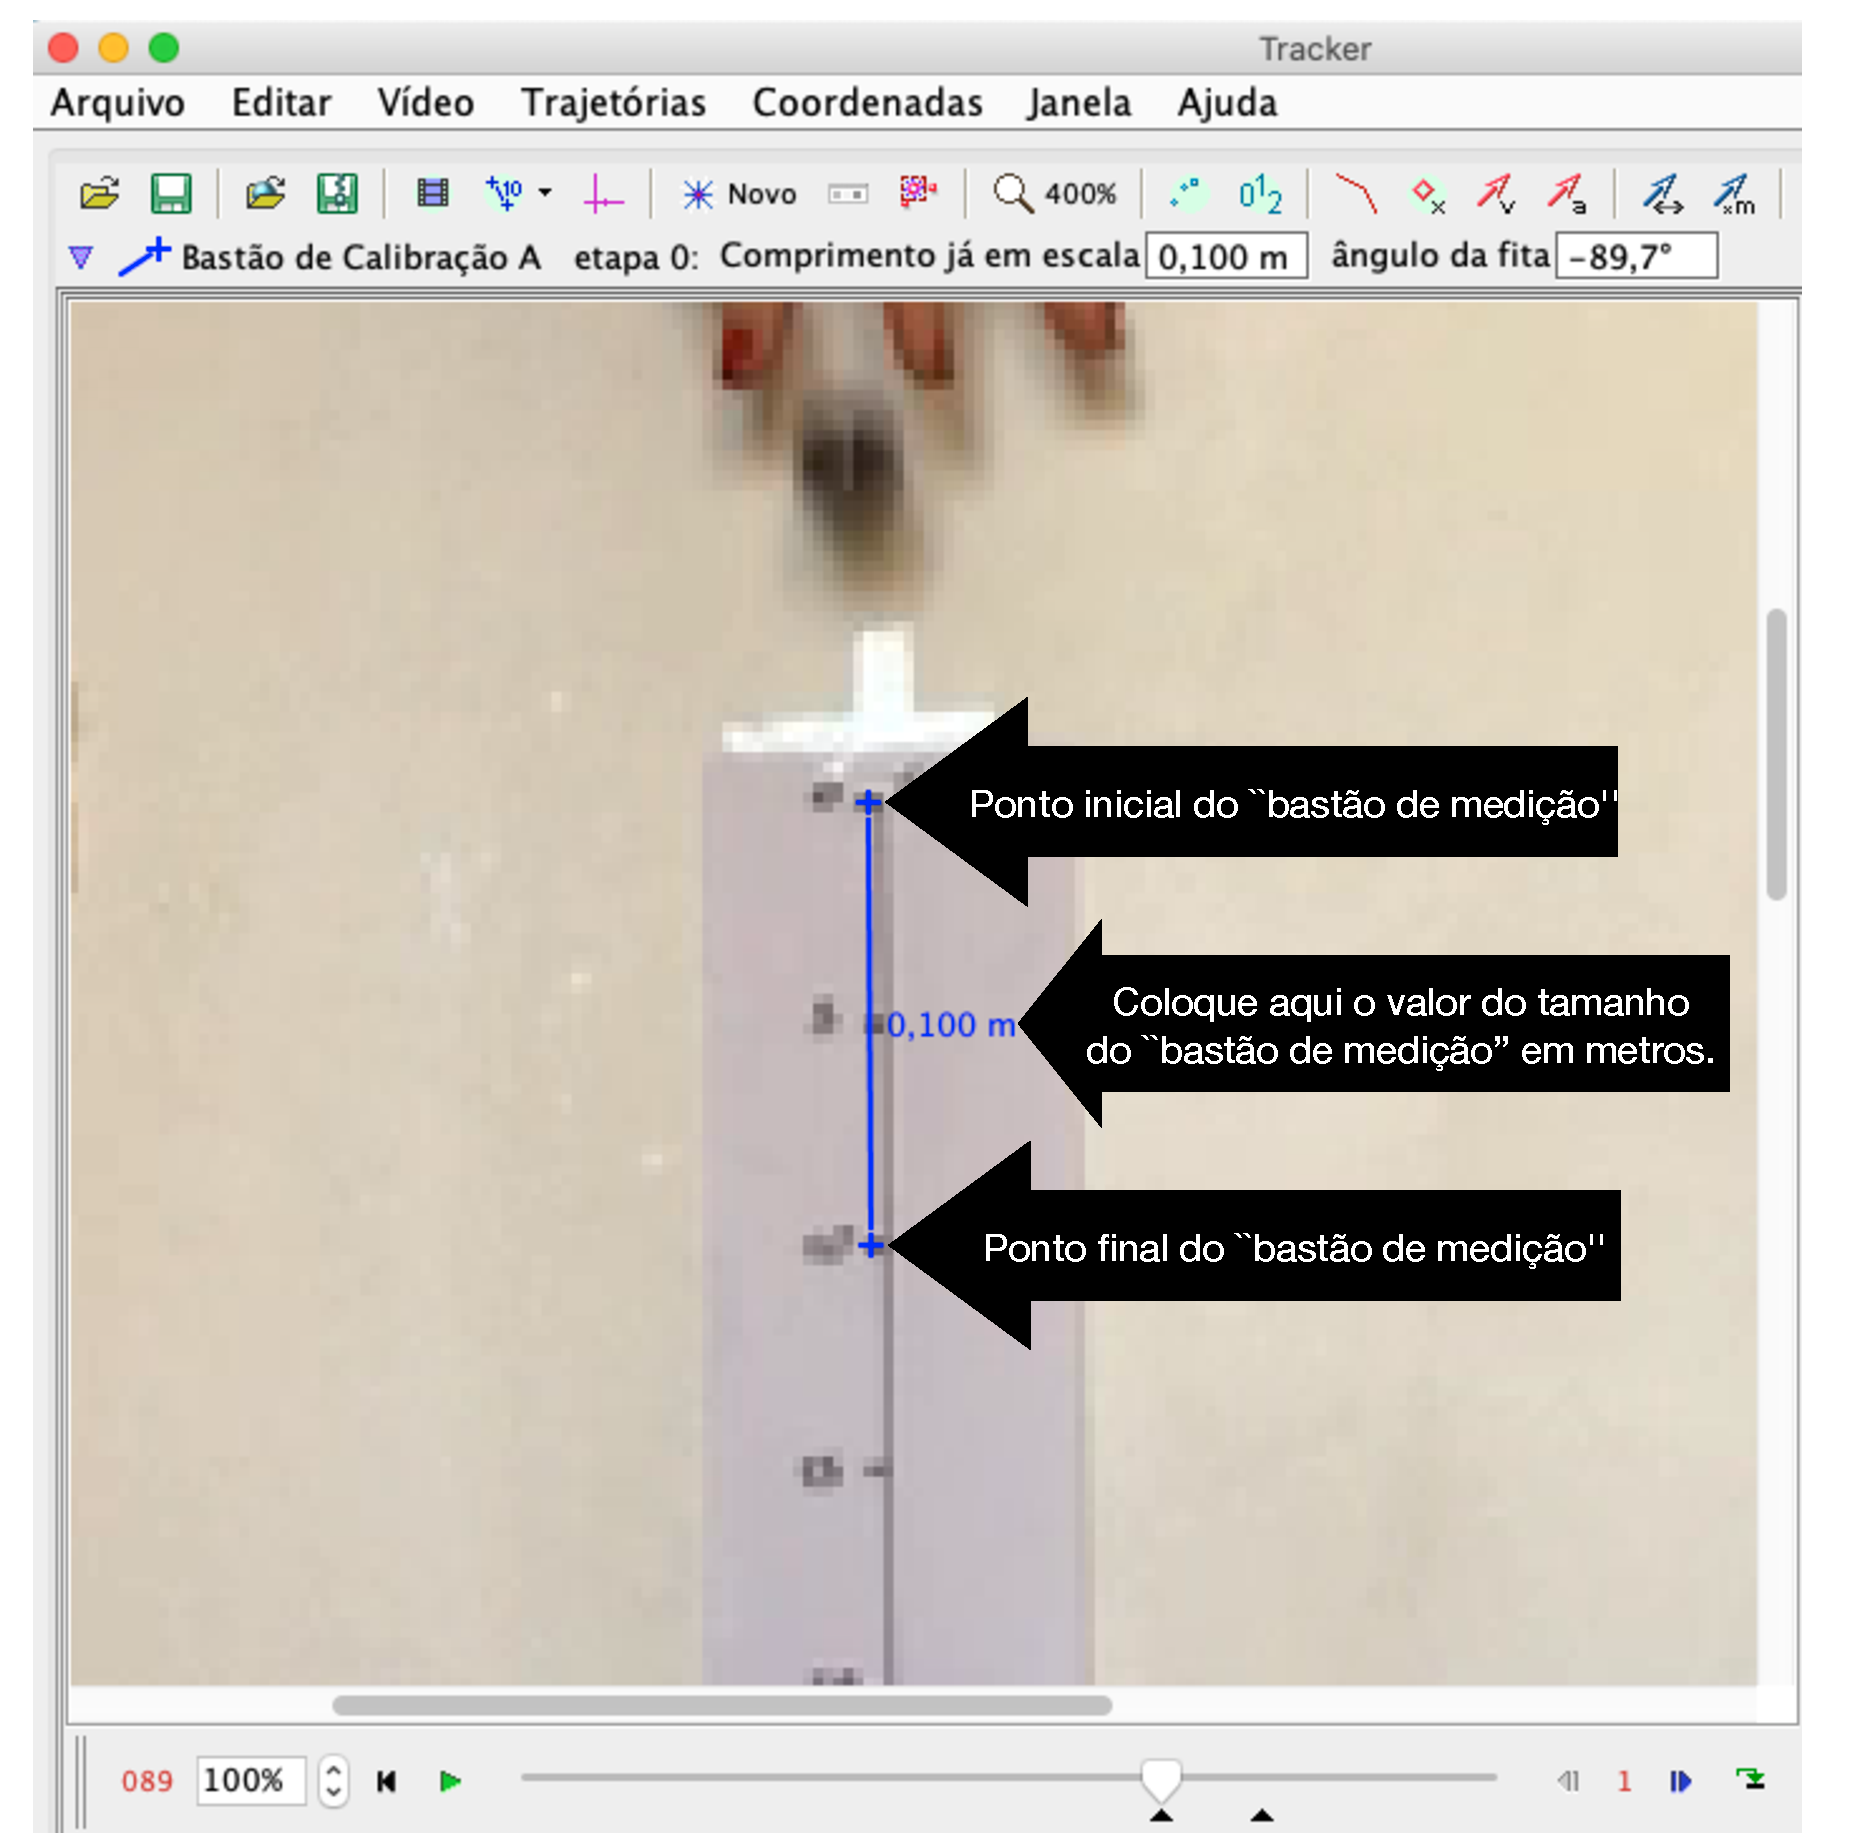
\includegraphics[width=\linewidth]{Figuras_exp3/fig6AppB.pdf}
\caption{\label{fig6AppB} Determinação do ''bastão de medição'' que estabelece a escala de comprimentos.}
          \end{figure}
      \end{minipage}
  \end{minipage}%


\underline{\bf Passo 5:} {\bf Escolha do sistema de coordenadas}\\
\vskip -0.5cm

Para escolher um sistema de eixos coordenados faça ``click'' no ícone indicado pela seta preta na Figura \ref{fig7AppB}. Dessa forma aparecerá o sistema de eixos cor de rosa da figura. Você pode deslocar 
a origem de coordenadas do sistema de eixos fazendo ``click'' com o botão esquerdo do mouse do computador e arrastando a origem para o local que você desejar. Também é possível inclinar o sistema de eixos se for necessário (nesta experiência não será necessário) fazendo ``click'' com o botão esquerdo do mouse do computador em qualquer eixo e arrastando esse eixo para obter a inclinação desejada.

\underline{\bf Passo 6:} {\bf Escolha da janela de controle da massa cuja trajetória
será determinada}\\
\vskip -0.5cm

Fazendo ``click'' no ícone marcado pela seta preta na Figura~\ref{fig8AppB} se abrirá a janela de controle 
 da massa (indicada pela seta vermelha  na Figura~\ref{fig8AppB}, cuja trajetória será determinada (neste caso a bolinha da figura). Fazendo ``click'' na seta verde você poderá escolher qual gráfico 
 quer visualizar uma vez escolhidos os pontos da trajetória cuja forma será ensinada no próximo passo deste tutorial.
Também fazendo ``click'' na aba ``Dados'' assinalada pela seta azul na  Figura~\ref{fig8AppB} se abrirá a janela onde você poderá selecionar (seta rosa na figura) as colunas que apareceram na janela de tabelas (indicada também na figura).
  \begin{minipage}{\linewidth}
      \centering
      \begin{minipage}{0.35\linewidth}
          \begin{figure}[H]
              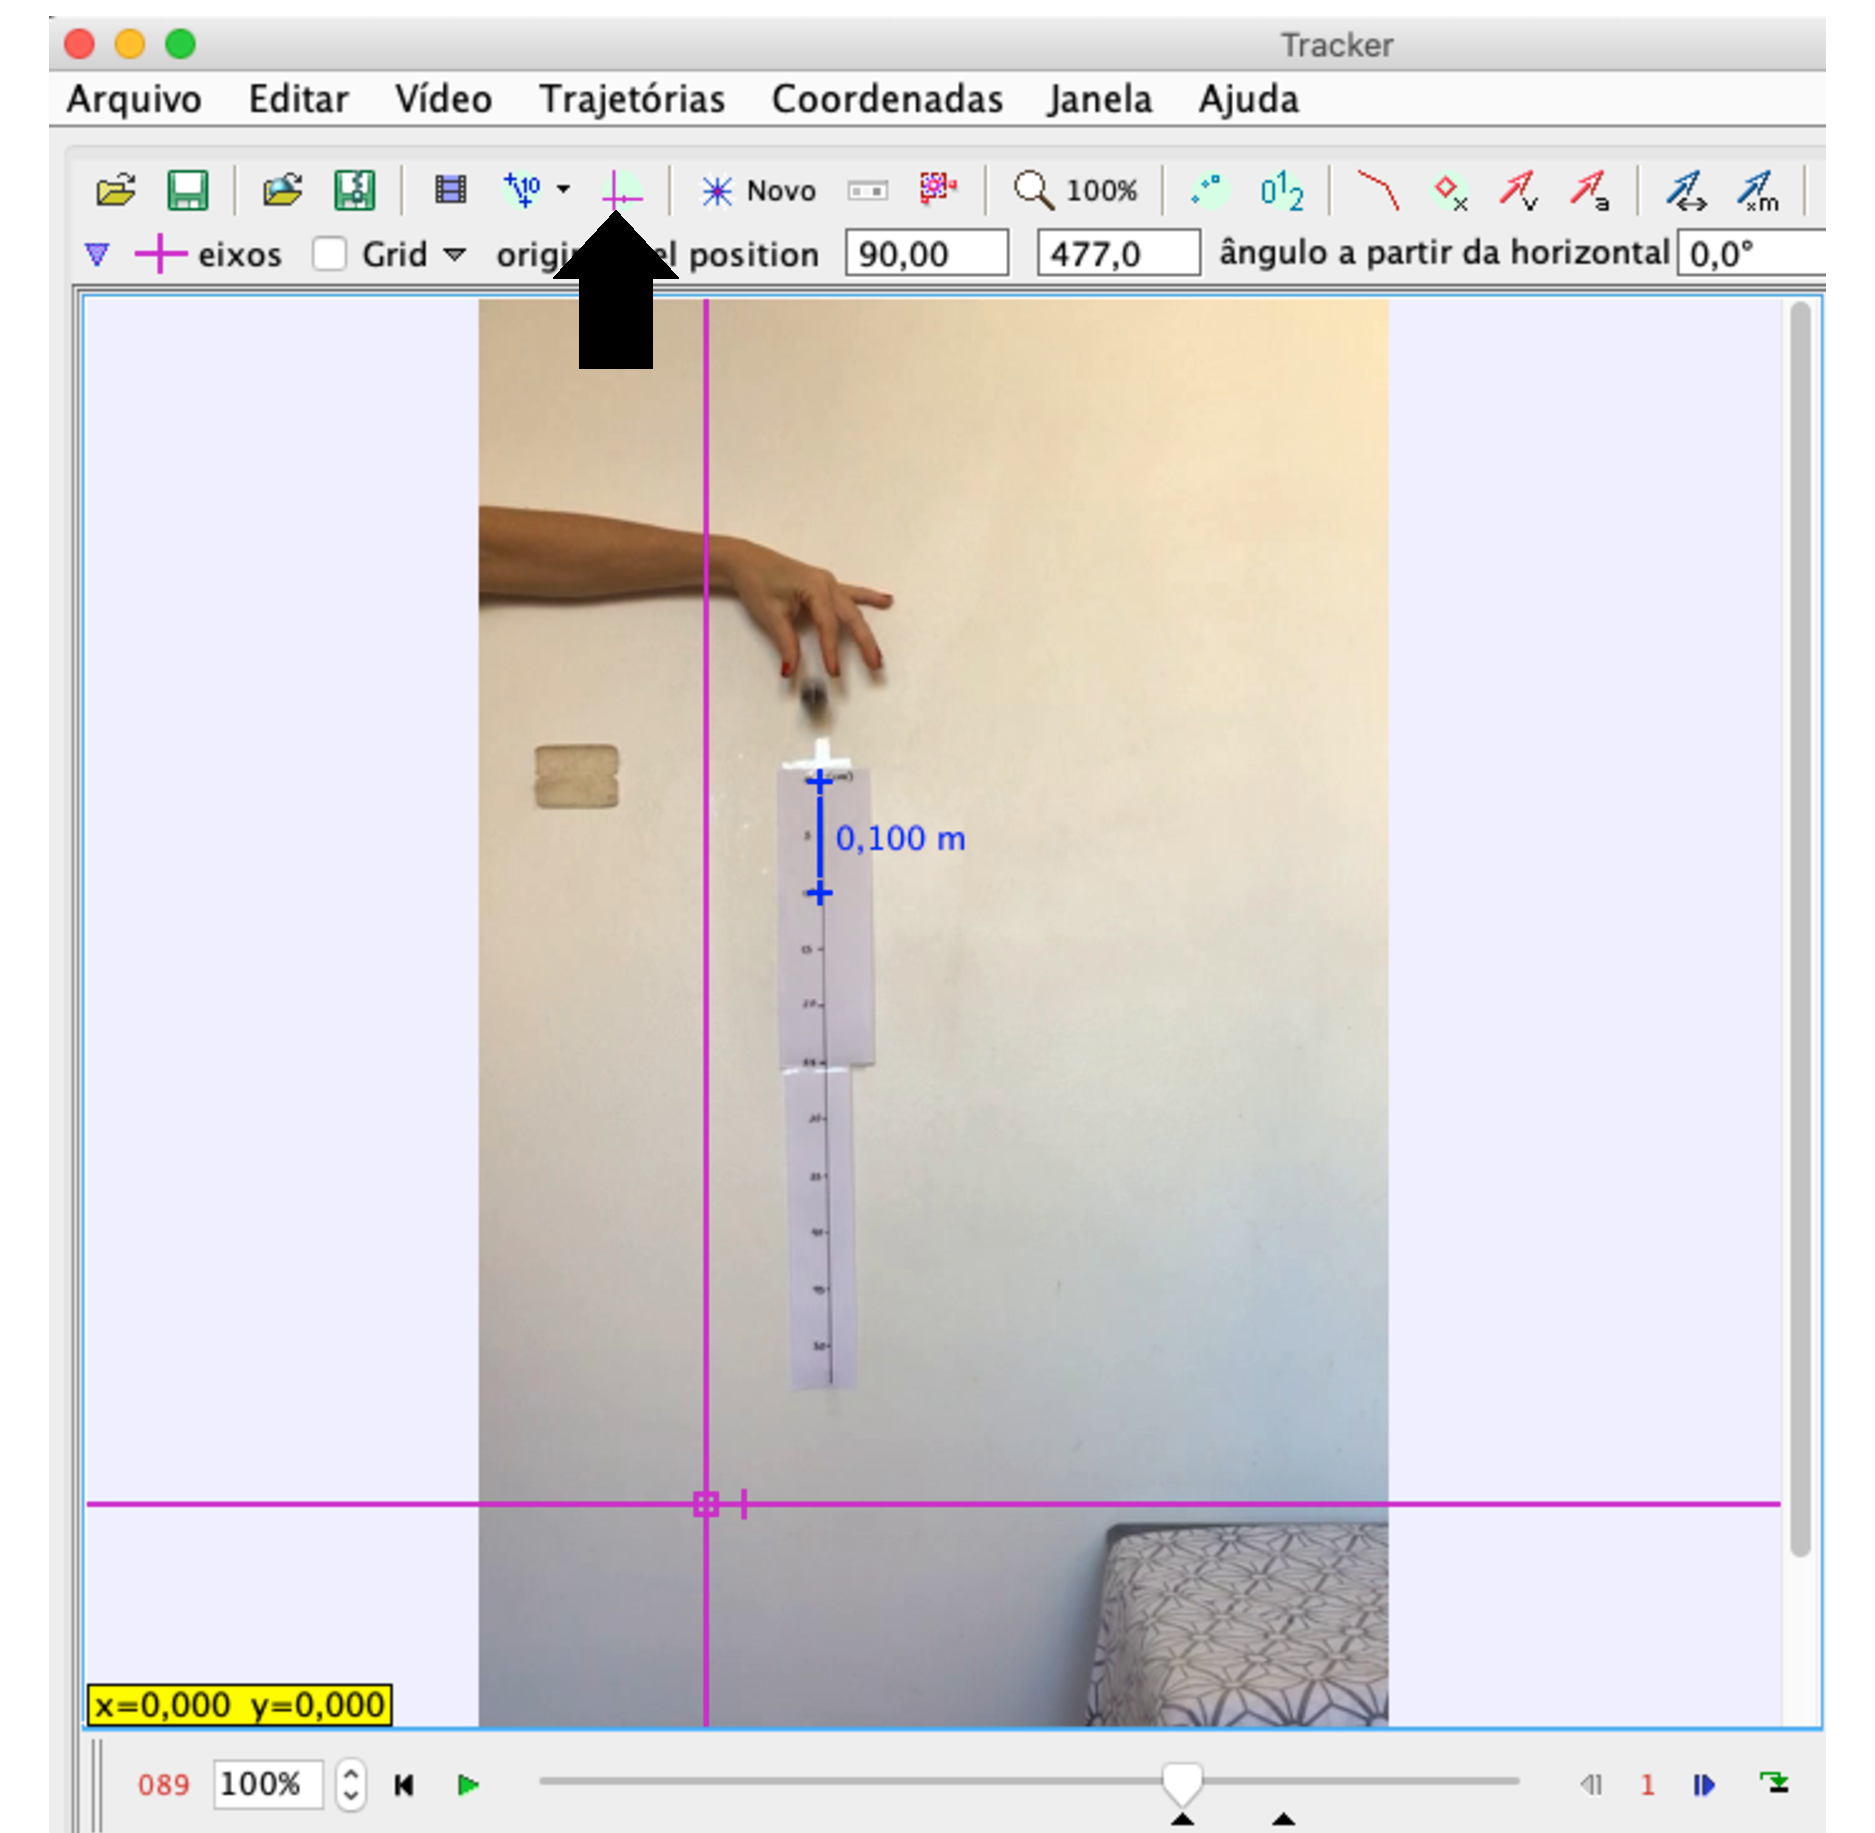
\includegraphics[width=\linewidth]{Figuras_exp3/fig7AppB.pdf}
\caption{\label{fig7AppB} Para criar um sistema de coordenadas (eixos de cor rosa na Figura) faça ``click'' no ícone indicado pela seta preta. Logo posicione a origem de coordenadas, como mostrado na figura, arrastando com o mouse do computador o quadrado rosa no sistema de eixos.}
          \end{figure}
      \end{minipage}
      \hspace{0.05\linewidth}
      \begin{minipage}{0.37\linewidth}
          \begin{figure}[H]
              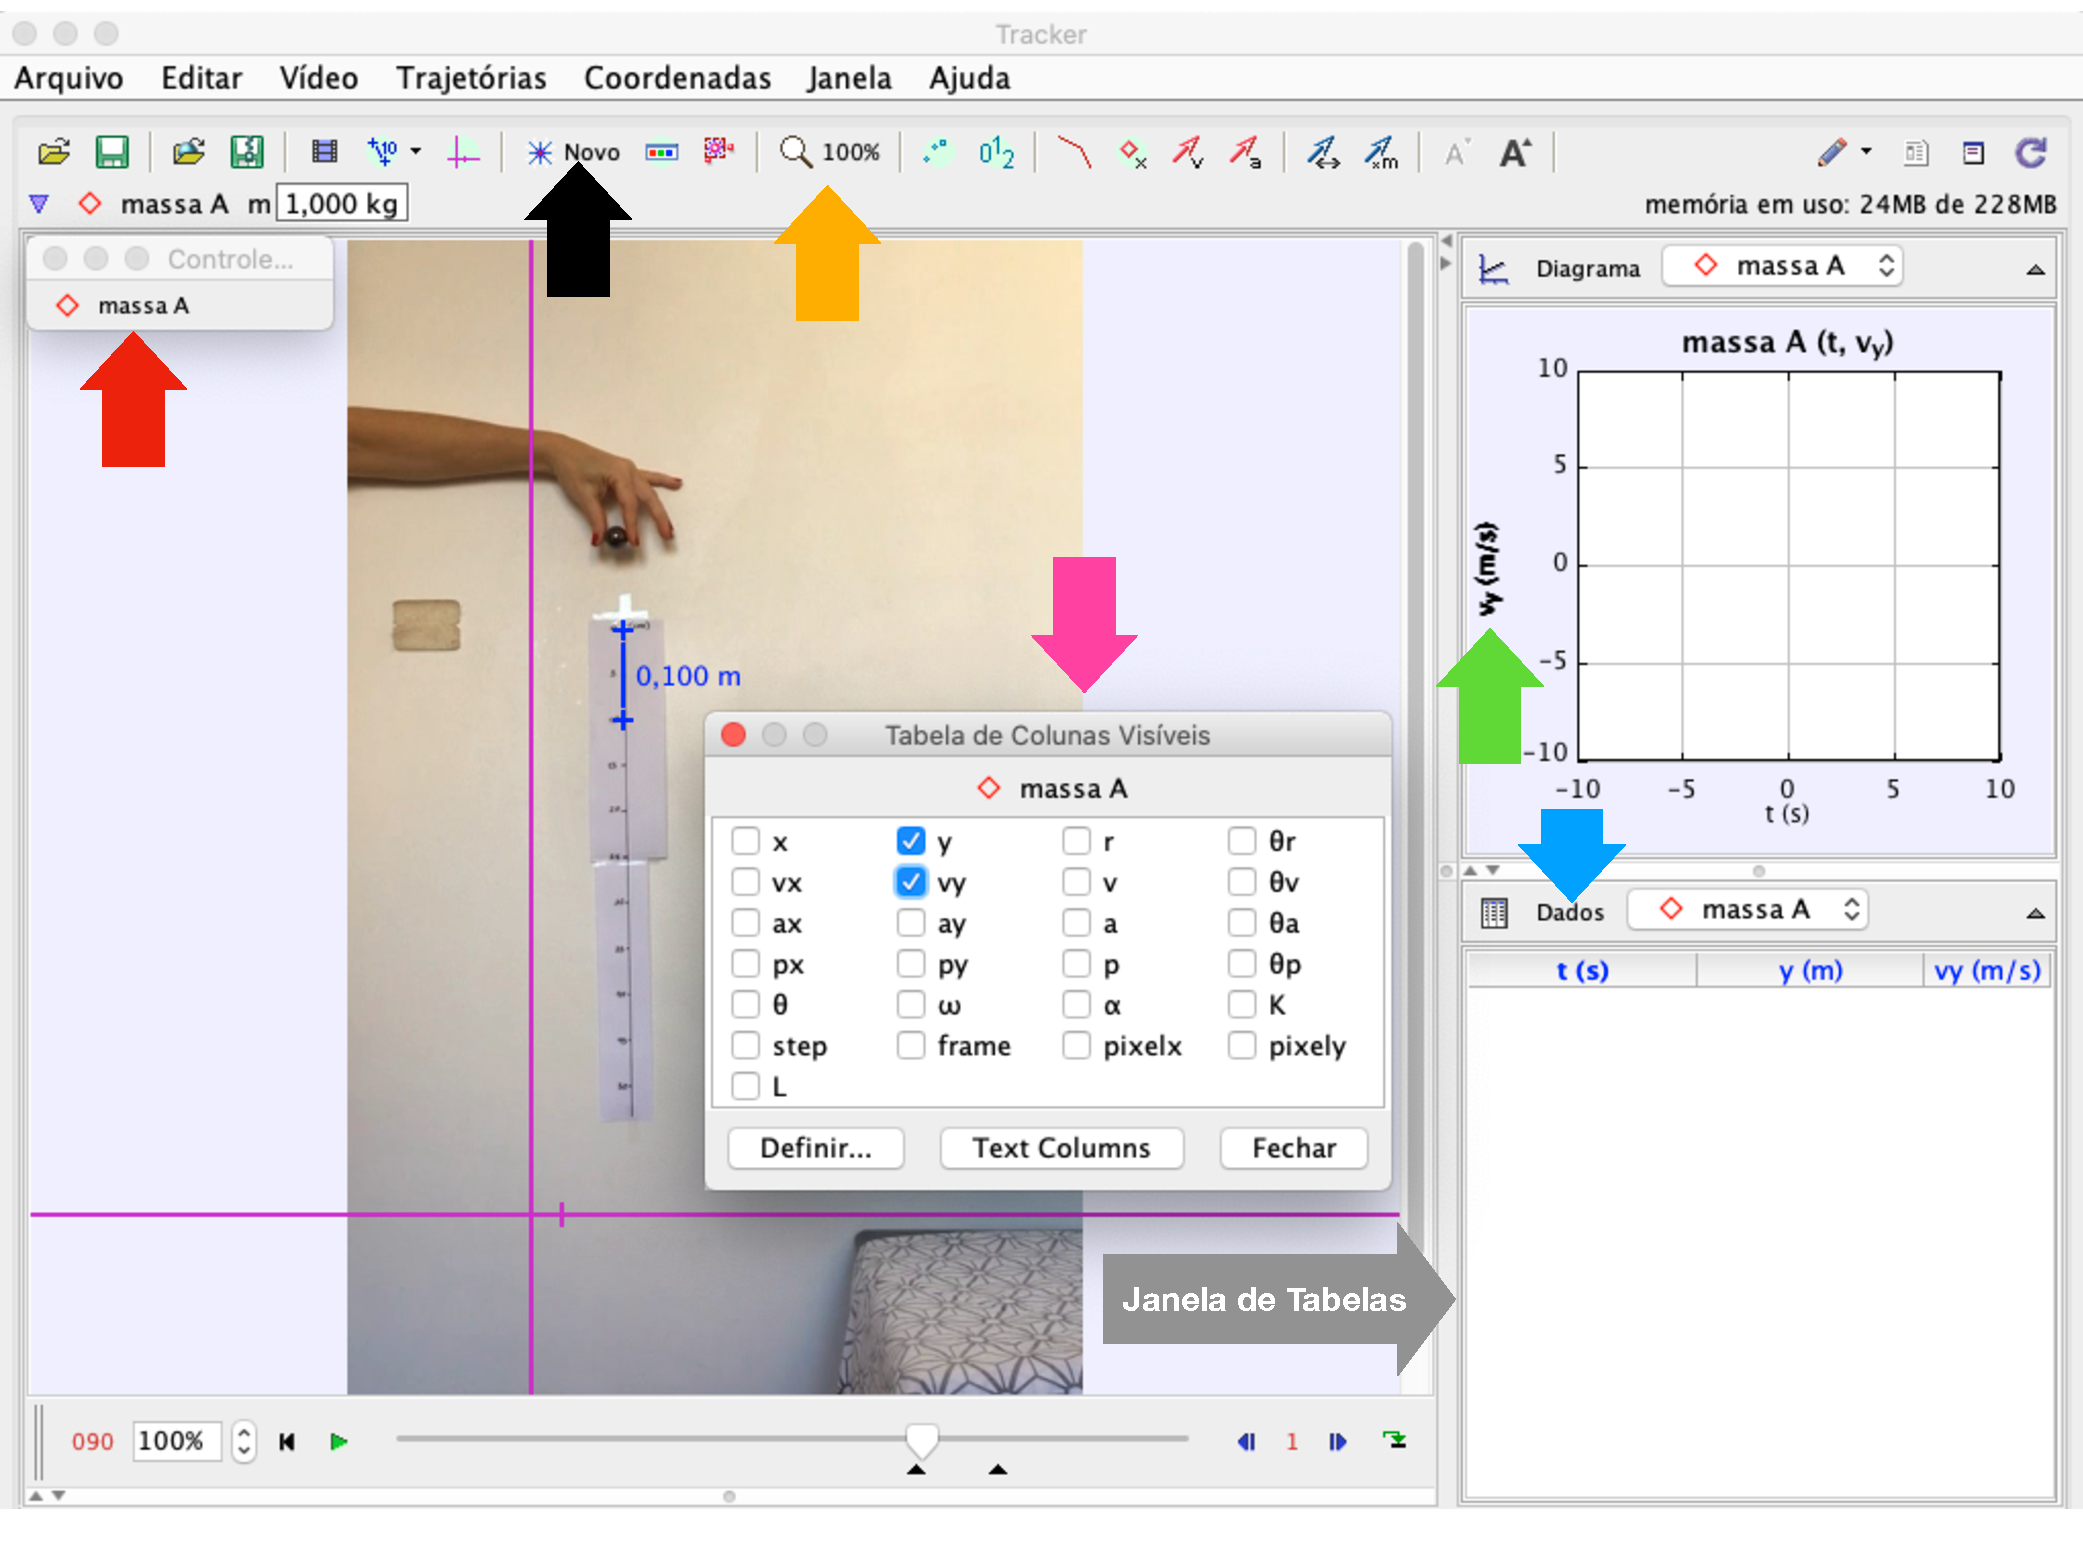
\includegraphics[width=\linewidth]{Figuras_exp3/fig8AppB.pdf}
\caption{\label{fig8AppB} Fazendo ``click'' no ícone indicado pela seta preta abre-se a janela indicada pela seta vermelha. Fazendo ``click'' no ícone indicado pela seta verde se escolhe o gráfico que quer ser visualizado 
após determinar os pontos da trajetória. Fazendo ``click'' na aba ``Dados'', indicada pela seta azul, 
abre-se a janela indicada pela seta rosa onde podem ser escolhidas as colunas das tabelas de dados que apareceram na janela de tabelas. Se precisar fazer um zoom na imagem pode usar a aba indicada pela seta laranja.}
          \end{figure}
      \end{minipage}
  \end{minipage}%
  
  
  
\underline{\bf Passo 7:} {\bf Determinação dos pontos da trajetória de uma partícula}\\


Para determinar os pontos da trajetória em forma manual você precisará manter 
apertada a tecla ``shift'' do computador durante todo o processo de medida . Ao apertar a tecla ``shift'' você entra no modo aquisição de dados e verá que o cursor virá um quadrado com um ``x'' no meio.
Ao fazer ``click'' no ponto que você quer traçar a trajetória (no nosso caso será o centro da bolinha)
pela primeira vez se marca um ponto da trajetória e a imagem pula automaticamente para o próximo quadro e ali você pode marcar o centro da bolinha novamente. Repita esse processo até marcar todos os pontos da trajetória contidos nas imagens entre os quadros iniciais e finais determinadas no passo 3 deste tutorial. À medida que você vai marcando os pontos da trajetória as colunas nas tabelas de dados (ver Figura~\ref{fig8AppB}) vão sendo preenchidas em forma automática.
\begin{figure}[h!]
      \centering
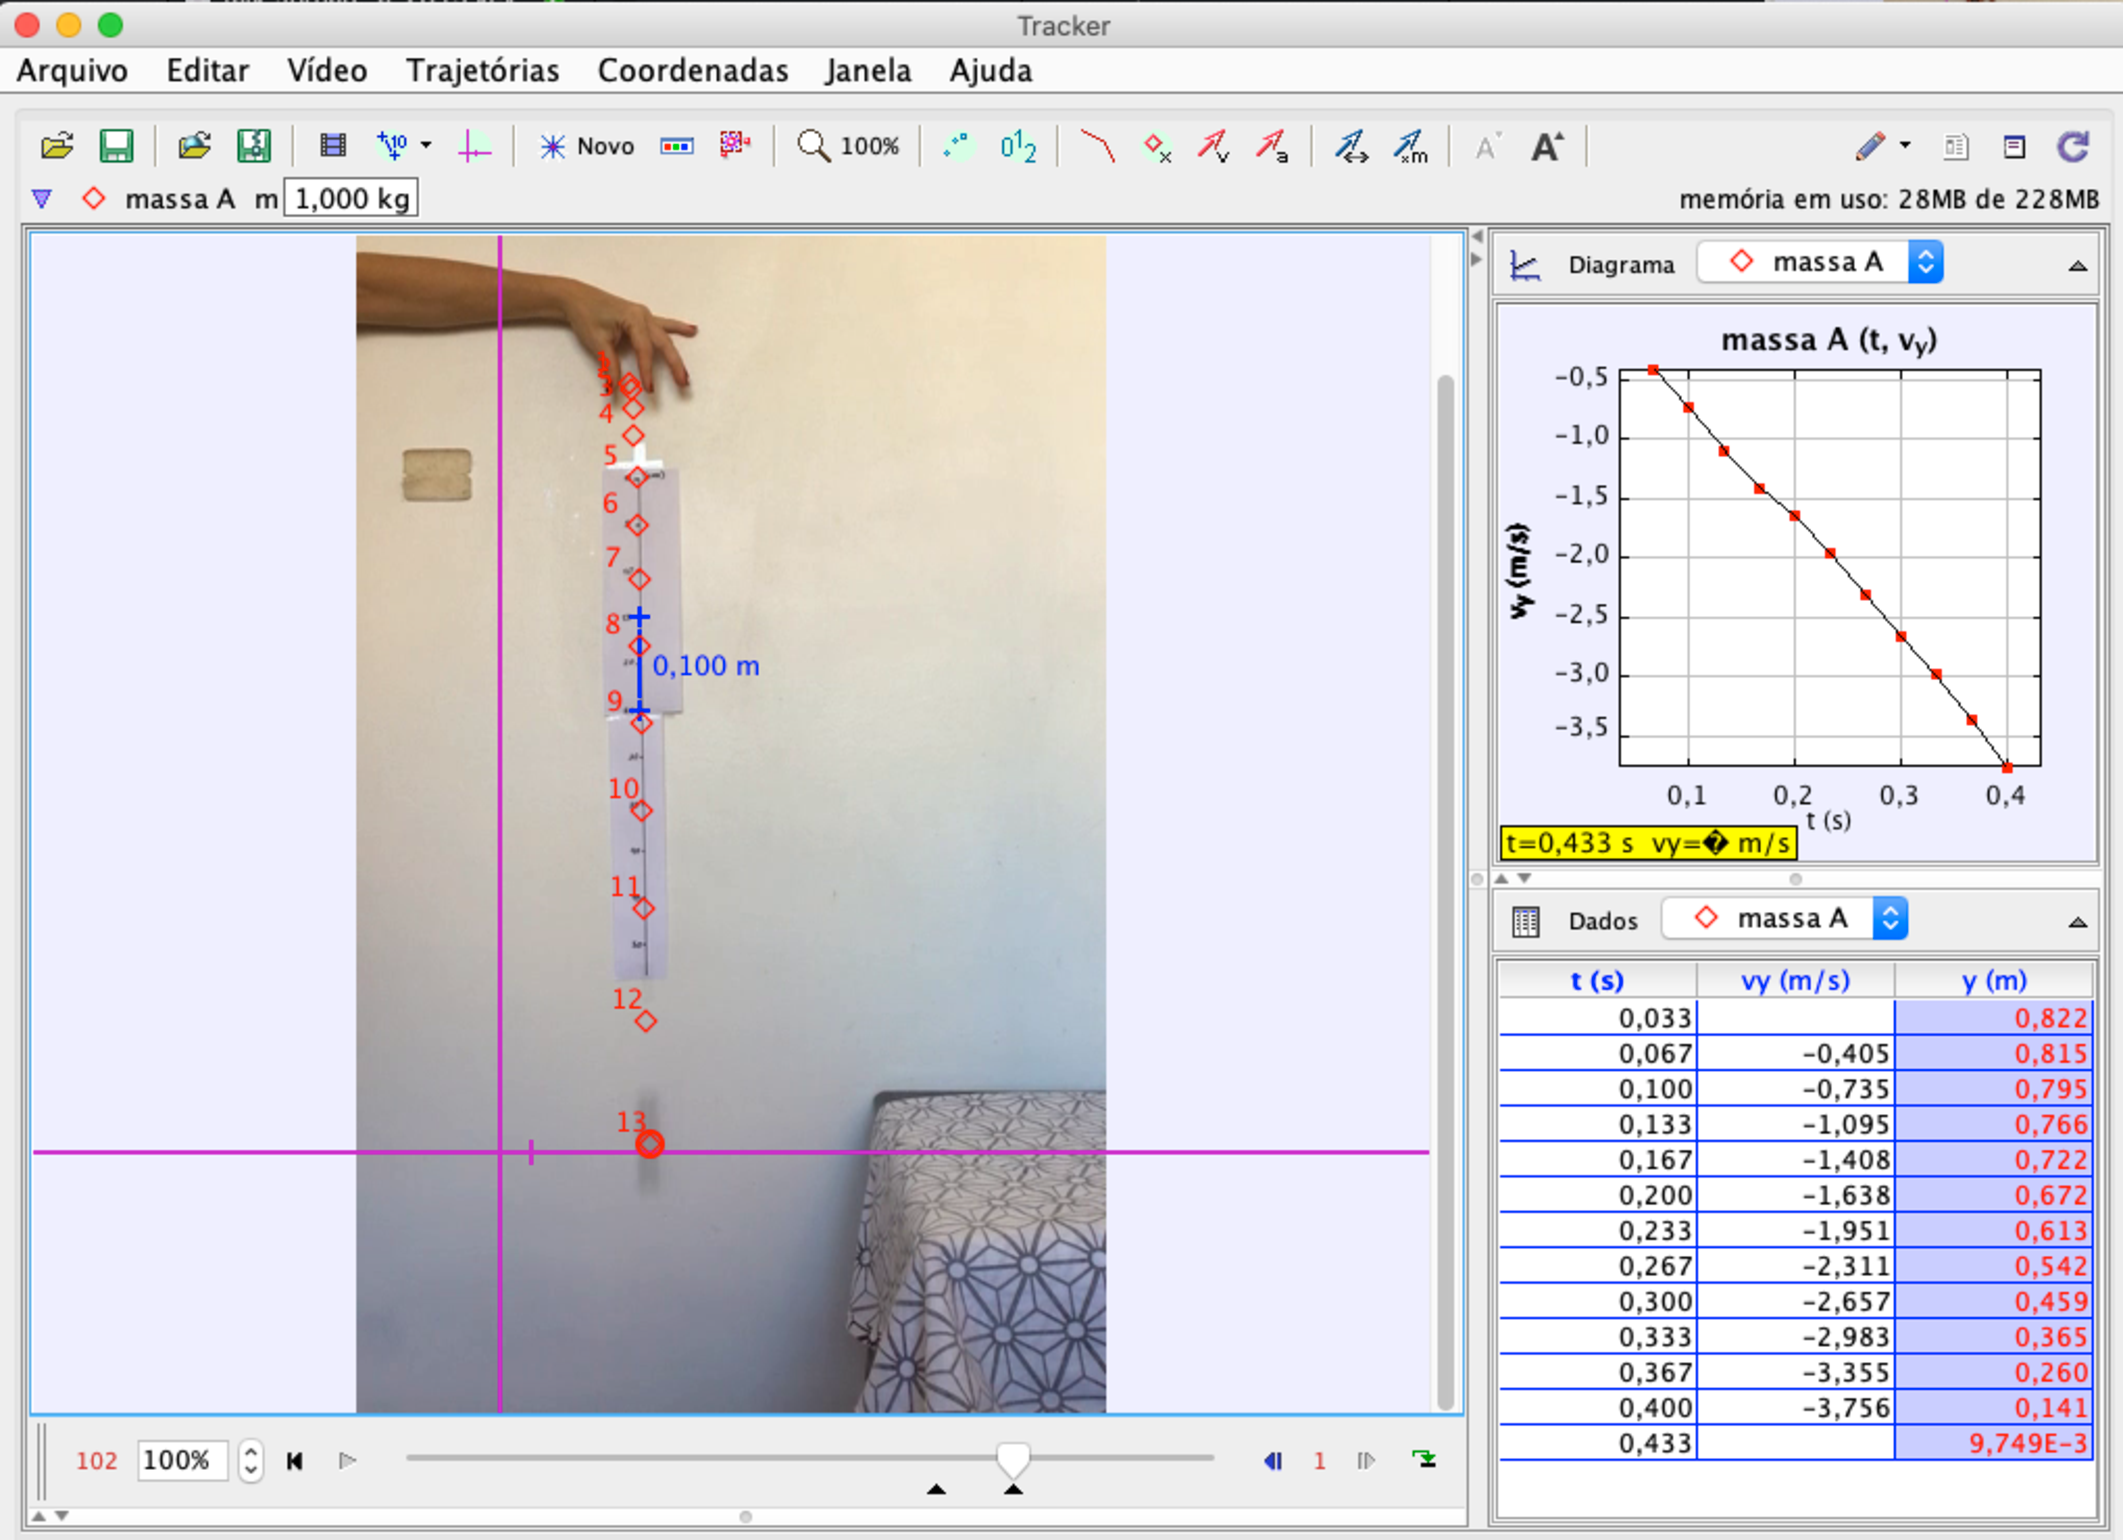
\includegraphics[width=9cm]{Figuras_exp3/fig9AppB.pdf}
\caption{\label{fig9AppB} Pontos da trajetória marcados e dados coletados nas colunas da janela de tabela.}
\end{figure}
No processo de medida é importante se auxiliar da ferramenta zoom, indicada pela seta laranja na 
Figura~\ref{fig8AppB}, para ter uma melhor imagem da bolinha e poder determinar com melhor precisão o seu centro. Uma vez escolhido um zoom (por exemplo $400\%$) para enquadrar a imagem 
da bolinha arraste a imagem com o mouse. Na Figura~\ref{fig9AppB} é mostrado 
o final do processo de medida. Fazendo ``double click'', com o botão esquerdo do mouse, no cabeçalho de uma coluna, na janela de tabela, você seleciona a janela e os valores ficaram da cor rosa como estão os valores da coordenada ``y'' na Figura~\ref{fig9AppB}. Uma vez selecionada a 
coluna, fazendo ``click'' com o botão direito do mouse você abrira uma janela com varias opções.
Na aba ``Números'' você poderá escolher o formato (sem com vírgula ou ponto para separar os decimais). Uma vez escolhido o formato você poderá copiar os dados selecionados para serem transferidos, por exemplo, para uma planilha tipo Excel. 
 
\chapter{Tutorial básico de uso do aplicativo VidAnalysis}
\label{sec:vidanalysis}
\vspace{-0.7cm}

 
VidAnalysis é um aplicativo para análise física de movimentos em vídeos muito fáceis de usar.
O aplicativo é compatível com Android e pode ser baixado gratuitamente em \href{https://play.google.com/store/apps/details?id=com.vidanalysis.free}{\textcolor {blue}
{https://play.google.com/store/apps/details?id=com.vidanalysis.freey}}, ou simplesmente pesquise no Google Play com o nome VidAnalysis free. O aplicativo possui apenas uma versão em inglês, mas devido à simplicidade de seu uso, ele não representa nenhum problema.

Para realizar a coleta de dados das posições do objeto gravado no vídeo, siga as etapas abaixo:

\underline{\bf Passo 1:} {\bf Abertura do vídeo a ser analisado}\\


Primeiro, temos que gravar um vídeo ou importar um existente. Se você decidir importar um vídeo, ``click'' no sinal de adição mostrado com uma seta preta na Figura~\ref{apendice1c}. Como o aplicativo VidAnalysis suporta apenas formatos de vídeo com extensão ``mp4'' é recomendável gravar  diretamente dentro do aplicativo, escolhendo a opção marcada pela seta vermelha na Figura~\ref{apendice1c}.
Ao capturar vídeos para análise, é importante que a câmera esteja fixa, que o movimento esteja dentro do plano da câmera, e que no vídeo gravado apareça alguma referencia de 
um comprimento conhecido, por exemplo de uma régua. 

\begin{figure}[h!]
\centering
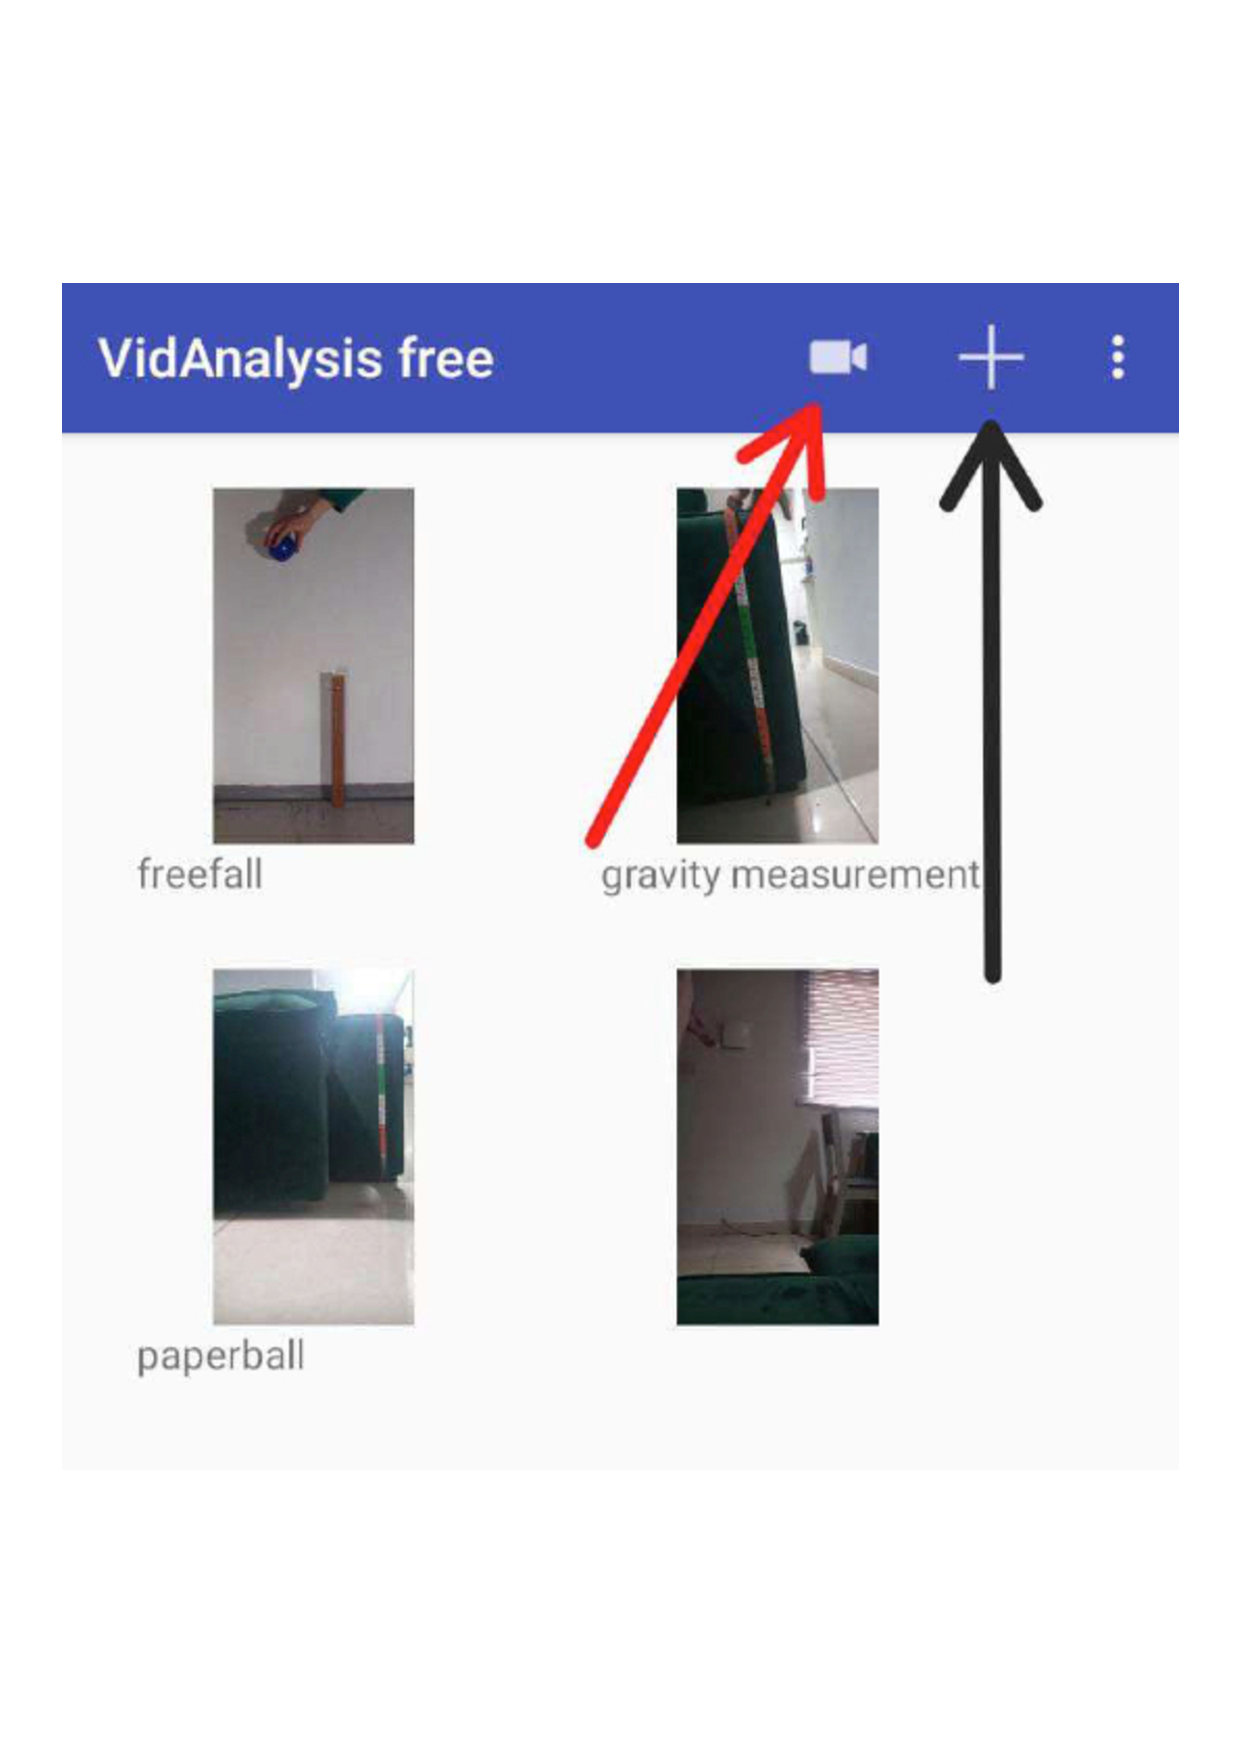
\includegraphics[width=8cm]{Figuras_exp3/imagenapendicec1.pdf}
\caption{\label{apendice1c} Menu do aplicativo VidAnalysis.}
\end{figure}

\vskip 0.5cm
\underline{\bf Passo 2:} {\bf Calibração}\\


Para começar a análise do movimento do objeto primeiramente  
selecionamos o vídeo no reprodutor e será aberta a primeira imagem dele como se mostra na Figura \ref{apendice2c}. É importante avançar o vídeo nessa tela, para começar a coleta de dados da trajetória do objeto diretamente no momento em que o movimento  começa, para isso fazemos ``click'' no botão mostrado pela seta verde na Figura~\ref{apendice2c} até avançarmos ao quadro do vídeo que interessa. Fazendo ``click'' nos três pontos indicado pela seta azul na Figura~\ref{apendice2c}, conseguimos ocultar o menu em preto, para uma melhor visualização do vídeo.

\begin{figure}[h!]
\centering
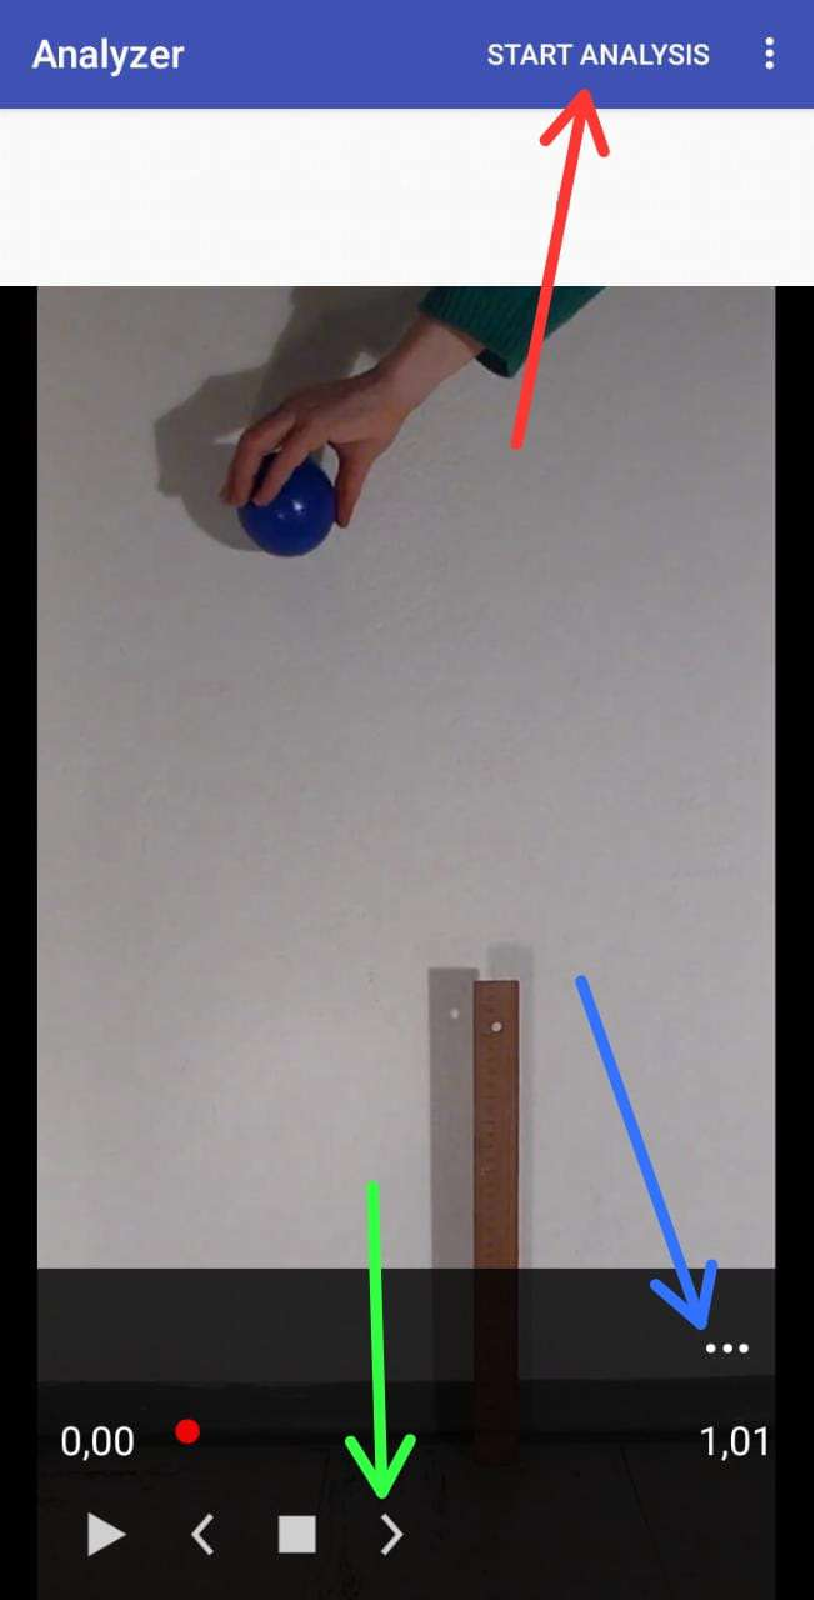
\includegraphics[width=8cm]{Figuras_exp3/imagenapendicec2.pdf}
\caption{\label{apendice2c} Reprodutor de video do aplicativo VidAnalysis.}
\end{figure}

Antes da coleta de dados deve primeiro calibrar qual é a escala de comprimentos que será usada pelo aplicativo. Para isso, fazemos ``click'' na aba ``start analysis''  no canto superior direito na Figura \ref{apendice2c}. Agora temos que marcar o comprimento conhecido.
 Ao fazer ``click no ponto inicial do comprimento conhecido, na tela esse ponto será marcado com uma cruz azul. Em seguida, deve fazer “click“ novamente no ponto final do comprimento conhecido e outra cruz azul indicará esse ponto. Após finalizar essa segunda marcação abrirá imediatamente uma janela solicitando o tamanho conhecido, como mostramos na Figura~\ref{apendice3c}. A legenda em inglês na janela pergunta ``Qual é o comprimento real disto em metros'' (``How many meters is this in real'' em inglês). É importante saber que a unidade a ser usada pelo aplicativo para comprimentos é sempre metros portanto as velocidades serão em metros por segundo por exemplo.
 
\begin{figure}[h!]
\center
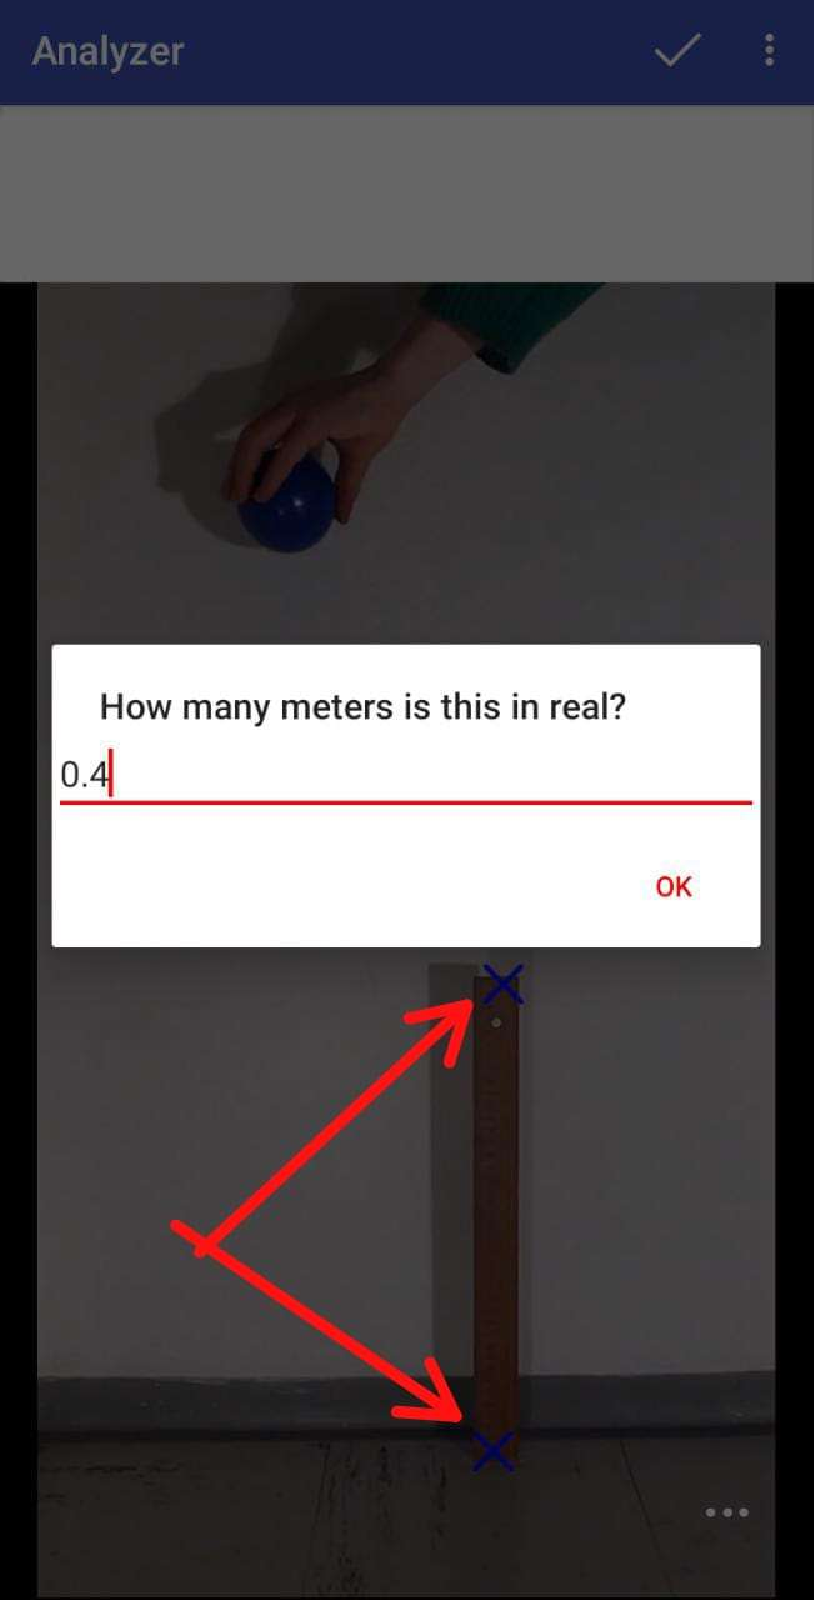
\includegraphics[width=8cm]{Figuras_exp3/imagenapendicec3.pdf}
\caption{\label{apendice3c} Escolha da escala de comprimentos no reprodutor de vídeo do aplicativo VidAnalysis, a ser usado na tomada de dados dos pontos da trajetória do objeto.}

\end{figure}
Após dar ``ok'' na janela da escala aparecerá um sistema de eixos coordenados cuja origem devemos estabelecer (ver Figura  \ref{apendice4c}). Em geral, é uma boa ideia posicionar a origem de coordenadas de tal maneira que as coordenadas da posição do objeto sempre tenham o mesmo sinal ao longo da trajetória.

\begin{figure}[h!]
\centering
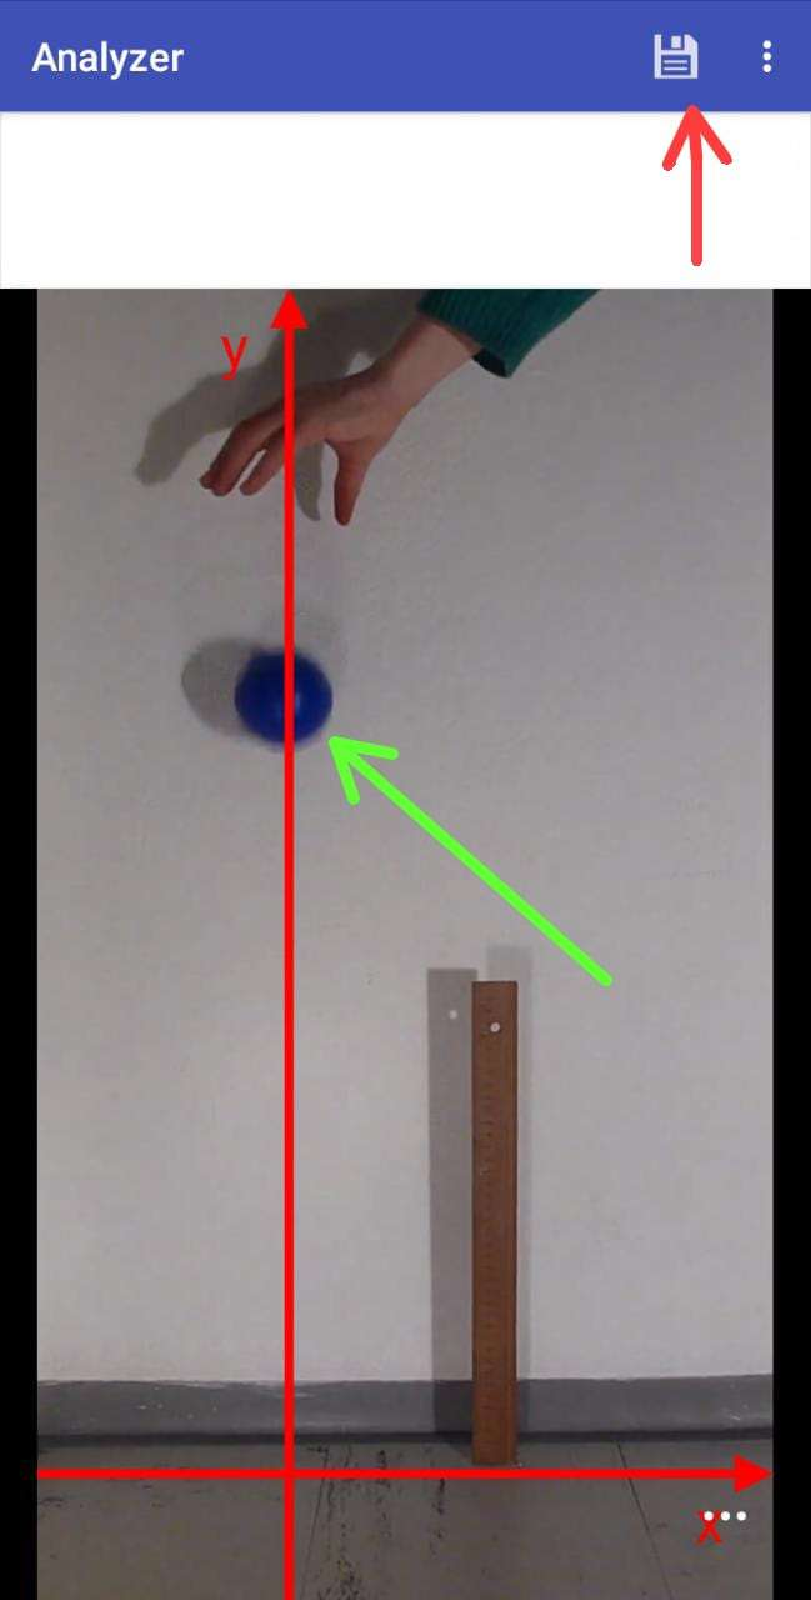
\includegraphics[width=8cm]{Figuras_exp3/imagenapendicec4.pdf}
\caption{\label{apendice4c} Sistema de eixos no reprodutor de vídeo do aplicativo VidAnalysis.}
\end{figure}


\underline{\bf Passo 3:} {\bf Coleta de dados}\\


A coleta de dados começa fazendo um ``click com o dedo no ponto do objeto que queremos seguir a trajetória, por exemplo no meio da bolinha azul na Figura~\ref{apendice4c}. Como as marcações são feitas com o dedo sugerimos que o corpo, cuja trajetória será determinada, seja suficientemente grande.
Depois que o primeiro ``click'' for feito, uma cruz azul aparecerá e o vídeo avançará alguns quadros. O intervalo de tempo transcorrido, medido em segundos, entre um ``click e outro e automaticamente determinado pelo programa. Vamos fazer ``click'' novamente tantas vezes como seja necessário para acompanhar a evolução da posição do objeto entre a posição inicial e final previamente estabelecidas. Leve em conta que para uma bolinha em queda vertical uma distância percorrida de um metro é o mínimo necessário para efetuar a análise, mas também não é necessário acompanhar 
todo o movimento do corpo até o chão.
\par 
Como mostrado na  Figura\ref{fig:reguacomxis},  pode ser que ao longo da trajetória não vejamos o corpo em questão claramente definido em uma única posição, mas como uma imagem embaçada devido à alta velocidade do mesmo. Então para determinar a posição do centro da bolinha e a sua incerteza siga as orientações indicadas nessa figura e no texto ao lado dela. 


\underline{\bf Passo 4:} {\bf Salvar dados}\\

Depois de determinados todos os pontos da trajetória do corpo, basta pressionar o botão ``Salvar', conforme mostrado pela seta vermelha na Figura~\ref{apendice4c}. Após o ``click'' se abrirá uma janela 
com a frase ``Nome para a análise'' (``Name for analysis'' em inglês). Uma vez escrito o nome do arquivo de dados dê ``click em ``ok'' e imediatamente verá uma janela na qual você poderá navegar. 
Rolando a imagem, no final aparecerá uma tabela com várias colunas de dados como mostrada na Figura \ref{apendice5c}.
É possível também exportar essa tabela de dados  para um arquivo que é uma planilha no formato ``.cvs'' (``comma separated values'''), que poderá ser lida por um programa de computador do tipo Excel. Mas também você poderá simplesmente copiar os dados que precisará (por exemplo 
a posição ``$y$'' como funçao do tempo ``$t$') numa folha de papel para continuar a análise. 
\par
Note que uma vez escolhido o nome do arquivo para a tabela de dados, esta tabela é automaticamente guardada pelo aplicativo. 
Para cada vídeo guardado dentro do aplicativo é possível realizar 
diferentes análises de dados e guardar cada um deles, dentro do aplicativo, 
com nomes diferentes.
Assim, por exemplo, na Figura~\ref{apendice1c} vemos vários vídeos guardados.
Se algum desses vídeos já foi analisado, quando fizer ``click nele aparecerá uma janela com 
várias opções de escolha. A primeira diz ``Começar análises'' (``Start analysis'' em inglês), o que permitirá realizar uma nova tomada de dados. Embaixo aparecem as outras opções que são
os nomes dos diferentes arquivos de dados já guardados. Fazendo ``click'' num deles é possível visualizar seu conteúdo novamente. Note que desta maneira é possível guardar a trajetória de mais de uma massa cujo movimento estiver gravado no vídeo. Assim, por exemplo, no caso em que a colisão de dois ou mais corpos estiver gravada no vídeo, é possível guardar os dados da trajetória de cada um deles.  

\begin{figure}[h!]
\centering
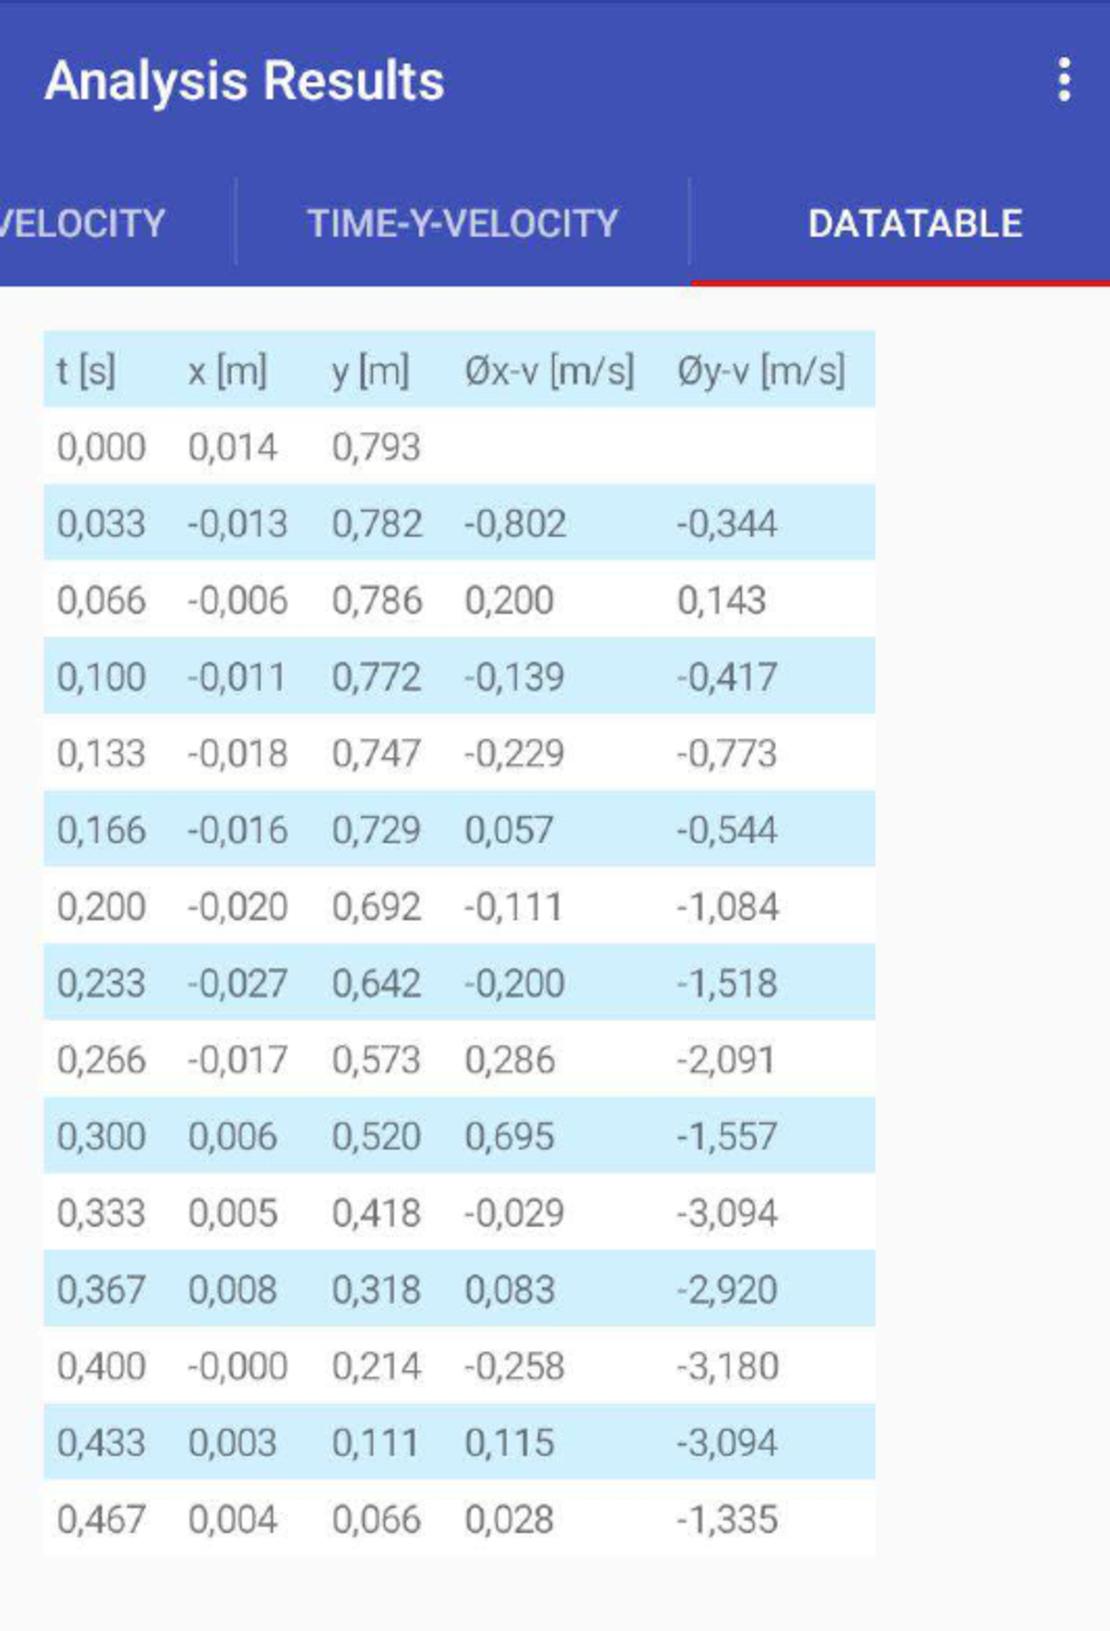
\includegraphics[width=8cm]{Figuras_exp3/imagenapendicec5.pdf}
\caption{\label{apendice5c} Tabela de dados gerada dentro do aplicativo VidAnalysis.}

\end{figure}
\chapter{Apêndice: $(E_f-E_i)/E_i$ a partir de traços e um ângulo}
\label{deltaE}


\vspace{-0.5cm}

Usando as equações para conservação de momento linear e balanço de energia, a variação percentual de energia cinética na colisão com massas iguais pode ser obtida a partir dos comprimentos e ângulos representados na Figura \ref{figcolisaomoedas3}. Chamando a velocidade da moeda A logo antes da colisão de $v_0$, e as velocidades das moedas A e B logo depois da colisão de $v_1$ e $v_2$, respectivamente, temos
\begin{equation}
    m_1 v_0 = m_1 v_1 \cos(\theta) + m_2 v_2 \cos(\phi),
\end{equation}
\begin{equation}
    0 = m_1 v_1 \sin(\theta) - m_2 v_2 \sin(\phi),
\end{equation}
\begin{equation}
    E_f - E_i = \frac{1}{2} m_1 v_1^2 +  \frac{1}{2} m_2 v_2^2 -  \frac{1}{2} m_1 v_0^2.
\end{equation}
Somando os quadrados das equações para conservação de momento linear em $x$ e em $y$
\begin{equation}
    m_1^2 v_0^2 = m_1^2 v_1^2  + m_2^2 v_2^2 + 2 m_1 m_2 v_1 v_2 \cos(\theta+\phi).
\end{equation}
Logo,
\begin{equation}
    E_f - E_i =   \frac{1}{2} m_2 \left(1-\frac{m_2}{m_1}\right) v_2^2  -  m_2 v_1 v_2 \cos(\theta+\phi),
\end{equation}

\begin{equation}
   \frac{ E_f - E_i}{E_i} =\frac{-1}{1-\frac{E_f}{E_i-E_f}}
   =\frac{-1}{1-
   \displaystyle {\frac{     \sqrt{\frac{m_1}{m_2}}\frac{v_1}{v_2} + \sqrt{\frac{m_2}{m_1}}\frac{v_2}{v_1}    }
   {    \left(1-\frac{m_2}{m_1}\right) \sqrt{\frac{m_2}{m_1}}\frac{v_2}{v_1} -2 \cos(\theta+\phi)}}  
   }.
\end{equation}
Se as moedas são iguais, as massas são iguais e também as forças de atrito entre cada moeda e a superfície. Neste caso, usando o teorema trabalho-energia cinética (aqui, $mv^2/2=F_{at} L$):
\begin{equation}
\frac{E_f - E_i}{E_i} = \frac{-1}{1+\displaystyle {\frac{\sqrt{\frac{L_A}{L_B}}+\sqrt{\frac{L_B}{L_A}}}{2~ \cos(\theta+\phi)}}}.
\label{eqEa}
\end{equation}
A Equação~\ref{eqEa} mostra que, para moedas iguais, a variação percentual de energia cinética na colisão pode ser obtida medindo apenas comprimentos e um ângulo entre trajetórias das duas, sem nem mesmo uma calibração para os comprimentos dos traços. Os dois parâmetros relevantes são (i) a razão entre entre os comprimentos dos traços depois da colisão, $L_A/L_B$, e (ii) a soma dos ângulos $\theta$ e $\phi$.  


%%%\chapter{Paquímetro}\label{paquimetro}

\vspace{-0.5cm}


O paquímetro é um instrumento utilizado para medir dimensões de objetos relativamente pequenos, desde uns poucos centímetros até frações de milímetros, com uma precisão da ordem do centésimo de milímetro. Este instrumento é delicado e deve ser manipulado com cuidado e precaução. 

Ele é formado por uma régua com um esquadro num extremo, sobre a qual se desliza o outro esquadro destinado a indicar o valor medido sobre a escala.  Sobre o esquadro móvel encontra-se o nônio que possui uma segunda escala dedicada a marcar as subdivisões do milímetro. Na Figura~\ref{fig:p1} podemos ver um desenho de um paquímetro típico.

\begin{figure}[h]
\begin{center}
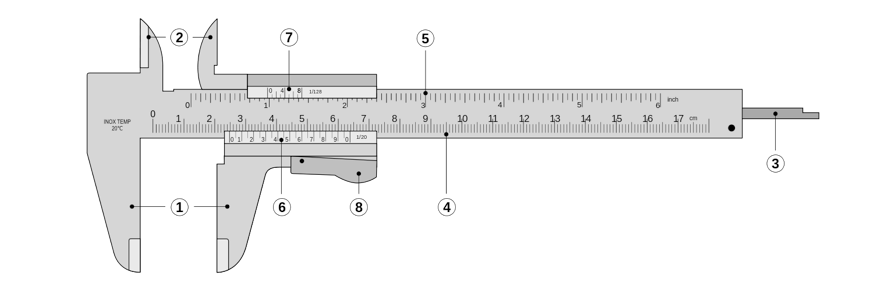
\includegraphics[width=14cm]{fig/Paquimetro1}
\caption{\label{fig:p1} Paquímetro formado por: \textcircled{1} Encostos para medidas externas; \textcircled{2} Orelhas para medidas internas; \textcircled{3} Haste de profundidade; \textcircled{4} Escala principal inferior (graduada em centímetros e milímetros); \textcircled{5} Escala principal superior (graduada em polegadas e frações de polegadas); \textcircled{6} Nônio ou vernier para leitura das frações de milímetros em que esteja dividido; \textcircled{7} Nônio ou vernier para leitura das frações de polegada em que esteja dividido; \textcircled{8} Propulsor e trava.}
\vspace{-0.5cm}
\end{center}
\end{figure}

Para utilizar o paquímetro, primeiramente se separam os encostos para que o objeto a ser medido possa ser colocado entre eles, logo se fecham estes encostos de forma que o objeto fique preso ao mesmo e se bloqueia o movimento do esquadro móvel para poder realizar a leitura do valor medido. Usaremos o exemplo mostrado na Figura~\ref{fig:p2} para facilitar a explicação de como fazer a leitura. 

\begin{figure}[h]
\begin{center}
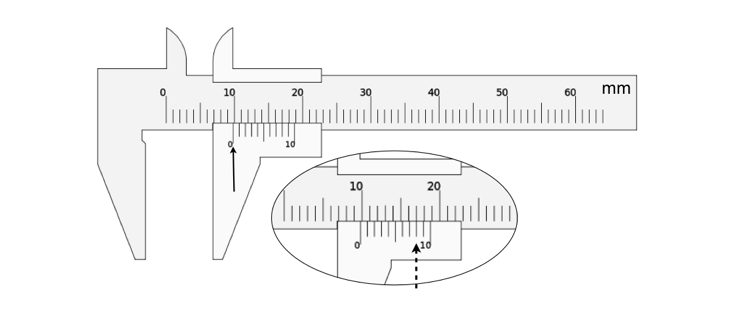
\includegraphics[width=14cm]{fig/Paquimetro2}
\caption{\label{fig:p2} Exemplo de uma medição realizada com paquímetro graduado em mm e com um nônio com 10 divisões. Valor medido (0,98 $\pm$ 0,01) cm. Ver texto.}
\vspace{-0.5cm}
\end{center}
\end{figure}

O primeiro passo é fazer a leitura sobre a escala principal (Figura~\ref{fig:p1}) e para isso observamos a posição do zero do nônio, que no exemplo está levemente deslocada à direita dos 9 mm (seta cheia na figura~\ref{fig:p2}). Desta forma temos a primeira parte da medida, sendo 0,9 cm. Vemos que as seguintes marcas do nônio também estão levemente deslocadas à direita e que esta diferença vai se reduzindo paulatinamente. Verificamos que a oitava marcação sobre o nônio coincide com a marcação com a régua principal (seta tracejada na Figura~\ref{fig:p2}) e logo as marcas do nônio vão ficando progressivamente à esquerda das marcas da régua fixa. Portanto a segunda parte da leitura nos diz que o valor medido é de 0,98 cm com uma incerteza de 0,01 cm.  Para a determinação da incerteza, considerada aqui como a mínima divisão do instrumento, temos que determinar o número de subdivisões do milímetro dado pelo nônio.  No caso do exemplo, temos 10 subdivisões, sendo a incerteza 1 mm dividido 10, ou seja 0,1 mm.  Finalmente o resultado da medição é: (0,98 $\pm$ 0,01) cm.

\underline {Importante:} Lembrar de verificar que o paquímetro esteja corretamente calibrado, ou seja que quando não haja abertura dos dois encostos, o zero da escala principal e do nônio sejam coincidentes.  

Mais informações sobre o uso do paquímetro podem ser encontradas na página  \url{http://www.stefanelli.eng.br/webpage/metrologia/p-nonio-milimetro-05.html}. Removido da Apostila (não usar no PLE)
%%%\chapter{Trilho de Ar}\label{trilho}
\vspace{-0.3cm}
O trilho de ar é um sistema que permite estudar movimentos unidimensionais reduzindo drasticamente as forças de atrito habitualmente presentes. Ele é composto de chapas metálicas de perfil reto, com pequenos orifícios regularmente espaçados nas faces  laterais.  

Injeta-se ar comprimido dentro do trilho que sai através dos orifícios gerando desta forma um colchão de ar entre o trilho e o carrinho de cerca de 0,5 mm de espessura. Este colchão de ar faz com que o carrinho "flutue", provocando assim uma grande redução do atrito.  O atrito residual é devido principalmente à fricção com o ar. Nas extremidades do trilho sempre deve-se colocar os pára-choques formado por um suporte com elásticos. 

O sistema trilho de ar e carrinho devem ser cuidadosamente tratados para evitar que eles se sofram deformações ou marcas que comprometam a redução do atrito.  Para isto devemos evitar choques mecânicos fortes, tanto ente o carrinho e o trilho como entre dois carrinhos. Evitar quedas dos carrinhos, mesmo que sejam de uns poucos centímetros, manuseando-os com segurança e muito cuidado. Em continuação enumeramos alguns cuidados extras na hora de utilizar o sistema trilho-carrinho, a saber:
\vspace{-0.3cm}
\begin{iten}

\item Nunca movimente os carrinhos sobre o trilho quando não houver ar saindo pelos orifícios do trilho ou se o ar que sai é muito fraco (neste caso deve se aumentar a potência do ar comprimido), pois serão produzidos arranhões.

\item Quando se colocar massas em cima dos carros, é fundamental que estas sejam distribuídas simetricamente para evitar desbalanceamentos do carrinho quando flutua podendo encostar certas partes dele no trilho.  Desta forma não só poderão ser produzidos arranhões no trilho senão como a hipóteses de atrito desprezível não será verificada. 

\item O trilho é apoiado sobre pequenas hastes numa base em perfil de alumínio. Estas hastes têm como função permitir o nivelamento do trilho. Com o tempo e o uso constante, o trilho de ar tende a se deformar criando "barrigas".  A consequência principal destas barrigas é os carrinhos passam a ter um movimento irregular. O nivelamento do trilho é uma operação trabalhosa e delicada, por isso deve-se estar seguro da necessidade de nivelamento antes de começar a mexer.

\end{iten}  Removido da Apostila (não usar no PLE)
%%%\chapter{Sistema de Video}\label{image}

\vspace{-0.5cm}

\section*{Configuração Câmera}

Para a realização dos filmes os passos a seguir são:

\begin{enumerate}
\item Ligue a câmera e verifique que o cartão de memória esteja vazio. %Para isto tem que ir ao menu e escolher com o cursor a terceira opção como é mostrado na Figura~\ref{fig:camera}-A. Uma vez no menu com o cursor da esquerda escolha a opção ``Apagar", dê ``OK" quantas vezes seja necessário para apagar as fotos e filmes do cartão de memória.

\item Configure a câmera para a realização do filme. 
\begin{itemize}
\item Para a câmera Olympus: %Entre no menu e escolha a segunda opção como indicado na Figura~\ref{fig:camera}-B.  A configuração escolhida deve ser: 
\begin{enumerate}
\item {\bf Tamanho De Imag} VGA
\item {\bf Imagens Por Seg.} 15 ou 30 fas (fotos por segundo) 
\item {\bf Microfone} Desl.  (desligado)
\item {\bf Modo AF}: configure a câmera para que sempre faça foco no objeto de interesse, mesmo quando ele esteja em movimento. Novamente, entre no menu e escolha a primeira opção como indicado na Figura~\ref{fig:camera}-C. No menu da esquerda escolha a terceira opção ``Modo AF" e logo ``Rastreia AF". Dê ``OK"  e pressione o botão do menu para sair do mesmo.
\end{enumerate}

\item Para a câmera Nikon Coolpix s3600, aperte o botão ``Menu", selecione o ícone de câmera de vídeo conforme a Figura~\ref{fig:nikon} e selecione:
\begin{enumerate}
\item {\bf Opções de vídeo}: 480/30p
\item {\bf Modo foco automático:} AF-F AF constante
\item {\bf VR do vídeo}: desligado
\end{enumerate}
\item Para a câmera Sony Cyber-shot, aperte o botão ``Menu" e busque as opções a seguir, conforme a Figura~\ref{fig:sony}: 
\begin{enumerate}
\item {\bf Tamanho Filme:} VGA
\item {\bf ACT:} STD movimentação moderada (nem todas as câmeras tem essa opção no menu à esquerda, com um ícone de mão)
\end{enumerate}
\end{itemize} 
\end{enumerate}

Desta forma sua câmera está configurada e você pode começar a fazer sua aquisição de dados. 
\begin{figure}[t!]
\begin{center}
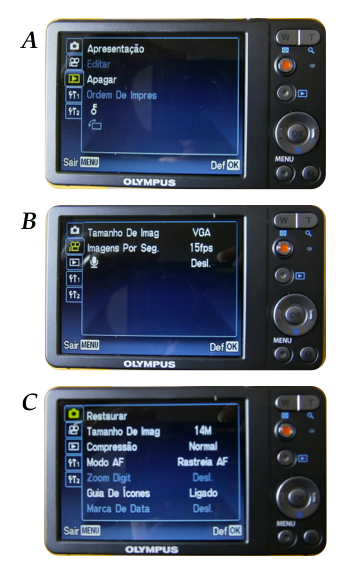
\includegraphics[width=9cm]{fig/CameraOlympus.png}
\caption{\label{fig:camera} Configuração da câmera Olympus.}
\vspace{-0.5cm}
\end{center}
\end{figure}

\begin{figure}[h!]
\begin{center}
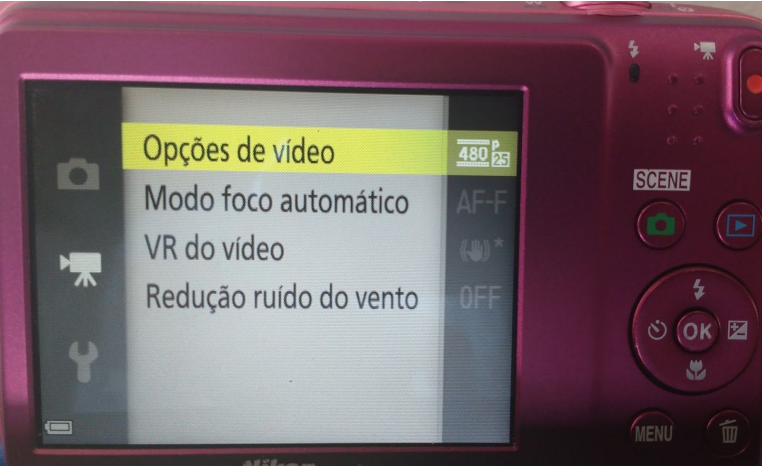
\includegraphics[width=9cm]{fig/cameraNikon.png}
\caption{\label{fig:nikon} Configuração da câmera Nikon.}
\vspace{-0.5cm}
\end{center}
\end{figure}

\begin{figure}[h!]
\begin{center}
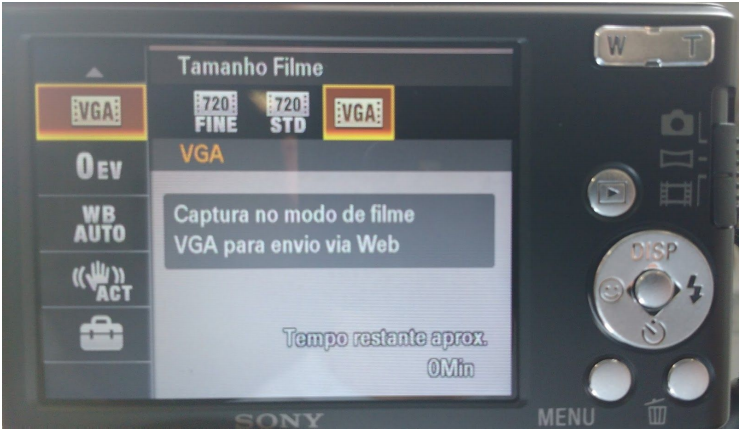
\includegraphics[width=9cm]{fig/cameraSony.png}
\caption{\label{fig:sony} Configuração da câmera Sony.}
\vspace{-0.5cm}
\end{center}
\end{figure}
\newpage
\section*{Leitura manual da posição do carrinho}
\begin{enumerate}

\item Uma vez registrado o movimento do carrinho com a câmera proceda a baixar o filme que você fez numa pasta no desktop do seu computador chamada MRU. Para algumas câmeras, o video é salvo no formato MP4 e precisa ser convertido em AVI para análise no programa ImageJ. Um tutorial para conversão dos videos encontra-se nas bancadas, próximo ao computador.
\item Abra o programa ImageJ.
\item No ImageJ abra o filme que você fez em formato AVI. Aparecerá uma tela com algumas indicações como se mostra na Figura~\ref{fig:frame}, “First Frame 1”, “Last Frame 135”, que podem em princípio ser alteradas pelo usuário. Essas informações correspondem ao número de imagens contidas no filme e permitem que escolhamos apenas algumas delas para serem exibidas. Mantenha como está e tecle “Ok”.
\begin{figure}[t!]
\begin{center}
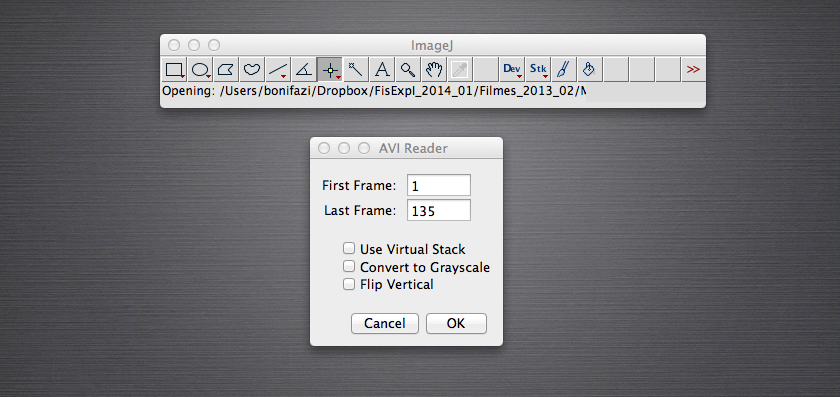
\includegraphics[width=11cm]{fig/frame}
\caption{\label{fig:frame} ImageJ: tela de inicio para carregar o filme.}
%\vspace{-0.5cm}
%\end{center}
%\end{figure}
%\begin{figure}[h]
%\begin{center}
\vspace{0.3cm}
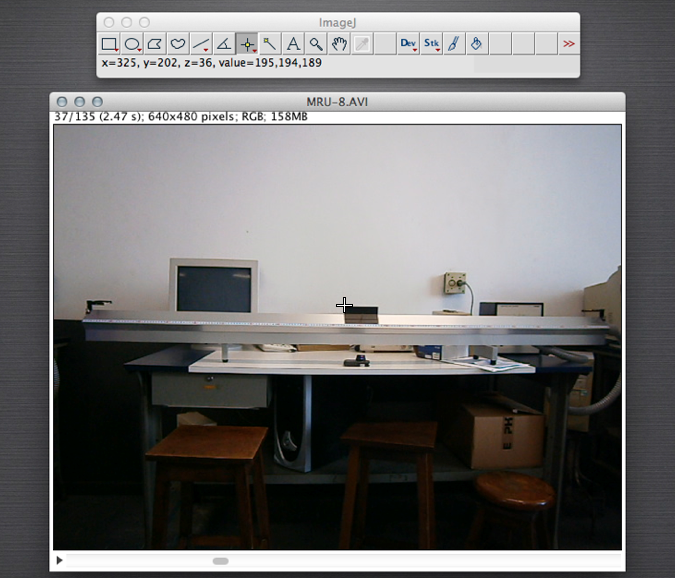
\includegraphics[width=11cm]{fig/cursor}
\caption{\label{fig:exMovie} ImageJ: posição do cursor sobre a imagem.}
\vspace{-0.6cm}
\end{center}
\end{figure}

\item Após o filme aberto você pode escolher a ferramenta de “zoom” que fica na barra de ferramentas do programa para ver melhor as imagens. A resolução das imagens não é muito boa, mas não precisamos mais do que isso para fazer a análise do experimento.
\item Experimente passar o cursor do mouse sobre a imagem. Você verá que embaixo da barra de ferramentas do ImageJ aparecerão alguns números, por exemplo, na Figura~\ref{fig:exMovie}: x=325, y=202, z=36, value = 195. As letras “x” e “y” correspondem à posição do cursor em “pixels” no sistema de referência mostrado na Figura~\ref{fig:exMovie}. A letra “z” corresponde à ordem em que imagem foi capturada em relação ao início do filme. Finalmente, “value” corresponde aos níveis de vermelho, verde e azul da imagem, nesta ordem. Para as análises que faremos, só utilizaremos a posição “x e y” do cursor.
\item Observe agora no canto superior esquerdo das imagens do filme (Figura~\ref{fig:exMovie}). Aparecem números semelhantes a “37/135 (2.47s); 640x480 pixels; RGB; 158 MB”. O primeiro deles significa que está sendo exibida a imagem 37 de um total de 135. O instante de tempo no qual essa imagem foi capturada em relação ao início do filme é indicado pelo número entre parênteses “2.47s” que é dado por $1/15 \times 37$~s (onde 1/15 corresponde a 15 fotos ou {\it frames}  por segundo), “640 X 480 pixels” corresponde às dimensões da imagem em número de “pixels”, “RGB” corresponde à qualidade da imagem, e “158 MB” corresponde ao espaço de memória do computador que foi utilizado para guardar o filme. Para nossas análises o número importante dentre esses é o que corresponde ao número de imagem e ao instante de tempo em que a imagem foi capturada. \underline{Observação}: estes números serão diferentes para cada filme.
\end{enumerate}


\section*{Rotação do Filme}

Para realizar a análise dos dados, é necessário que a medida do deslocamento do carrinho seja apenas em uma dimensão, por exemplo, na horizontal.  Se o eixo horizontal da câmera não está bem alinhado com o trilho, precisamos realizar uma rotação do filme antes de proceder à leitura da posição do carrinho. Portanto, o primeiro passo é a determinação do ângulo de rotação.  A mesma pode ser realizada de duas formas diferentes:

\vspace{-0.7cm}
\subsection*{\underline{Forma manual}}
\vspace{-0.2cm}
\begin{enumerate}
\item Determine com os cursores as coordenadas ``x e y" das extremidades do trilho, tendo desta forma $(x_1,y_1) e (x_2, y_2)$ como se mostra na figura~\ref{fig:coord}.
\item Utilizando trigonometria, e utilizando uma calculadora, determine o ângulo de inclinação como o $\arctan{(y_2-y_1)/(x_2-x_1)}$. \underline{Observação:} o ângulo tem que ser determinado em graus.
\end{enumerate}

\vspace{-0.9cm}
\subsection*{\underline{Forma automática}}
\vspace{-0.2cm}
\begin{enumerate}
\item Escolha o botão de “\^Angulo” (círculo na Figura~\ref{fig:angulo}-A), que fica na barra de ferramentas do programa ImageJ para poder marcar o ângulo que quer ser determinado. 
\item Movimente o cursor para marcar os três pontos que vão determinar o ângulo que o trilho forma com a horizontal (linhas cheias sobre o filme na Figura~\ref{fig:angulo}-B). Faça click cada vez que esteja na posição desejada.
\item Escolha a opção "Analyze" do menu principal e "Measure" do sub-menu.
\item O resultado será mostrado em uma outra janela (Figura~\ref{fig:angRes}), entre os quais estará o valor do ângulo desejado em graus.

\begin{figure}[t!]
\begin{center}
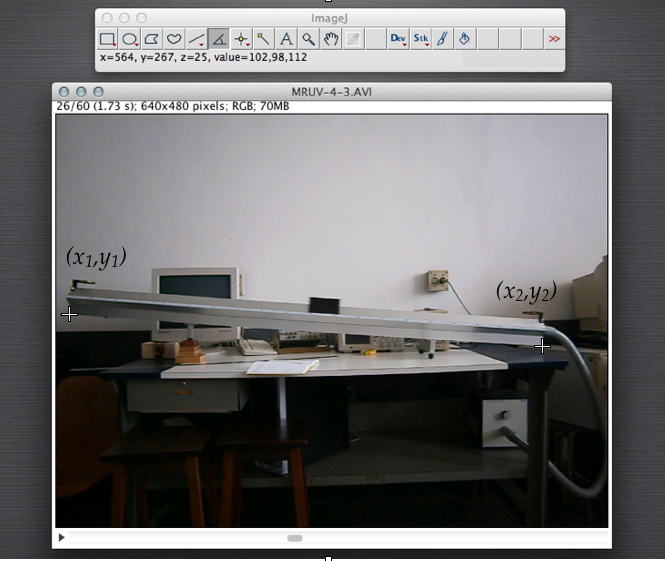
\includegraphics[width=9cm]{fig/coordman}
\caption{\label{fig:coord} ImageJ: determinação das coordenadas $(x_1,y_1) e (x_2, y_2)$, ver texto.}
\vspace{0.5cm}
%\end{center}
%\end{figure}
%\begin{figure}[h]
%\begin{center}
%\vspace{-0.3cm}
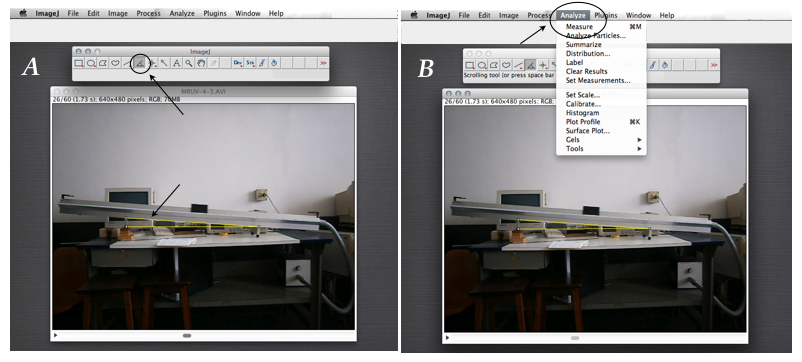
\includegraphics[width=16cm]{fig/AnguloAuto}
\caption{\label{fig:angulo} ImageJ: determinação do ângulo de inclinação do trilho, ver texto.}
\vspace{-0.5cm}
\end{center}
\end{figure}

Uma vez determinado o ângulo, devemos proceder a realizar a rotação do Filme. Para isto, deve seguir os seguintes passos: 
\begin{enumerate}
\item Escolha a opção ``Imagem" do menu principal, logo ``Transform" e finalmente ``Rotate", como mostrado na Figura~\ref{fig:rotate}-A.
\item Uma nova janela será aberta onde deve-ser informado o valor do ângulo de rotação, no nosso exemplo, o mesmo é de 4,101 graus (Figura~\ref{fig:angRes}). Este ângulo deve ser informado com o sinal negativo ($-$) se queremos realizar uma rotação no sentido anti-horário ou com sinal positivo ($+$) se a rotação é no sentido horário.
\item {\bf Como a rotação é uma ação definitiva} e não pode ser refeita, utilizar sempre o ``Preview" para poder ter certeza de que se está realizando a rotação desejada (ver Figura~\ref{fig:rotate}-B) antes de dar o ``OK" final.
\end{enumerate}

\begin{figure}[h!]
\begin{center}
\vspace{0.3cm}
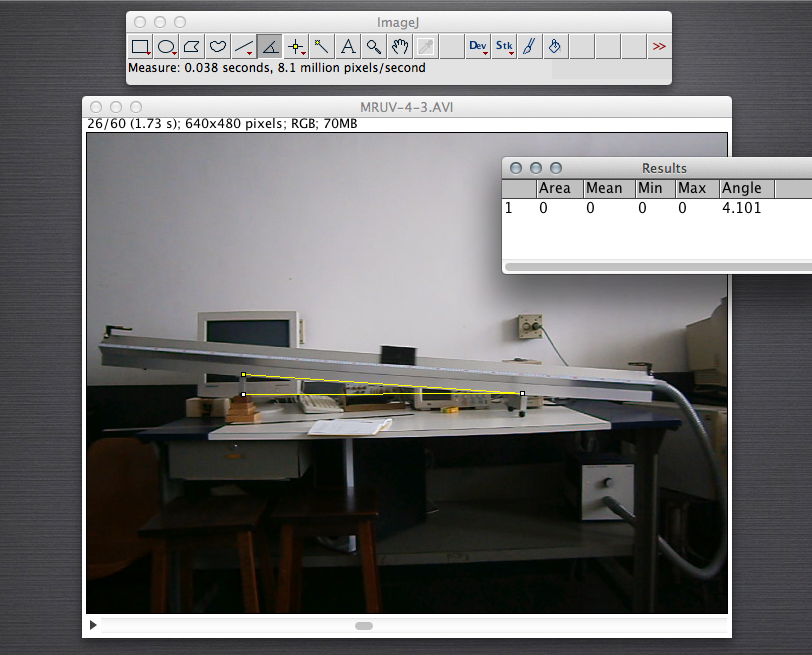
\includegraphics[width=10cm]{fig/AnguloResultado}
\caption{\label{fig:angRes} ImageJ: valor do ângulo de inclinação do trilho}
\vspace{0.5cm}
%\end{center}
%\end{figure}
%\begin{figure}[h]
%\begin{center}
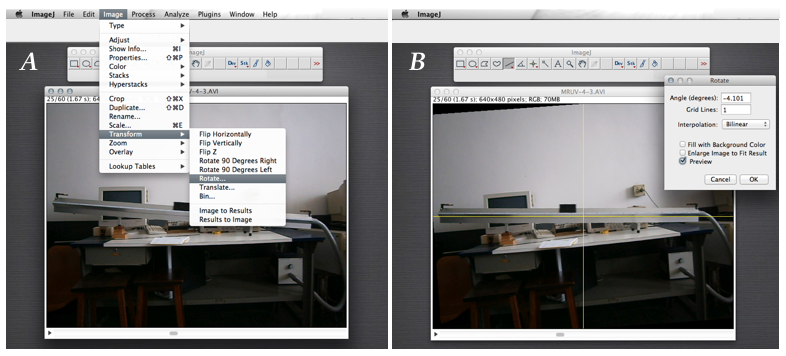
\includegraphics[width=16cm]{fig/Rotate}
\caption{\label{fig:rotate} ImageJ: rotação do filme por um determinado ângulo, ver texto}
\vspace{-0.5cm}
\end{center}
\end{figure}
\end{enumerate}
  Removido da Apostila (não usar no PLE)
%\chapter{Programa QtiPlot}\label{QtiPlot}

\vspace{-0.7cm}

Ao longo do curso vamos realizar gráficos e ajustes lineares (ajustes por uma reta), para isto vamos aprender a utilizar um programa chamado de QtiPlot.  Este programa pode ser baixado gratuitamente da internet, ou da página pessoal do Prof. Angelo Gomes em: 
\url{http://www.if.ufrj.br/~amgomes/qtiplotinfo.html}. 

Para descompactar o mesmo você deverá fornecer uma senha, a mesma é: fisexp2-2009

O Prof. Angelo Gomes preparou um tutorial que ajuda a aprender a utilizar o QtiPlot. Para acessar ao mesmo, basta com ir para \\
\url{http://www.if.ufrj.br/~amgomes/tutorialqtiplot-pag1.html}

Qualquer dúvida ou problema, entrar em contato com seu professor e/ou monitor.
 Removido da Apostila (não usar no PLE)

\end{document}

%%%%%%%%%%%%%%%%%%%%%%%%%%%%%%
